% Generated by Sphinx.
\def\sphinxdocclass{report}
\documentclass[letterpaper,10pt,english]{sphinxmanual}
\usepackage[utf8]{inputenc}
\DeclareUnicodeCharacter{00A0}{\nobreakspace}
\usepackage[T1]{fontenc}
\usepackage{babel}
\usepackage{times}
\usepackage[Bjarne]{fncychap}
\usepackage{longtable}
\usepackage{sphinx}


\title{Gemini AstroData Type Reference}
\date{March 09, 2012}
\release{1.00}
\author{Craig Allen}
\newcommand{\sphinxlogo}{}
\renewcommand{\releasename}{Release}
\makeindex

\makeatletter
\def\PYG@reset{\let\PYG@it=\relax \let\PYG@bf=\relax%
    \let\PYG@ul=\relax \let\PYG@tc=\relax%
    \let\PYG@bc=\relax \let\PYG@ff=\relax}
\def\PYG@tok#1{\csname PYG@tok@#1\endcsname}
\def\PYG@toks#1+{\ifx\relax#1\empty\else%
    \PYG@tok{#1}\expandafter\PYG@toks\fi}
\def\PYG@do#1{\PYG@bc{\PYG@tc{\PYG@ul{%
    \PYG@it{\PYG@bf{\PYG@ff{#1}}}}}}}
\def\PYG#1#2{\PYG@reset\PYG@toks#1+\relax+\PYG@do{#2}}

\def\PYG@tok@gd{\def\PYG@tc##1{\textcolor[rgb]{0.63,0.00,0.00}{##1}}}
\def\PYG@tok@gu{\let\PYG@bf=\textbf\def\PYG@tc##1{\textcolor[rgb]{0.50,0.00,0.50}{##1}}}
\def\PYG@tok@gt{\def\PYG@tc##1{\textcolor[rgb]{0.00,0.25,0.82}{##1}}}
\def\PYG@tok@gs{\let\PYG@bf=\textbf}
\def\PYG@tok@gr{\def\PYG@tc##1{\textcolor[rgb]{1.00,0.00,0.00}{##1}}}
\def\PYG@tok@cm{\let\PYG@it=\textit\def\PYG@tc##1{\textcolor[rgb]{0.25,0.50,0.56}{##1}}}
\def\PYG@tok@vg{\def\PYG@tc##1{\textcolor[rgb]{0.73,0.38,0.84}{##1}}}
\def\PYG@tok@m{\def\PYG@tc##1{\textcolor[rgb]{0.13,0.50,0.31}{##1}}}
\def\PYG@tok@mh{\def\PYG@tc##1{\textcolor[rgb]{0.13,0.50,0.31}{##1}}}
\def\PYG@tok@cs{\def\PYG@tc##1{\textcolor[rgb]{0.25,0.50,0.56}{##1}}\def\PYG@bc##1{\colorbox[rgb]{1.00,0.94,0.94}{##1}}}
\def\PYG@tok@ge{\let\PYG@it=\textit}
\def\PYG@tok@vc{\def\PYG@tc##1{\textcolor[rgb]{0.73,0.38,0.84}{##1}}}
\def\PYG@tok@il{\def\PYG@tc##1{\textcolor[rgb]{0.13,0.50,0.31}{##1}}}
\def\PYG@tok@go{\def\PYG@tc##1{\textcolor[rgb]{0.19,0.19,0.19}{##1}}}
\def\PYG@tok@cp{\def\PYG@tc##1{\textcolor[rgb]{0.00,0.44,0.13}{##1}}}
\def\PYG@tok@gi{\def\PYG@tc##1{\textcolor[rgb]{0.00,0.63,0.00}{##1}}}
\def\PYG@tok@gh{\let\PYG@bf=\textbf\def\PYG@tc##1{\textcolor[rgb]{0.00,0.00,0.50}{##1}}}
\def\PYG@tok@ni{\let\PYG@bf=\textbf\def\PYG@tc##1{\textcolor[rgb]{0.84,0.33,0.22}{##1}}}
\def\PYG@tok@nl{\let\PYG@bf=\textbf\def\PYG@tc##1{\textcolor[rgb]{0.00,0.13,0.44}{##1}}}
\def\PYG@tok@nn{\let\PYG@bf=\textbf\def\PYG@tc##1{\textcolor[rgb]{0.05,0.52,0.71}{##1}}}
\def\PYG@tok@no{\def\PYG@tc##1{\textcolor[rgb]{0.38,0.68,0.84}{##1}}}
\def\PYG@tok@na{\def\PYG@tc##1{\textcolor[rgb]{0.25,0.44,0.63}{##1}}}
\def\PYG@tok@nb{\def\PYG@tc##1{\textcolor[rgb]{0.00,0.44,0.13}{##1}}}
\def\PYG@tok@nc{\let\PYG@bf=\textbf\def\PYG@tc##1{\textcolor[rgb]{0.05,0.52,0.71}{##1}}}
\def\PYG@tok@nd{\let\PYG@bf=\textbf\def\PYG@tc##1{\textcolor[rgb]{0.33,0.33,0.33}{##1}}}
\def\PYG@tok@ne{\def\PYG@tc##1{\textcolor[rgb]{0.00,0.44,0.13}{##1}}}
\def\PYG@tok@nf{\def\PYG@tc##1{\textcolor[rgb]{0.02,0.16,0.49}{##1}}}
\def\PYG@tok@si{\let\PYG@it=\textit\def\PYG@tc##1{\textcolor[rgb]{0.44,0.63,0.82}{##1}}}
\def\PYG@tok@s2{\def\PYG@tc##1{\textcolor[rgb]{0.25,0.44,0.63}{##1}}}
\def\PYG@tok@vi{\def\PYG@tc##1{\textcolor[rgb]{0.73,0.38,0.84}{##1}}}
\def\PYG@tok@nt{\let\PYG@bf=\textbf\def\PYG@tc##1{\textcolor[rgb]{0.02,0.16,0.45}{##1}}}
\def\PYG@tok@nv{\def\PYG@tc##1{\textcolor[rgb]{0.73,0.38,0.84}{##1}}}
\def\PYG@tok@s1{\def\PYG@tc##1{\textcolor[rgb]{0.25,0.44,0.63}{##1}}}
\def\PYG@tok@gp{\let\PYG@bf=\textbf\def\PYG@tc##1{\textcolor[rgb]{0.78,0.36,0.04}{##1}}}
\def\PYG@tok@sh{\def\PYG@tc##1{\textcolor[rgb]{0.25,0.44,0.63}{##1}}}
\def\PYG@tok@ow{\let\PYG@bf=\textbf\def\PYG@tc##1{\textcolor[rgb]{0.00,0.44,0.13}{##1}}}
\def\PYG@tok@sx{\def\PYG@tc##1{\textcolor[rgb]{0.78,0.36,0.04}{##1}}}
\def\PYG@tok@bp{\def\PYG@tc##1{\textcolor[rgb]{0.00,0.44,0.13}{##1}}}
\def\PYG@tok@c1{\let\PYG@it=\textit\def\PYG@tc##1{\textcolor[rgb]{0.25,0.50,0.56}{##1}}}
\def\PYG@tok@kc{\let\PYG@bf=\textbf\def\PYG@tc##1{\textcolor[rgb]{0.00,0.44,0.13}{##1}}}
\def\PYG@tok@c{\let\PYG@it=\textit\def\PYG@tc##1{\textcolor[rgb]{0.25,0.50,0.56}{##1}}}
\def\PYG@tok@mf{\def\PYG@tc##1{\textcolor[rgb]{0.13,0.50,0.31}{##1}}}
\def\PYG@tok@err{\def\PYG@bc##1{\fcolorbox[rgb]{1.00,0.00,0.00}{1,1,1}{##1}}}
\def\PYG@tok@kd{\let\PYG@bf=\textbf\def\PYG@tc##1{\textcolor[rgb]{0.00,0.44,0.13}{##1}}}
\def\PYG@tok@ss{\def\PYG@tc##1{\textcolor[rgb]{0.32,0.47,0.09}{##1}}}
\def\PYG@tok@sr{\def\PYG@tc##1{\textcolor[rgb]{0.14,0.33,0.53}{##1}}}
\def\PYG@tok@mo{\def\PYG@tc##1{\textcolor[rgb]{0.13,0.50,0.31}{##1}}}
\def\PYG@tok@mi{\def\PYG@tc##1{\textcolor[rgb]{0.13,0.50,0.31}{##1}}}
\def\PYG@tok@kn{\let\PYG@bf=\textbf\def\PYG@tc##1{\textcolor[rgb]{0.00,0.44,0.13}{##1}}}
\def\PYG@tok@o{\def\PYG@tc##1{\textcolor[rgb]{0.40,0.40,0.40}{##1}}}
\def\PYG@tok@kr{\let\PYG@bf=\textbf\def\PYG@tc##1{\textcolor[rgb]{0.00,0.44,0.13}{##1}}}
\def\PYG@tok@s{\def\PYG@tc##1{\textcolor[rgb]{0.25,0.44,0.63}{##1}}}
\def\PYG@tok@kp{\def\PYG@tc##1{\textcolor[rgb]{0.00,0.44,0.13}{##1}}}
\def\PYG@tok@w{\def\PYG@tc##1{\textcolor[rgb]{0.73,0.73,0.73}{##1}}}
\def\PYG@tok@kt{\def\PYG@tc##1{\textcolor[rgb]{0.56,0.13,0.00}{##1}}}
\def\PYG@tok@sc{\def\PYG@tc##1{\textcolor[rgb]{0.25,0.44,0.63}{##1}}}
\def\PYG@tok@sb{\def\PYG@tc##1{\textcolor[rgb]{0.25,0.44,0.63}{##1}}}
\def\PYG@tok@k{\let\PYG@bf=\textbf\def\PYG@tc##1{\textcolor[rgb]{0.00,0.44,0.13}{##1}}}
\def\PYG@tok@se{\let\PYG@bf=\textbf\def\PYG@tc##1{\textcolor[rgb]{0.25,0.44,0.63}{##1}}}
\def\PYG@tok@sd{\let\PYG@it=\textit\def\PYG@tc##1{\textcolor[rgb]{0.25,0.44,0.63}{##1}}}

\def\PYGZbs{\char`\\}
\def\PYGZus{\char`\_}
\def\PYGZob{\char`\{}
\def\PYGZcb{\char`\}}
\def\PYGZca{\char`\^}
\def\PYGZsh{\char`\#}
\def\PYGZpc{\char`\%}
\def\PYGZdl{\char`\$}
\def\PYGZti{\char`\~}
% for compatibility with earlier versions
\def\PYGZat{@}
\def\PYGZlb{[}
\def\PYGZrb{]}
\makeatother

\begin{document}

\maketitle
\setcounter{tocdepth}{6}
\tableofcontents
\phantomsection\label{chapter_Gemini_Types::doc}



\chapter{Introduction}
\label{gatref/GATREF-introduction:introduction}\label{gatref/GATREF-introduction:gemini-astrodata-types-reference}\label{gatref/GATREF-introduction::doc}

\section{Document Brief}
\label{gatref/gatrefdocbrief:document-brief}\label{gatref/gatrefdocbrief::doc}

\subsection{Revision History}
\label{gatref/gen.GATREF-RevisionHistory:revision-history}\label{gatref/gen.GATREF-RevisionHistory::doc}\begin{itemize}
\item {} 
v0.2.(20120310001559) - Revision incremented at 01:41, 5 May 2010
(UTC)

\end{itemize}


\subsection{Document Purpose}
\label{gatref/gen.GATREF-Purpose::doc}\label{gatref/gen.GATREF-Purpose:document-purpose}
This document is intended as an up to date reference manual for the
Gemini AstroData Type library defined within the ADCONFIG\_Gemini
configuration package. Where possible the document is created by
inspecting the configuration package itself, i.e. to create correct
graphs for type trees. This document records the current state of the
configuration. For more information on altering it or making your own
configuration, see the ``AstroData Package Manual'', available at \href{http://ophiuchus.hi.gemini.edu/ADDOCS/\_latex\_build/astrodatadocumentation.pdf}{http:
//ophiuchus.hi.gemini.edu/ADDOCS/\_latex\_build/astrodatadocumentation.p
df} \textbf{(internal to Gemini, external link not yet
available)}.


\subsection{Intended Audience}
\label{gatref/gen.GATREF-Audience::doc}\label{gatref/gen.GATREF-Audience:intended-audience}
This reference is intended for all users of the Gemini AstroData
Package, as well as developers maintaining or augmenting type
information.


\section{Overview}
\label{gatref/GATREF-overview:overview}\label{gatref/GATREF-overview::doc}
In order to configure astrodata with the Gemini data types and descriptors, the
astrodata package must be able to find the ADCONFIG package in which they are
defined. The ADCONFIG packages must be within a subdirectory called
``ADCONFIG\_\textless{}whatever\textgreater{}'', the Gemini package is ``ADCONFIG\_Gemini''. The astrodata
package will search the PYTHONPATH for these packages.  While they do contain
python code, they are not meant to be directly imported, and PYTHONPATH is used
to make installation simpler. One can also set ADCONFIGPATH.  Note: the PATH
environment variable point to the parent directory, which contains the
``{\color{red}\bfseries{}ADCONFIG\_}...'' subdirectory.


\chapter{Gemini Type Graphs}
\label{appendix_typegraphs:gemini-type-graphs}\label{appendix_typegraphs::doc}
Gemini dataset types, or ``AstroData Types'' include three distinct trees.
\begin{itemize}
\item {} 
The GEMINI tree which relates to instruments and instrument-modes.

\item {} 
The RAW tree which is single descendant, and represents processing status.
These types are presented mixed with the ``typological'' types through
the getTypes interface, but can also be retrieves through the getStatus call.

\item {} 
A generic type tree which relates to the GEMINI tree (i.e. IMAGE is any
of the specific INSTR\_IMAGE types.

\end{itemize}

The graphs below are derived from the ADCONFIG\_Gemini AstroData Configuration
Package as of March 09, 2012, and show descriptor and primitive set assignments when present.


\section{GENERIC}
\label{appendix_typegraphs:generic}
The GENERIC type tree relates to abstract data modes which may be used to apply recipes generic to these modes.  If generic primitives
can be written, these too can be shared, but it is also possible to assign the primitives at instrument-mode specific granularity as
well. That is, one can provide generic code at the levels where it makes sense, and type-specific code when that makes more sense or is
expedient.  We generally visualize an incremental development process where new instrument-modes are first supported  in type-specific code where
changes to the system are isolated and don't affect other processing. Subsequently this code can be integrated into, or merely replaced
by, more general algorithms that use other AstroData features to abstract away incidental differences between datasets from different
devices.
\begin{figure}[htbp]
\centering
\capstart

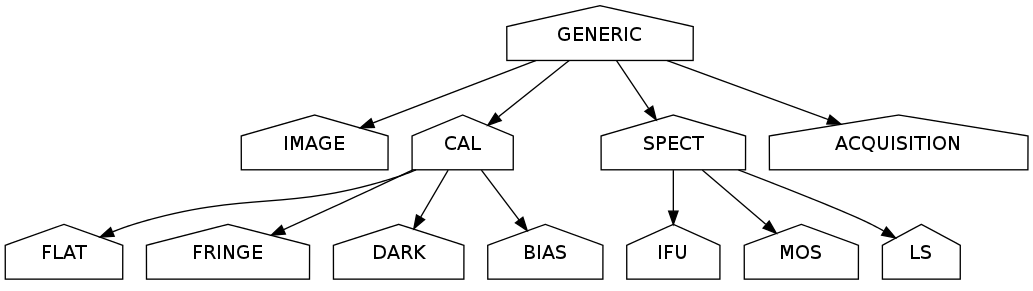
\includegraphics[width=0.900\linewidth]{GENERIC-tree-pd.png}
\caption{The Gemini GENERIC Type Tree}\end{figure}


\section{GEMINI}
\label{appendix_typegraphs:gemini}
The complete tree of instrument-mode related typological classifications all
descend from the GEMINI type, which means of course, the data was from a
GEMINI telescope. The figure is difficult to read as all types are present, and
will get more so as the instrument trees are filled out.  The instrument related
graphs are more informative, but this gives and idea of the overall taxology.
\begin{figure}[htbp]
\centering
\capstart

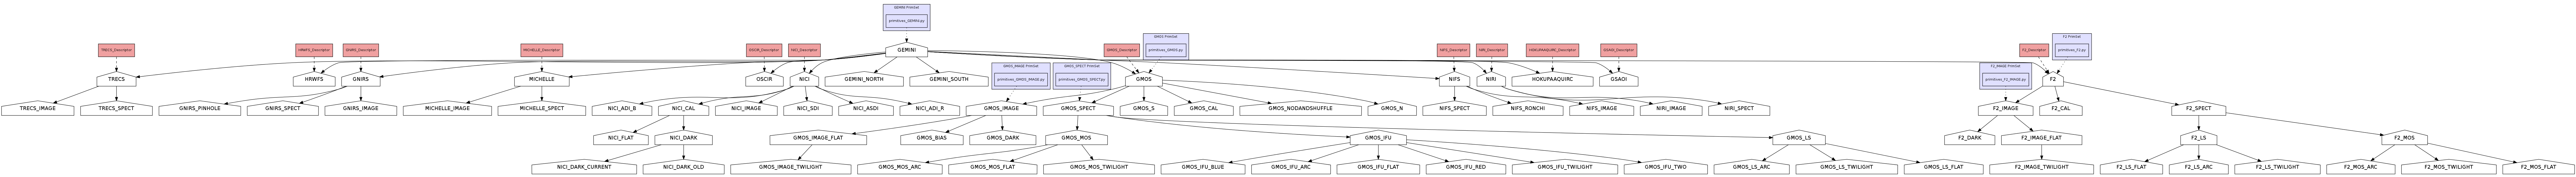
\includegraphics[width=1.000\linewidth]{GEMINI-tree-pd.png}
\caption{The Gemini GEMINI Type Tree}\end{figure}


\section{GMOS}
\label{appendix_typegraphs:gmos}
GMOS is an optical instrument with an imaging mode, an IFU, and a multi-object
spectrograph. We have a complete first revision of the GMOS tree.
\begin{figure}[htbp]
\centering
\capstart

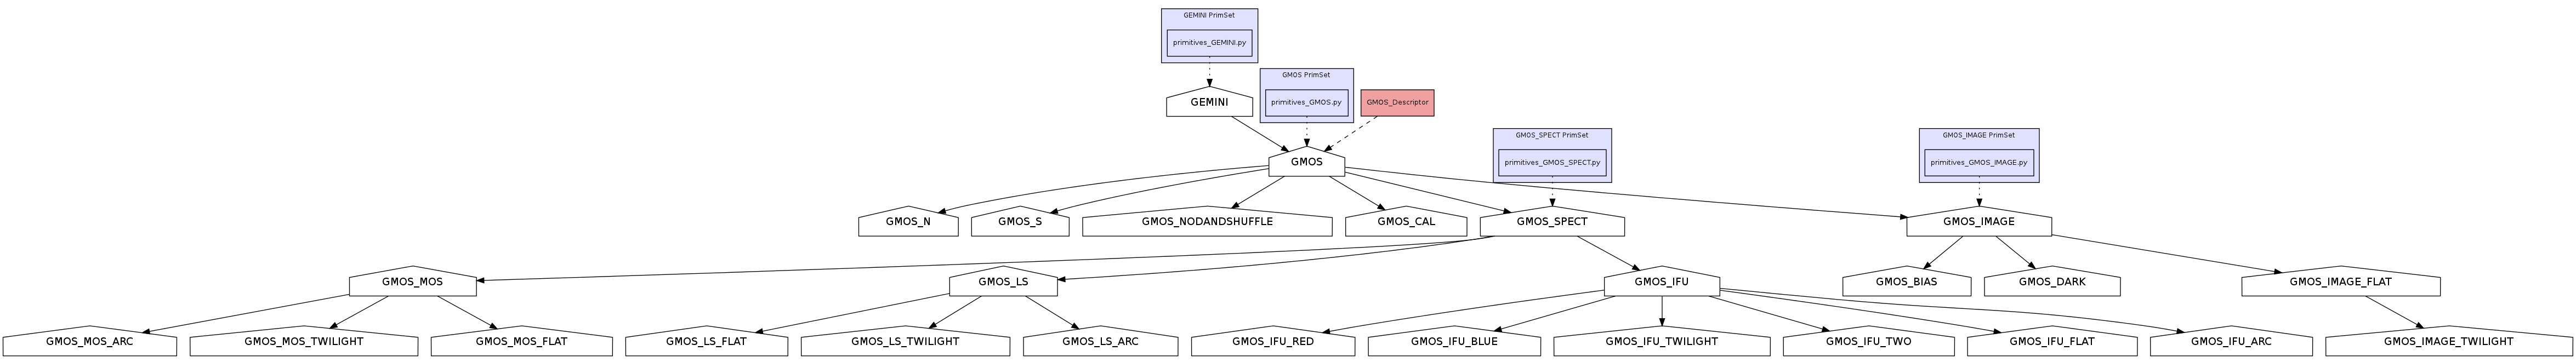
\includegraphics[width=0.900\linewidth]{GMOS-tree-pd.png}
\caption{The Gemini GMOS Type Tree}\end{figure}


\section{GNIRS}
\label{appendix_typegraphs:gnirs}
GNIRS is a near-infrared spectroscopy instrument currently under repair. The
tree is just a stub, which recognizes data from GNIRS.
\begin{figure}[htbp]
\centering
\capstart

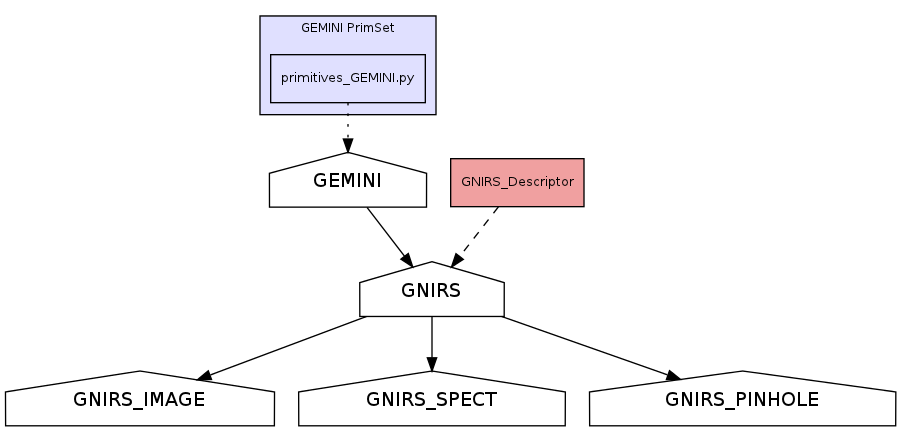
\includegraphics[width=0.200\linewidth]{GNIRS-tree-pd.png}
\caption{The Gemini GNIRS Type Tree}\end{figure}


\section{NICI}
\label{appendix_typegraphs:nici}
NICI is the Near-Infrared Coronagraphic Imager, used at Gemini South. We have a
preliminary (development) first revision of the NICI type tree.
\begin{figure}[htbp]
\centering
\capstart

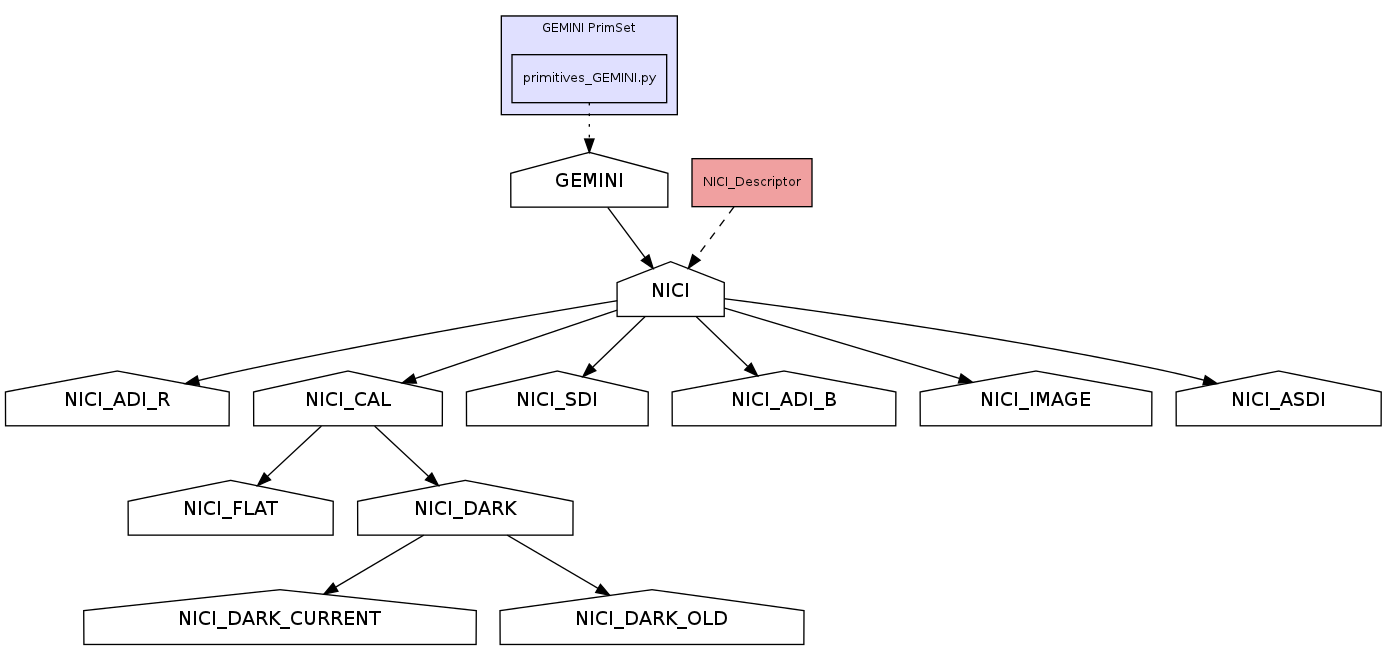
\includegraphics[width=0.750\linewidth]{NICI-tree-pd.png}
\caption{The Gemini NICI Type Tree}\end{figure}


\section{NIFS}
\label{appendix_typegraphs:nifs}
NIFS is a Near-Infrared Integral Field Spectrometer  uses at Gemini North.  We
have a minimal tree in place for NIFS, which recognizes IMAGE and SPECT types.
\begin{figure}[htbp]
\centering
\capstart

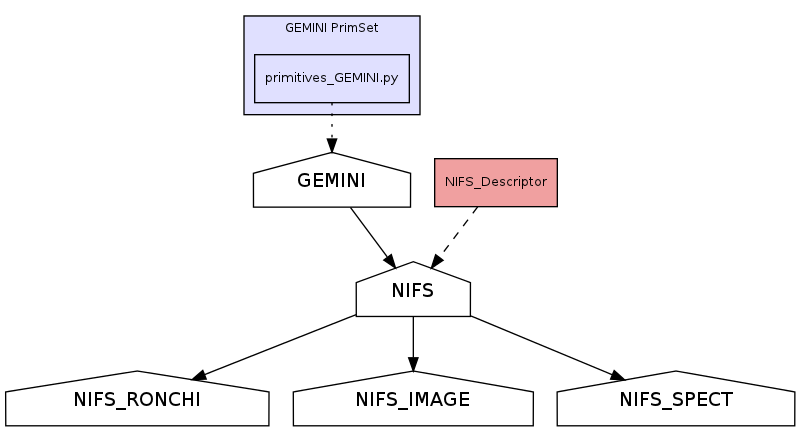
\includegraphics[width=0.300\linewidth]{NIFS-tree-pd.png}
\caption{The Gemini NIFS Type Tree}\end{figure}


\section{NIRI}
\label{appendix_typegraphs:niri}
NIRI is a Near-Infrared Imager in use at Gemini North. We have a minimal tree in
place for NIRI, which recognizes IMAGE and SPECT types.
\begin{figure}[htbp]
\centering
\capstart

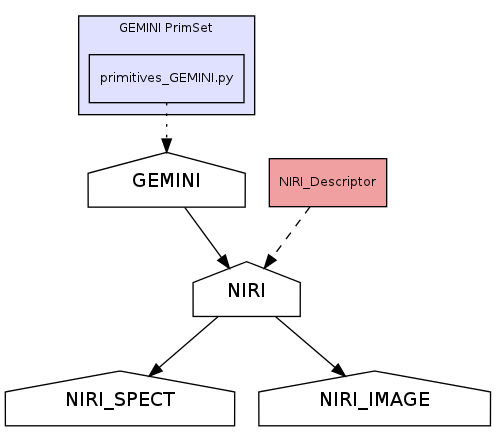
\includegraphics[width=0.300\linewidth]{NIRI-tree-pd.png}
\caption{The Gemini NIRI Type Tree}\end{figure}


\section{MICHELLE}
\label{appendix_typegraphs:michelle}
MICHELLE is a mid-infrared image and sepctrometer. We have a minimal tree in
place for MICHELLE, which recognizes IMAGE and SPECT types.
\begin{figure}[htbp]
\centering
\capstart

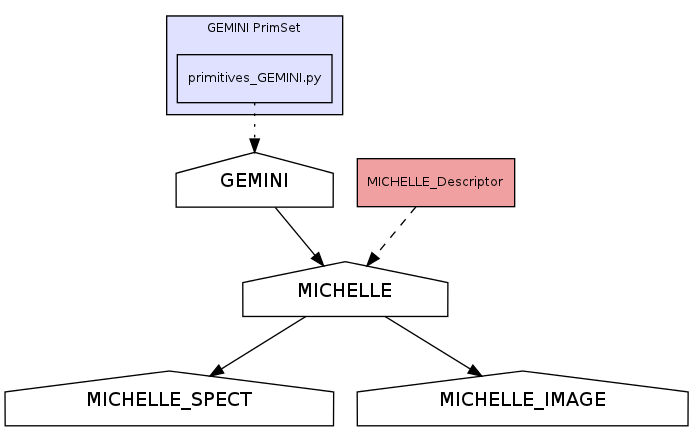
\includegraphics[width=0.300\linewidth]{MICHELLE-tree-pd.png}
\caption{The Gemini MICHELLE Type Tree}\end{figure}


\section{RAW}
\label{appendix_typegraphs:raw}
The RAW tree contains inherent sequencing, what are show as children are new
forms of the data... that is, some transformation(s) will make the data
recognized only as the child.  These types can be used to check the state of
processing, and can have entirely generic recipes associated, as may be needed
by some pipelines.
\begin{figure}[htbp]
\centering
\capstart

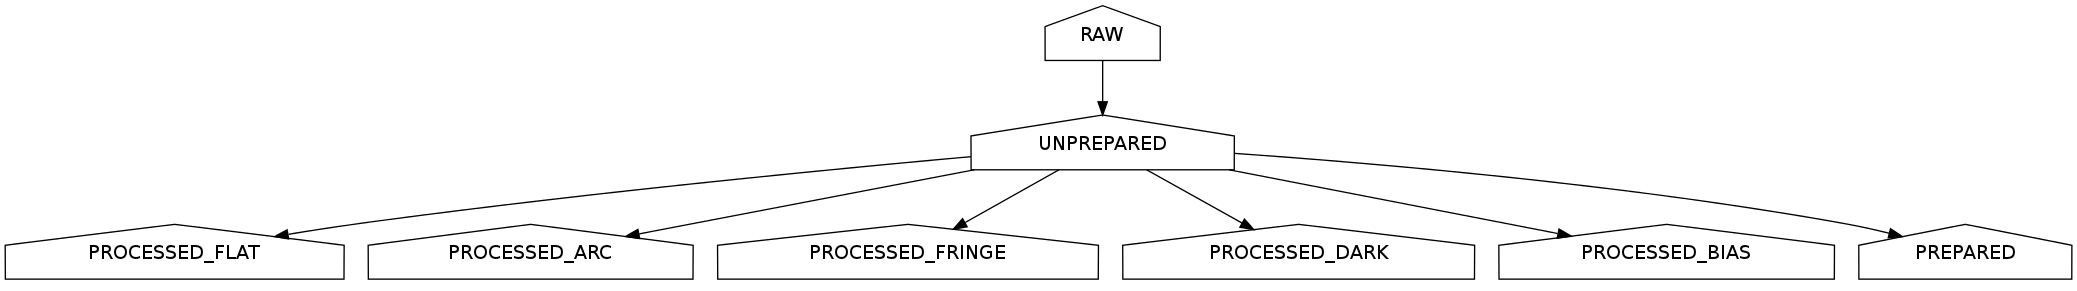
\includegraphics[width=0.600\linewidth]{RAW-tree-pd.png}
\caption{The Gemini RAW Type Tree}\end{figure}


\section{TRECS}
\label{appendix_typegraphs:trecs}
TRECS is a Thermal-Region Camera Spectograph, a mid-infrared imager and
long-slit spectrograph built  for Gemini South. We have a minimal tree in place
for TRECS, which recognizes IMAGE and SPECT.
\begin{figure}[htbp]
\centering
\capstart

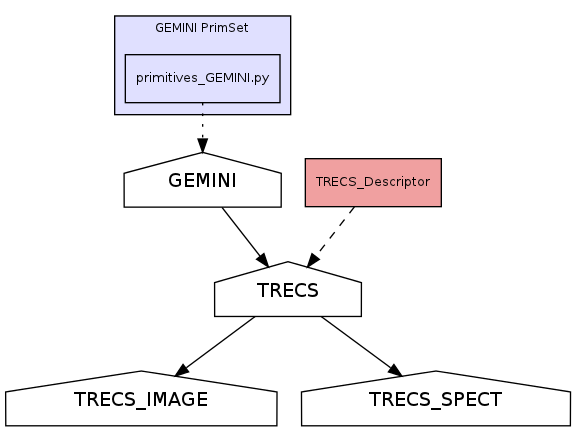
\includegraphics[width=0.300\linewidth]{TRECS-tree-pd.png}
\caption{The Gemini TRECS Type Tree}\end{figure}


\chapter{Gemini Type Source Reference}
\label{gen.typedefs/gen.TypeSourceAppendix:gemini-type-source-reference}\label{gen.typedefs/gen.TypeSourceAppendix::doc}

\section{ACQUISITION Classification Source}
\label{gen.typedefs/gen.gemdtype.ACQUISITION:acquisition-classification-source}\label{gen.typedefs/gen.gemdtype.ACQUISITION::doc}\begin{description}
\item[{Classification}] \leavevmode
ACQUISITION

\item[{Source Location}] \leavevmode
ADCONFIG\_Gemini/classifications/types/gemdtype.ACQUISITION.py

\end{description}

\begin{Verbatim}[commandchars=\\\{\},numbers=left,firstnumber=1,stepnumber=1]
\PYG{k}{class} \PYG{n+nc}{ACQUISITION}\PYG{p}{(}\PYG{n}{DataClassification}\PYG{p}{)}\PYG{p}{:}
    \PYG{n}{name}\PYG{o}{=}\PYG{l+s}{"}\PYG{l+s}{ACQUISITION}\PYG{l+s}{"}
    \PYG{n}{usage} \PYG{o}{=} \PYG{l+s}{"""}
\PYG{l+s}{        Applies to all Gemini acquisitions}
\PYG{l+s}{        }\PYG{l+s}{"""}
    \PYG{n}{parent} \PYG{o}{=} \PYG{l+s}{"}\PYG{l+s}{GENERIC}\PYG{l+s}{"}
    \PYG{n}{requirement} \PYG{o}{=} \PYG{n}{OR}\PYG{p}{(}\PYG{p}{[}  \PYG{n}{PHU}\PYG{p}{(}\PYG{n}{OBSCLASS}\PYG{o}{=}\PYG{l+s}{"}\PYG{l+s}{acq}\PYG{l+s}{"}\PYG{p}{)}\PYG{p}{,}
                        \PYG{n}{PHU}\PYG{p}{(}\PYG{n}{OBSCLASS}\PYG{o}{=}\PYG{l+s}{"}\PYG{l+s}{acqCal}\PYG{l+s}{"}\PYG{p}{)}  \PYG{p}{]}\PYG{p}{)}

\PYG{n}{newtypes}\PYG{o}{.}\PYG{n}{append}\PYG{p}{(}\PYG{n}{ACQUISITION}\PYG{p}{(}\PYG{p}{)}\PYG{p}{)}
\end{Verbatim}


\section{BIAS Classification Source}
\label{gen.typedefs/gen.gemdtype.BIAS:bias-classification-source}\label{gen.typedefs/gen.gemdtype.BIAS::doc}\begin{description}
\item[{Classification}] \leavevmode
BIAS

\item[{Source Location}] \leavevmode
ADCONFIG\_Gemini/classifications/types/generic/gemdtype.BIAS.py

\end{description}

\begin{Verbatim}[commandchars=\\\{\},numbers=left,firstnumber=1,stepnumber=1]
\PYG{k}{class} \PYG{n+nc}{BIAS}\PYG{p}{(}\PYG{n}{DataClassification}\PYG{p}{)}\PYG{p}{:}
    \PYG{n}{name}\PYG{o}{=}\PYG{l+s}{"}\PYG{l+s}{BIAS}\PYG{l+s}{"}
    \PYG{c}{\PYGZsh{} this a description of the intent of the classification}
    \PYG{c}{\PYGZsh{} to what does the classification apply?}
    \PYG{n}{usage} \PYG{o}{=} \PYG{l+s}{'''}
\PYG{l+s}{        Applies to any Gemini dataset which is an instrument bias calibration.}\PYG{l+s}{'''}
    \PYG{n}{parent} \PYG{o}{=} \PYG{l+s}{"}\PYG{l+s}{CAL}\PYG{l+s}{"}
    \PYG{n}{requirement} \PYG{o}{=} \PYG{n}{ISCLASS}\PYG{p}{(}\PYG{l+s}{"}\PYG{l+s}{GMOS\PYGZus{}BIAS}\PYG{l+s}{"}\PYG{p}{)}

\PYG{n}{newtypes}\PYG{o}{.}\PYG{n}{append}\PYG{p}{(} \PYG{n}{BIAS}\PYG{p}{(}\PYG{p}{)}\PYG{p}{)}
\end{Verbatim}


\section{CAL Classification Source}
\label{gen.typedefs/gen.gemdtype.CAL:cal-classification-source}\label{gen.typedefs/gen.gemdtype.CAL::doc}\begin{description}
\item[{Classification}] \leavevmode
CAL

\item[{Source Location}] \leavevmode
ADCONFIG\_Gemini/classifications/types/gemdtype.CAL.py

\end{description}

\begin{Verbatim}[commandchars=\\\{\},numbers=left,firstnumber=1,stepnumber=1]
\PYG{k}{class} \PYG{n+nc}{CAL}\PYG{p}{(}\PYG{n}{DataClassification}\PYG{p}{)}\PYG{p}{:}
    \PYG{n}{name}\PYG{o}{=}\PYG{l+s}{"}\PYG{l+s}{CAL}\PYG{l+s}{"}
    \PYG{c}{\PYGZsh{} this a description of the intent of the classification}
    \PYG{c}{\PYGZsh{} to what does the classification apply?}
    \PYG{n}{usage} \PYG{o}{=} \PYG{l+s}{"""}
\PYG{l+s}{        Special parent to group generic types (e.g. IMAGE, SPECT, MOS, IFU)}
\PYG{l+s}{        }\PYG{l+s}{"""}
    \PYG{n}{parent} \PYG{o}{=} \PYG{l+s}{"}\PYG{l+s}{GENERIC}\PYG{l+s}{"}
    \PYG{n}{requirement} \PYG{o}{=} \PYG{n}{OR}\PYG{p}{(}\PYG{p}{[}  \PYG{n}{ISCLASS}\PYG{p}{(}\PYG{l+s}{"}\PYG{l+s}{F2\PYGZus{}CAL}\PYG{l+s}{"}\PYG{p}{)}\PYG{p}{,}
                        \PYG{n}{ISCLASS}\PYG{p}{(}\PYG{l+s}{"}\PYG{l+s}{GMOS\PYGZus{}CAL}\PYG{l+s}{"}\PYG{p}{)}\PYG{p}{,}
                        \PYG{n}{ISCLASS}\PYG{p}{(}\PYG{l+s}{"}\PYG{l+s}{NICI\PYGZus{}CAL}\PYG{l+s}{"}\PYG{p}{)}\PYG{p}{]}\PYG{p}{)}

\PYG{n}{newtypes}\PYG{o}{.}\PYG{n}{append}\PYG{p}{(}\PYG{n}{CAL}\PYG{p}{(}\PYG{p}{)}\PYG{p}{)}
\end{Verbatim}


\section{DARK Classification Source}
\label{gen.typedefs/gen.gemdtype.DARK::doc}\label{gen.typedefs/gen.gemdtype.DARK:dark-classification-source}\begin{description}
\item[{Classification}] \leavevmode
DARK

\item[{Source Location}] \leavevmode
ADCONFIG\_Gemini/classifications/types/generic/gemdtype.DARK.py

\end{description}

\begin{Verbatim}[commandchars=\\\{\},numbers=left,firstnumber=1,stepnumber=1]
\PYG{k}{class} \PYG{n+nc}{DARK}\PYG{p}{(}\PYG{n}{DataClassification}\PYG{p}{)}\PYG{p}{:}
    \PYG{n}{name}\PYG{o}{=}\PYG{l+s}{"}\PYG{l+s}{DARK}\PYG{l+s}{"}
    \PYG{c}{\PYGZsh{} this a description of the intent of the classification}
    \PYG{c}{\PYGZsh{} to what does the classification apply?}
    \PYG{n}{usage} \PYG{o}{=} \PYG{l+s}{'''}
\PYG{l+s}{        Applies to any dataset that is a Gemini dark current calibration.}
\PYG{l+s}{    }\PYG{l+s}{'''}
    \PYG{n}{parent} \PYG{o}{=} \PYG{l+s}{"}\PYG{l+s}{CAL}\PYG{l+s}{"}
    \PYG{n}{requirement} \PYG{o}{=} \PYG{n}{OR}\PYG{p}{(}\PYG{n}{ISCLASS}\PYG{p}{(}\PYG{l+s}{"}\PYG{l+s}{NICI\PYGZus{}DARK}\PYG{l+s}{"}\PYG{p}{)}\PYG{p}{,}
                    \PYG{n}{ISCLASS}\PYG{p}{(}\PYG{l+s}{"}\PYG{l+s}{GMOS\PYGZus{}DARK}\PYG{l+s}{"}\PYG{p}{)}\PYG{p}{)}

\PYG{n}{newtypes}\PYG{o}{.}\PYG{n}{append}\PYG{p}{(} \PYG{n}{DARK}\PYG{p}{(}\PYG{p}{)}\PYG{p}{)}
\end{Verbatim}


\section{F2 Classification Source}
\label{gen.typedefs/gen.gemdtype.F2:f2-classification-source}\label{gen.typedefs/gen.gemdtype.F2::doc}\begin{description}
\item[{Classification}] \leavevmode
F2

\item[{Source Location}] \leavevmode
ADCONFIG\_Gemini/classifications/types/F2/gemdtype.F2.py

\end{description}

\begin{Verbatim}[commandchars=\\\{\},numbers=left,firstnumber=1,stepnumber=1]
\PYG{k}{class} \PYG{n+nc}{F2}\PYG{p}{(}\PYG{n}{DataClassification}\PYG{p}{)}\PYG{p}{:}
    \PYG{n}{name}\PYG{o}{=}\PYG{l+s}{"}\PYG{l+s}{F2}\PYG{l+s}{"}
    \PYG{n}{usage} \PYG{o}{=} \PYG{l+s}{"""}
\PYG{l+s}{        Applies to all datasets from the FLAMINGOS-2 instrument}
\PYG{l+s}{        }\PYG{l+s}{"""}
    \PYG{n}{parent} \PYG{o}{=} \PYG{l+s}{"}\PYG{l+s}{GEMINI}\PYG{l+s}{"}
    \PYG{c}{\PYGZsh{} Commissioning data from 28 August 2009 to 20 February 2010 use "Flam" as}
    \PYG{c}{\PYGZsh{} the value for the INSTRUME keyword. The final value for the INSTRUME}
    \PYG{c}{\PYGZsh{} keyword will be "F2".}
    \PYG{n}{requirement} \PYG{o}{=} \PYG{n}{OR}\PYG{p}{(}\PYG{p}{[}  \PYG{n}{PHU}\PYG{p}{(}\PYG{n}{INSTRUME}\PYG{o}{=}\PYG{l+s}{"}\PYG{l+s}{Flam}\PYG{l+s}{"}\PYG{p}{)}\PYG{p}{,}
                        \PYG{n}{PHU}\PYG{p}{(}\PYG{n}{INSTRUME}\PYG{o}{=}\PYG{l+s}{"}\PYG{l+s}{F2}\PYG{l+s}{"}\PYG{p}{)}  \PYG{p}{]}\PYG{p}{)}

\PYG{n}{newtypes}\PYG{o}{.}\PYG{n}{append}\PYG{p}{(}\PYG{n}{F2}\PYG{p}{(}\PYG{p}{)}\PYG{p}{)}
\end{Verbatim}


\section{F2\_CAL Classification Source}
\label{gen.typedefs/gen.gemdtype.F2_CAL::doc}\label{gen.typedefs/gen.gemdtype.F2_CAL:f2-cal-classification-source}\begin{description}
\item[{Classification}] \leavevmode
F2\_CAL

\item[{Source Location}] \leavevmode
ADCONFIG\_Gemini/classifications/types/F2/gemdtype.F2\_CAL.py

\end{description}

\begin{Verbatim}[commandchars=\\\{\},numbers=left,firstnumber=1,stepnumber=1]
\PYG{k}{class} \PYG{n+nc}{F2\PYGZus{}CAL}\PYG{p}{(}\PYG{n}{DataClassification}\PYG{p}{)}\PYG{p}{:}
    \PYG{n}{name}\PYG{o}{=}\PYG{l+s}{"}\PYG{l+s}{F2\PYGZus{}CAL}\PYG{l+s}{"}
    \PYG{n}{usage} \PYG{o}{=} \PYG{l+s}{"""}
\PYG{l+s}{        Applies to all calibration datasets from the FLAMINGOS-2 instrument}
\PYG{l+s}{        }\PYG{l+s}{"""}
    \PYG{n}{parent} \PYG{o}{=} \PYG{l+s}{"}\PYG{l+s}{F2}\PYG{l+s}{"}
    \PYG{n}{requirement} \PYG{o}{=} \PYG{n}{ISCLASS}\PYG{p}{(}\PYG{l+s}{"}\PYG{l+s}{F2}\PYG{l+s}{"}\PYG{p}{)} \PYG{o}{\&} \PYG{n}{OR}\PYG{p}{(}\PYG{p}{[}  \PYG{n}{ISCLASS}\PYG{p}{(}\PYG{l+s}{"}\PYG{l+s}{F2\PYGZus{}IMAGE\PYGZus{}FLAT}\PYG{l+s}{"}\PYG{p}{)}\PYG{p}{,}
                                        \PYG{n}{ISCLASS}\PYG{p}{(}\PYG{l+s}{"}\PYG{l+s}{F2\PYGZus{}IMAGE\PYGZus{}TWILIGHT}\PYG{l+s}{"}\PYG{p}{)}\PYG{p}{,}
                                        \PYG{n}{ISCLASS}\PYG{p}{(}\PYG{l+s}{"}\PYG{l+s}{F2\PYGZus{}DARK}\PYG{l+s}{"}\PYG{p}{)}\PYG{p}{,}
                                        \PYG{n}{ISCLASS}\PYG{p}{(}\PYG{l+s}{"}\PYG{l+s}{F2\PYGZus{}LS\PYGZus{}FLAT}\PYG{l+s}{"}\PYG{p}{)}\PYG{p}{,}
                                        \PYG{n}{ISCLASS}\PYG{p}{(}\PYG{l+s}{"}\PYG{l+s}{F2\PYGZus{}LS\PYGZus{}TWILIGHT}\PYG{l+s}{"}\PYG{p}{)}\PYG{p}{,}
                                        \PYG{n}{ISCLASS}\PYG{p}{(}\PYG{l+s}{"}\PYG{l+s}{F2\PYGZus{}LS\PYGZus{}ARC}\PYG{l+s}{"}\PYG{p}{)}\PYG{p}{,}
                                        \PYG{n}{ISCLASS}\PYG{p}{(}\PYG{l+s}{"}\PYG{l+s}{F2\PYGZus{}MOS\PYGZus{}FLAT}\PYG{l+s}{"}\PYG{p}{)}\PYG{p}{,}
                                        \PYG{n}{ISCLASS}\PYG{p}{(}\PYG{l+s}{"}\PYG{l+s}{F2\PYGZus{}MOS\PYGZus{}TWILIGHT}\PYG{l+s}{"}\PYG{p}{)}\PYG{p}{,}
                                        \PYG{n}{ISCLASS}\PYG{p}{(}\PYG{l+s}{"}\PYG{l+s}{F2\PYGZus{}MOS\PYGZus{}ARC}\PYG{l+s}{"}\PYG{p}{)}  \PYG{p}{]}\PYG{p}{)}

\PYG{n}{newtypes}\PYG{o}{.}\PYG{n}{append}\PYG{p}{(}\PYG{n}{F2\PYGZus{}CAL}\PYG{p}{(}\PYG{p}{)}\PYG{p}{)}
\end{Verbatim}


\section{F2\_DARK Classification Source}
\label{gen.typedefs/gen.gemdtype.F2_DARK::doc}\label{gen.typedefs/gen.gemdtype.F2_DARK:f2-dark-classification-source}\begin{description}
\item[{Classification}] \leavevmode
F2\_DARK

\item[{Source Location}] \leavevmode
ADCONFIG\_Gemini/classifications/types/F2/gemdtype.F2\_DARK.py

\end{description}

\begin{Verbatim}[commandchars=\\\{\},numbers=left,firstnumber=1,stepnumber=1]
\PYG{k}{class} \PYG{n+nc}{F2\PYGZus{}DARK}\PYG{p}{(}\PYG{n}{DataClassification}\PYG{p}{)}\PYG{p}{:}
    \PYG{n}{name}\PYG{o}{=}\PYG{l+s}{"}\PYG{l+s}{F2\PYGZus{}DARK}\PYG{l+s}{"}
    \PYG{n}{usage} \PYG{o}{=} \PYG{l+s}{"""}
\PYG{l+s}{        Applies to all dark datasets from the FLAMINGOS-2 instrument}
\PYG{l+s}{        }\PYG{l+s}{"""}
    \PYG{n}{parent} \PYG{o}{=} \PYG{l+s}{"}\PYG{l+s}{F2\PYGZus{}IMAGE}\PYG{l+s}{"}
    \PYG{n}{requirement} \PYG{o}{=} \PYG{n}{AND}\PYG{p}{(}\PYG{p}{[}  \PYG{n}{ISCLASS}\PYG{p}{(}\PYG{l+s}{"}\PYG{l+s}{F2\PYGZus{}IMAGE}\PYG{l+s}{"}\PYG{p}{)}\PYG{p}{,}
                         \PYG{n}{PHU}\PYG{p}{(}\PYG{n}{OBSTYPE}\PYG{o}{=}\PYG{l+s}{"}\PYG{l+s}{DARK}\PYG{l+s}{"}\PYG{p}{)}  \PYG{p}{]}\PYG{p}{)}

\PYG{n}{newtypes}\PYG{o}{.}\PYG{n}{append}\PYG{p}{(}\PYG{n}{F2\PYGZus{}DARK}\PYG{p}{(}\PYG{p}{)}\PYG{p}{)}
\end{Verbatim}


\section{F2\_IMAGE Classification Source}
\label{gen.typedefs/gen.gemdtype.F2_IMAGE:f2-image-classification-source}\label{gen.typedefs/gen.gemdtype.F2_IMAGE::doc}\begin{description}
\item[{Classification}] \leavevmode
F2\_IMAGE

\item[{Source Location}] \leavevmode
ADCONFIG\_Gemini/classifications/types/F2/gemdtype.F2\_IMAGE.py

\end{description}

\begin{Verbatim}[commandchars=\\\{\},numbers=left,firstnumber=1,stepnumber=1]
\PYG{k}{class} \PYG{n+nc}{F2\PYGZus{}IMAGE}\PYG{p}{(}\PYG{n}{DataClassification}\PYG{p}{)}\PYG{p}{:}
    \PYG{n}{name}\PYG{o}{=}\PYG{l+s}{"}\PYG{l+s}{F2\PYGZus{}IMAGE}\PYG{l+s}{"}
    \PYG{n}{usage} \PYG{o}{=} \PYG{l+s}{"""}
\PYG{l+s}{        Applies to all imaging datasets from the FLAMINGOS-2 instrument}
\PYG{l+s}{        }\PYG{l+s}{"""}
    \PYG{n}{parent} \PYG{o}{=} \PYG{l+s}{"}\PYG{l+s}{F2}\PYG{l+s}{"}
    \PYG{c}{\PYGZsh{} Commissioning data from 28 August 2009 to 20 February 2010 use the}
    \PYG{c}{\PYGZsh{} MASKNAME keyword to specify whether the data is imaging, longslit or}
    \PYG{c}{\PYGZsh{} mos. The final keyword to use will be DCKERPOS or MOSPOS.}
    \PYG{n}{requirement} \PYG{o}{=} \PYG{n}{ISCLASS}\PYG{p}{(}\PYG{l+s}{"}\PYG{l+s}{F2}\PYG{l+s}{"}\PYG{p}{)} \PYG{o}{\&} \PYG{n}{OR}\PYG{p}{(}\PYG{p}{[}  \PYG{n}{PHU}\PYG{p}{(}\PYG{n}{MASKNAME}\PYG{o}{=}\PYG{l+s}{"}\PYG{l+s}{imaging}\PYG{l+s}{"}\PYG{p}{)}\PYG{p}{,}
                                        \PYG{n}{PHU}\PYG{p}{(}\PYG{n}{DECKER}\PYG{o}{=}\PYG{l+s}{"}\PYG{l+s}{Open}\PYG{l+s}{"}\PYG{p}{)}\PYG{p}{,}
                                        \PYG{n}{PHU}\PYG{p}{(}\PYG{n}{MOSPOS}\PYG{o}{=}\PYG{l+s}{"}\PYG{l+s}{Open}\PYG{l+s}{"}\PYG{p}{)}  \PYG{p}{]}\PYG{p}{)}

\PYG{n}{newtypes}\PYG{o}{.}\PYG{n}{append}\PYG{p}{(}\PYG{n}{F2\PYGZus{}IMAGE}\PYG{p}{(}\PYG{p}{)}\PYG{p}{)}
\end{Verbatim}


\section{F2\_IMAGE\_FLAT Classification Source}
\label{gen.typedefs/gen.gemdtype.F2_IMAGE_FLAT::doc}\label{gen.typedefs/gen.gemdtype.F2_IMAGE_FLAT:f2-image-flat-classification-source}\begin{description}
\item[{Classification}] \leavevmode
F2\_IMAGE\_FLAT

\item[{Source Location}] \leavevmode
ADCONFIG\_Gemini/classifications/types/F2/gemdtype.F2\_IMAGE\_FLAT.py

\end{description}

\begin{Verbatim}[commandchars=\\\{\},numbers=left,firstnumber=1,stepnumber=1]
\PYG{k}{class} \PYG{n+nc}{F2\PYGZus{}IMAGE\PYGZus{}FLAT}\PYG{p}{(}\PYG{n}{DataClassification}\PYG{p}{)}\PYG{p}{:}
    \PYG{n}{name}\PYG{o}{=}\PYG{l+s}{"}\PYG{l+s}{F2\PYGZus{}IMAGE\PYGZus{}FLAT}\PYG{l+s}{"}
    \PYG{n}{usage} \PYG{o}{=} \PYG{l+s}{"""}
\PYG{l+s}{        Applies to all imaging flat datasets from the FLAMINGOS-2 instrument}
\PYG{l+s}{        }\PYG{l+s}{"""}
    \PYG{n}{parent} \PYG{o}{=} \PYG{l+s}{"}\PYG{l+s}{F2\PYGZus{}IMAGE}\PYG{l+s}{"}
    \PYG{n}{requirement} \PYG{o}{=} \PYG{n}{AND}\PYG{p}{(}\PYG{p}{[}  \PYG{n}{ISCLASS}\PYG{p}{(}\PYG{l+s}{"}\PYG{l+s}{F2\PYGZus{}IMAGE}\PYG{l+s}{"}\PYG{p}{)}\PYG{p}{,}
                         \PYG{n}{OR}\PYG{p}{(}\PYG{p}{[}  \PYG{n}{PHU}\PYG{p}{(}\PYG{n}{OBSTYPE}\PYG{o}{=}\PYG{l+s}{"}\PYG{l+s}{FLAT}\PYG{l+s}{"}\PYG{p}{)}\PYG{p}{,}
                               \PYG{n}{OR}\PYG{p}{(}\PYG{p}{[}  \PYG{n}{PHU}\PYG{p}{(}\PYG{n}{OBJECT}\PYG{o}{=}\PYG{l+s}{"}\PYG{l+s}{Twilight}\PYG{l+s}{"}\PYG{p}{)}\PYG{p}{,}
                                     \PYG{n}{PHU}\PYG{p}{(}\PYG{n}{OBJECT}\PYG{o}{=}\PYG{l+s}{"}\PYG{l+s}{twilight}\PYG{l+s}{"}\PYG{p}{)}  \PYG{p}{]}\PYG{p}{)}  \PYG{p}{]}\PYG{p}{)}  \PYG{p}{]}\PYG{p}{)}

\PYG{n}{newtypes}\PYG{o}{.}\PYG{n}{append}\PYG{p}{(}\PYG{n}{F2\PYGZus{}IMAGE\PYGZus{}FLAT}\PYG{p}{(}\PYG{p}{)}\PYG{p}{)}
\end{Verbatim}


\section{F2\_IMAGE\_TWILIGHT Classification Source}
\label{gen.typedefs/gen.gemdtype.F2_IMAGE_TWILIGHT::doc}\label{gen.typedefs/gen.gemdtype.F2_IMAGE_TWILIGHT:f2-image-twilight-classification-source}\begin{description}
\item[{Classification}] \leavevmode
F2\_IMAGE\_TWILIGHT

\item[{Source Location}] \leavevmode
ADCONFIG\_Gemini/classifications/types/F2/gemdtype.F2\_IMAGE\_TWILIGHT.py

\end{description}

\begin{Verbatim}[commandchars=\\\{\},numbers=left,firstnumber=1,stepnumber=1]
\PYG{k}{class} \PYG{n+nc}{F2\PYGZus{}IMAGE\PYGZus{}TWILIGHT}\PYG{p}{(}\PYG{n}{DataClassification}\PYG{p}{)}\PYG{p}{:}
    \PYG{n}{name}\PYG{o}{=}\PYG{l+s}{"}\PYG{l+s}{F2\PYGZus{}IMAGE\PYGZus{}TWILIGHT}\PYG{l+s}{"}
    \PYG{n}{usage} \PYG{o}{=} \PYG{l+s}{"""}
\PYG{l+s}{        Applies to all imaging twilight flat datasets from the FLAMINGOS-2}
\PYG{l+s}{        instrument}
\PYG{l+s}{        }\PYG{l+s}{"""}
    \PYG{n}{parent} \PYG{o}{=} \PYG{l+s}{"}\PYG{l+s}{F2\PYGZus{}IMAGE\PYGZus{}FLAT}\PYG{l+s}{"}
    \PYG{n}{requirement} \PYG{o}{=} \PYG{n}{AND}\PYG{p}{(}\PYG{p}{[}  \PYG{n}{ISCLASS}\PYG{p}{(}\PYG{l+s}{"}\PYG{l+s}{F2\PYGZus{}IMAGE\PYGZus{}FLAT}\PYG{l+s}{"}\PYG{p}{)}\PYG{p}{,}
                         \PYG{n}{OR}\PYG{p}{(}\PYG{p}{[}  \PYG{n}{PHU}\PYG{p}{(}\PYG{n}{OBJECT}\PYG{o}{=}\PYG{l+s}{"}\PYG{l+s}{Twilight}\PYG{l+s}{"}\PYG{p}{)}\PYG{p}{,}
                               \PYG{n}{PHU}\PYG{p}{(}\PYG{n}{OBJECT}\PYG{o}{=}\PYG{l+s}{"}\PYG{l+s}{twilight}\PYG{l+s}{"}\PYG{p}{)}  \PYG{p}{]}\PYG{p}{)}  \PYG{p}{]}\PYG{p}{)}

\PYG{n}{newtypes}\PYG{o}{.}\PYG{n}{append}\PYG{p}{(}\PYG{n}{F2\PYGZus{}IMAGE\PYGZus{}TWILIGHT}\PYG{p}{(}\PYG{p}{)}\PYG{p}{)}
\end{Verbatim}


\section{F2\_LS Classification Source}
\label{gen.typedefs/gen.gemdtype.F2_LS:f2-ls-classification-source}\label{gen.typedefs/gen.gemdtype.F2_LS::doc}\begin{description}
\item[{Classification}] \leavevmode
F2\_LS

\item[{Source Location}] \leavevmode
ADCONFIG\_Gemini/classifications/types/F2/gemdtype.F2\_LS.py

\end{description}

\begin{Verbatim}[commandchars=\\\{\},numbers=left,firstnumber=1,stepnumber=1]
\PYG{k}{class} \PYG{n+nc}{F2\PYGZus{}LS}\PYG{p}{(}\PYG{n}{DataClassification}\PYG{p}{)}\PYG{p}{:}
    \PYG{n}{name}\PYG{o}{=}\PYG{l+s}{"}\PYG{l+s}{F2\PYGZus{}LS}\PYG{l+s}{"}
    \PYG{n}{usage} \PYG{o}{=} \PYG{l+s}{"""}
\PYG{l+s}{        Applies to all longslit datasets from the FLAMINGOS-2 instrument}
\PYG{l+s}{        }\PYG{l+s}{"""}
    \PYG{n}{parent} \PYG{o}{=} \PYG{l+s}{"}\PYG{l+s}{F2\PYGZus{}SPECT}\PYG{l+s}{"}
    \PYG{n}{requirement} \PYG{o}{=} \PYG{n}{AND}\PYG{p}{(}\PYG{p}{[}  \PYG{n}{ISCLASS}\PYG{p}{(}\PYG{l+s}{"}\PYG{l+s}{F2\PYGZus{}SPECT}\PYG{l+s}{"}\PYG{p}{)}\PYG{p}{,}
                         \PYG{n}{OR}\PYG{p}{(}\PYG{p}{[}  \PYG{n}{PHU}\PYG{p}{(}\PYG{n}{DECKER}\PYG{o}{=}\PYG{l+s}{"}\PYG{l+s}{Long\PYGZus{}slit}\PYG{l+s}{"}\PYG{p}{)}\PYG{p}{,}
                               \PYG{n}{PHU}\PYG{p}{(}\PYG{n}{DCKERPOS}\PYG{o}{=}\PYG{l+s}{"}\PYG{l+s}{Long\PYGZus{}slit}\PYG{l+s}{"}\PYG{p}{)}\PYG{p}{,}
                               \PYG{n}{PHU}\PYG{p}{(}\PYG{n}{MOSPOS}\PYG{o}{=}\PYG{l+s}{"}\PYG{l+s}{.?pix-slit}\PYG{l+s}{"}\PYG{p}{)}  \PYG{p}{]}\PYG{p}{)}  \PYG{p}{]}\PYG{p}{)}

\PYG{n}{newtypes}\PYG{o}{.}\PYG{n}{append}\PYG{p}{(}\PYG{n}{F2\PYGZus{}LS}\PYG{p}{(}\PYG{p}{)}\PYG{p}{)}
\end{Verbatim}


\section{F2\_LS\_ARC Classification Source}
\label{gen.typedefs/gen.gemdtype.F2_LS_ARC::doc}\label{gen.typedefs/gen.gemdtype.F2_LS_ARC:f2-ls-arc-classification-source}\begin{description}
\item[{Classification}] \leavevmode
F2\_LS\_ARC

\item[{Source Location}] \leavevmode
ADCONFIG\_Gemini/classifications/types/F2/gemdtype.F2\_LS\_ARC.py

\end{description}

\begin{Verbatim}[commandchars=\\\{\},numbers=left,firstnumber=1,stepnumber=1]
\PYG{k}{class} \PYG{n+nc}{F2\PYGZus{}LS\PYGZus{}ARC}\PYG{p}{(}\PYG{n}{DataClassification}\PYG{p}{)}\PYG{p}{:}
    \PYG{n}{name}\PYG{o}{=}\PYG{l+s}{"}\PYG{l+s}{F2\PYGZus{}LS\PYGZus{}ARC}\PYG{l+s}{"}
    \PYG{n}{usage} \PYG{o}{=} \PYG{l+s}{"""}
\PYG{l+s}{        Applies to all longslit arc datasets from the FLAMINGOS-2 instrument}
\PYG{l+s}{        }\PYG{l+s}{"""}
    \PYG{n}{parent} \PYG{o}{=} \PYG{l+s}{"}\PYG{l+s}{F2\PYGZus{}LS}\PYG{l+s}{"}
    \PYG{n}{requirement} \PYG{o}{=} \PYG{n}{AND}\PYG{p}{(}\PYG{p}{[}  \PYG{n}{ISCLASS}\PYG{p}{(}\PYG{l+s}{"}\PYG{l+s}{F2\PYGZus{}LS}\PYG{l+s}{"}\PYG{p}{)}\PYG{p}{,}
                         \PYG{n}{PHU}\PYG{p}{(}\PYG{n}{OBSTYPE}\PYG{o}{=}\PYG{l+s}{"}\PYG{l+s}{ARC}\PYG{l+s}{"}\PYG{p}{)}  \PYG{p}{]}\PYG{p}{)}

\PYG{n}{newtypes}\PYG{o}{.}\PYG{n}{append}\PYG{p}{(}\PYG{n}{F2\PYGZus{}LS\PYGZus{}ARC}\PYG{p}{(}\PYG{p}{)}\PYG{p}{)}
\end{Verbatim}


\section{F2\_LS\_FLAT Classification Source}
\label{gen.typedefs/gen.gemdtype.F2_LS_FLAT::doc}\label{gen.typedefs/gen.gemdtype.F2_LS_FLAT:f2-ls-flat-classification-source}\begin{description}
\item[{Classification}] \leavevmode
F2\_LS\_FLAT

\item[{Source Location}] \leavevmode
ADCONFIG\_Gemini/classifications/types/F2/gemdtype.F2\_LS\_FLAT.py

\end{description}

\begin{Verbatim}[commandchars=\\\{\},numbers=left,firstnumber=1,stepnumber=1]
\PYG{k}{class} \PYG{n+nc}{F2\PYGZus{}LS\PYGZus{}FLAT}\PYG{p}{(}\PYG{n}{DataClassification}\PYG{p}{)}\PYG{p}{:}
    \PYG{n}{name}\PYG{o}{=}\PYG{l+s}{"}\PYG{l+s}{F2\PYGZus{}LS\PYGZus{}FLAT}\PYG{l+s}{"}
    \PYG{n}{usage} \PYG{o}{=} \PYG{l+s}{"""}
\PYG{l+s}{        Applies to all longslit flat datasets from the FLAMINGOS-2 instrument}
\PYG{l+s}{        }\PYG{l+s}{"""}
    \PYG{n}{parent} \PYG{o}{=} \PYG{l+s}{"}\PYG{l+s}{F2\PYGZus{}LS}\PYG{l+s}{"}
    \PYG{n}{requirement} \PYG{o}{=} \PYG{n}{AND}\PYG{p}{(}\PYG{p}{[}  \PYG{n}{ISCLASS}\PYG{p}{(}\PYG{l+s}{"}\PYG{l+s}{F2\PYGZus{}LS}\PYG{l+s}{"}\PYG{p}{)}\PYG{p}{,}
                         \PYG{n}{PHU}\PYG{p}{(}\PYG{n}{OBSTYPE}\PYG{o}{=}\PYG{l+s}{"}\PYG{l+s}{FLAT}\PYG{l+s}{"}\PYG{p}{)}\PYG{p}{,}
                         \PYG{n}{NOT}\PYG{p}{(}\PYG{n}{ISCLASS}\PYG{p}{(}\PYG{l+s}{"}\PYG{l+s}{F2\PYGZus{}LS\PYGZus{}TWILIGHT}\PYG{l+s}{"}\PYG{p}{)}\PYG{p}{)}  \PYG{p}{]}\PYG{p}{)}

\PYG{n}{newtypes}\PYG{o}{.}\PYG{n}{append}\PYG{p}{(}\PYG{n}{F2\PYGZus{}LS\PYGZus{}FLAT}\PYG{p}{(}\PYG{p}{)}\PYG{p}{)}
\end{Verbatim}


\section{F2\_LS\_TWILIGHT Classification Source}
\label{gen.typedefs/gen.gemdtype.F2_LS_TWILIGHT:f2-ls-twilight-classification-source}\label{gen.typedefs/gen.gemdtype.F2_LS_TWILIGHT::doc}\begin{description}
\item[{Classification}] \leavevmode
F2\_LS\_TWILIGHT

\item[{Source Location}] \leavevmode
ADCONFIG\_Gemini/classifications/types/F2/gemdtype.F2\_LS\_TWILIGHT.py

\end{description}

\begin{Verbatim}[commandchars=\\\{\},numbers=left,firstnumber=1,stepnumber=1]
\PYG{k}{class} \PYG{n+nc}{F2\PYGZus{}LS\PYGZus{}TWILIGHT}\PYG{p}{(}\PYG{n}{DataClassification}\PYG{p}{)}\PYG{p}{:}
    \PYG{n}{name}\PYG{o}{=}\PYG{l+s}{"}\PYG{l+s}{F2\PYGZus{}LS\PYGZus{}TWILIGHT}\PYG{l+s}{"}
    \PYG{n}{usage} \PYG{o}{=} \PYG{l+s}{"""}
\PYG{l+s}{        Applies to all longslit twilight flat datasets from the FLAMINGOS-2}
\PYG{l+s}{        instrument}
\PYG{l+s}{        }\PYG{l+s}{"""}
    \PYG{n}{parent} \PYG{o}{=} \PYG{l+s}{"}\PYG{l+s}{F2\PYGZus{}LS}\PYG{l+s}{"}
    \PYG{n}{requirement} \PYG{o}{=} \PYG{n}{AND}\PYG{p}{(}\PYG{p}{[}  \PYG{n}{ISCLASS}\PYG{p}{(}\PYG{l+s}{"}\PYG{l+s}{F2\PYGZus{}LS}\PYG{l+s}{"}\PYG{p}{)}\PYG{p}{,}
                         \PYG{n}{PHU}\PYG{p}{(}\PYG{n}{OBSTYPE}\PYG{o}{=}\PYG{l+s}{"}\PYG{l+s}{FLAT}\PYG{l+s}{"}\PYG{p}{)}\PYG{p}{,}
                         \PYG{n}{PHU}\PYG{p}{(}\PYG{n}{OBJECT}\PYG{o}{=}\PYG{l+s}{"}\PYG{l+s}{Twilight}\PYG{l+s}{"}\PYG{p}{)}  \PYG{p}{]}\PYG{p}{)}

\PYG{n}{newtypes}\PYG{o}{.}\PYG{n}{append}\PYG{p}{(}\PYG{n}{F2\PYGZus{}LS\PYGZus{}TWILIGHT}\PYG{p}{(}\PYG{p}{)}\PYG{p}{)}
\end{Verbatim}


\section{F2\_MOS Classification Source}
\label{gen.typedefs/gen.gemdtype.F2_MOS::doc}\label{gen.typedefs/gen.gemdtype.F2_MOS:f2-mos-classification-source}\begin{description}
\item[{Classification}] \leavevmode
F2\_MOS

\item[{Source Location}] \leavevmode
ADCONFIG\_Gemini/classifications/types/F2/gemdtype.F2\_MOS.py

\end{description}

\begin{Verbatim}[commandchars=\\\{\},numbers=left,firstnumber=1,stepnumber=1]
\PYG{k}{class} \PYG{n+nc}{F2\PYGZus{}MOS}\PYG{p}{(}\PYG{n}{DataClassification}\PYG{p}{)}\PYG{p}{:}
    \PYG{n}{name}\PYG{o}{=}\PYG{l+s}{"}\PYG{l+s}{F2\PYGZus{}MOS}\PYG{l+s}{"}
    \PYG{n}{usage} \PYG{o}{=} \PYG{l+s}{"""}
\PYG{l+s}{        Applies to all MOS datasets from the FLAMINGOS-2 instrument}
\PYG{l+s}{        }\PYG{l+s}{"""}
    \PYG{n}{parent} \PYG{o}{=} \PYG{l+s}{"}\PYG{l+s}{F2\PYGZus{}SPECT}\PYG{l+s}{"}
    \PYG{n}{requirement} \PYG{o}{=} \PYG{n}{AND} \PYG{p}{(}\PYG{p}{[}  \PYG{n}{ISCLASS}\PYG{p}{(}\PYG{l+s}{"}\PYG{l+s}{F2\PYGZus{}SPECT}\PYG{l+s}{"}\PYG{p}{)}\PYG{p}{,}
                          \PYG{n}{PHU}\PYG{p}{(}\PYG{n}{OBSTYPE}\PYG{o}{=}\PYG{l+s}{"}\PYG{l+s}{OBJECT}\PYG{l+s}{"}\PYG{p}{)}\PYG{p}{,}
                          \PYG{n}{OR}\PYG{p}{(}\PYG{p}{[}  \PYG{n}{PHU}\PYG{p}{(}\PYG{n}{DECKER}\PYG{o}{=}\PYG{l+s}{"}\PYG{l+s}{mos}\PYG{l+s}{"}\PYG{p}{)}\PYG{p}{,}
                                \PYG{n}{PHU}\PYG{p}{(}\PYG{n}{DCKERPOS}\PYG{o}{=}\PYG{l+s}{"}\PYG{l+s}{mos}\PYG{l+s}{"}\PYG{p}{)}\PYG{p}{,}
                                \PYG{n}{PHU}\PYG{p}{(}\PYG{n}{MOSPOS}\PYG{o}{=}\PYG{l+s}{"}\PYG{l+s}{mos.?}\PYG{l+s}{"}\PYG{p}{)}  \PYG{p}{]}\PYG{p}{)}  \PYG{p}{]}\PYG{p}{)}

\PYG{n}{newtypes}\PYG{o}{.}\PYG{n}{append}\PYG{p}{(}\PYG{n}{F2\PYGZus{}MOS}\PYG{p}{(}\PYG{p}{)}\PYG{p}{)}
\end{Verbatim}


\section{F2\_MOS\_ARC Classification Source}
\label{gen.typedefs/gen.gemdtype.F2_MOS_ARC:f2-mos-arc-classification-source}\label{gen.typedefs/gen.gemdtype.F2_MOS_ARC::doc}\begin{description}
\item[{Classification}] \leavevmode
F2\_MOS\_ARC

\item[{Source Location}] \leavevmode
ADCONFIG\_Gemini/classifications/types/F2/gemdtype.F2\_MOS\_ARC.py

\end{description}

\begin{Verbatim}[commandchars=\\\{\},numbers=left,firstnumber=1,stepnumber=1]
\PYG{k}{class} \PYG{n+nc}{F2\PYGZus{}MOS\PYGZus{}ARC}\PYG{p}{(}\PYG{n}{DataClassification}\PYG{p}{)}\PYG{p}{:}
    \PYG{n}{name}\PYG{o}{=}\PYG{l+s}{"}\PYG{l+s}{F2\PYGZus{}MOS\PYGZus{}ARC}\PYG{l+s}{"}
    \PYG{n}{usage} \PYG{o}{=} \PYG{l+s}{"""}
\PYG{l+s}{        Applies to all MOS arc datasets from the FLAMINGOS-2 instrument}
\PYG{l+s}{        }\PYG{l+s}{"""}
    \PYG{n}{parent} \PYG{o}{=} \PYG{l+s}{"}\PYG{l+s}{F2\PYGZus{}MOS}\PYG{l+s}{"}
    \PYG{n}{requirement} \PYG{o}{=} \PYG{n}{AND}\PYG{p}{(}\PYG{p}{[}  \PYG{n}{ISCLASS}\PYG{p}{(}\PYG{l+s}{"}\PYG{l+s}{F2\PYGZus{}MOS}\PYG{l+s}{"}\PYG{p}{)}\PYG{p}{,}
                         \PYG{n}{PHU}\PYG{p}{(}\PYG{n}{OBSTYPE}\PYG{o}{=}\PYG{l+s}{"}\PYG{l+s}{ARC}\PYG{l+s}{"}\PYG{p}{)}  \PYG{p}{]}\PYG{p}{)}

\PYG{n}{newtypes}\PYG{o}{.}\PYG{n}{append}\PYG{p}{(}\PYG{n}{F2\PYGZus{}MOS\PYGZus{}ARC}\PYG{p}{(}\PYG{p}{)}\PYG{p}{)}
\end{Verbatim}


\section{F2\_MOS\_FLAT Classification Source}
\label{gen.typedefs/gen.gemdtype.F2_MOS_FLAT:f2-mos-flat-classification-source}\label{gen.typedefs/gen.gemdtype.F2_MOS_FLAT::doc}\begin{description}
\item[{Classification}] \leavevmode
F2\_MOS\_FLAT

\item[{Source Location}] \leavevmode
ADCONFIG\_Gemini/classifications/types/F2/gemdtype.F2\_MOS\_FLAT.py

\end{description}

\begin{Verbatim}[commandchars=\\\{\},numbers=left,firstnumber=1,stepnumber=1]
\PYG{k}{class} \PYG{n+nc}{F2\PYGZus{}MOS\PYGZus{}FLAT}\PYG{p}{(}\PYG{n}{DataClassification}\PYG{p}{)}\PYG{p}{:}
    \PYG{n}{name}\PYG{o}{=}\PYG{l+s}{"}\PYG{l+s}{F2\PYGZus{}MOS\PYGZus{}FLAT}\PYG{l+s}{"}
    \PYG{n}{usage} \PYG{o}{=} \PYG{l+s}{"""}
\PYG{l+s}{        Applies to all MOS flat datasets from the FLAMINGOS-2 instrument}
\PYG{l+s}{        }\PYG{l+s}{"""}
    \PYG{n}{parent} \PYG{o}{=} \PYG{l+s}{"}\PYG{l+s}{F2\PYGZus{}MOS}\PYG{l+s}{"}
    \PYG{n}{requirement} \PYG{o}{=} \PYG{n}{AND}\PYG{p}{(}\PYG{p}{[}  \PYG{n}{ISCLASS}\PYG{p}{(}\PYG{l+s}{"}\PYG{l+s}{F2\PYGZus{}MOS}\PYG{l+s}{"}\PYG{p}{)}\PYG{p}{,}
                         \PYG{n}{PHU}\PYG{p}{(}\PYG{n}{OBSTYPE}\PYG{o}{=}\PYG{l+s}{"}\PYG{l+s}{FLAT}\PYG{l+s}{"}\PYG{p}{)}\PYG{p}{,}
                         \PYG{n}{NOT}\PYG{p}{(}\PYG{n}{ISCLASS}\PYG{p}{(}\PYG{l+s}{"}\PYG{l+s}{F2\PYGZus{}MOS\PYGZus{}TWILIGHT}\PYG{l+s}{"}\PYG{p}{)}\PYG{p}{)}  \PYG{p}{]}\PYG{p}{)}

\PYG{n}{newtypes}\PYG{o}{.}\PYG{n}{append}\PYG{p}{(}\PYG{n}{F2\PYGZus{}MOS\PYGZus{}FLAT}\PYG{p}{(}\PYG{p}{)}\PYG{p}{)}
\end{Verbatim}


\section{F2\_MOS\_TWILIGHT Classification Source}
\label{gen.typedefs/gen.gemdtype.F2_MOS_TWILIGHT:f2-mos-twilight-classification-source}\label{gen.typedefs/gen.gemdtype.F2_MOS_TWILIGHT::doc}\begin{description}
\item[{Classification}] \leavevmode
F2\_MOS\_TWILIGHT

\item[{Source Location}] \leavevmode
ADCONFIG\_Gemini/classifications/types/F2/gemdtype.F2\_MOS\_TWILIGHT.py

\end{description}

\begin{Verbatim}[commandchars=\\\{\},numbers=left,firstnumber=1,stepnumber=1]
\PYG{k}{class} \PYG{n+nc}{F2\PYGZus{}MOS\PYGZus{}TWILIGHT}\PYG{p}{(}\PYG{n}{DataClassification}\PYG{p}{)}\PYG{p}{:}
    \PYG{n}{name}\PYG{o}{=}\PYG{l+s}{"}\PYG{l+s}{F2\PYGZus{}MOS\PYGZus{}TWILIGHT}\PYG{l+s}{"}
    \PYG{n}{usage} \PYG{o}{=} \PYG{l+s}{"""}
\PYG{l+s}{        Applies to all MOS twilight flat datasets from the FLAMINGOS-2}
\PYG{l+s}{        instrument}
\PYG{l+s}{        }\PYG{l+s}{"""}
    \PYG{n}{parent} \PYG{o}{=} \PYG{l+s}{"}\PYG{l+s}{F2\PYGZus{}MOS}\PYG{l+s}{"}
    \PYG{n}{requirement} \PYG{o}{=} \PYG{n}{AND}\PYG{p}{(}\PYG{p}{[}  \PYG{n}{ISCLASS}\PYG{p}{(}\PYG{l+s}{"}\PYG{l+s}{F2\PYGZus{}MOS}\PYG{l+s}{"}\PYG{p}{)}\PYG{p}{,}
                         \PYG{n}{PHU}\PYG{p}{(}\PYG{n}{OBSTYPE}\PYG{o}{=}\PYG{l+s}{"}\PYG{l+s}{FLAT}\PYG{l+s}{"}\PYG{p}{)}\PYG{p}{,}
                         \PYG{n}{PHU}\PYG{p}{(}\PYG{n}{OBJECT}\PYG{o}{=}\PYG{l+s}{"}\PYG{l+s}{Twilight}\PYG{l+s}{"}\PYG{p}{)}  \PYG{p}{]}\PYG{p}{)}

\PYG{n}{newtypes}\PYG{o}{.}\PYG{n}{append}\PYG{p}{(}\PYG{n}{F2\PYGZus{}MOS\PYGZus{}TWILIGHT}\PYG{p}{(}\PYG{p}{)}\PYG{p}{)}
\end{Verbatim}


\section{F2\_SPECT Classification Source}
\label{gen.typedefs/gen.gemdtype.F2_SPECT:f2-spect-classification-source}\label{gen.typedefs/gen.gemdtype.F2_SPECT::doc}\begin{description}
\item[{Classification}] \leavevmode
F2\_SPECT

\item[{Source Location}] \leavevmode
ADCONFIG\_Gemini/classifications/types/F2/gemdtype.F2\_SPECT.py

\end{description}

\begin{Verbatim}[commandchars=\\\{\},numbers=left,firstnumber=1,stepnumber=1]
\PYG{k}{class} \PYG{n+nc}{F2\PYGZus{}SPECT}\PYG{p}{(}\PYG{n}{DataClassification}\PYG{p}{)}\PYG{p}{:}
    \PYG{n}{name}\PYG{o}{=}\PYG{l+s}{"}\PYG{l+s}{F2\PYGZus{}SPECT}\PYG{l+s}{"}
    \PYG{c}{\PYGZsh{} this a description of the intent of the classification}
    \PYG{c}{\PYGZsh{} to what does the classification apply?}
    \PYG{n}{usage} \PYG{o}{=} \PYG{l+s}{"""}
\PYG{l+s}{        Applies to all spectroscopic datasets from the FLAMINGOS-2 instrument}
\PYG{l+s}{        }\PYG{l+s}{"""}
    \PYG{n}{parent} \PYG{o}{=} \PYG{l+s}{"}\PYG{l+s}{F2}\PYG{l+s}{"}
    \PYG{n}{requirement} \PYG{o}{=} \PYG{n}{ISCLASS}\PYG{p}{(}\PYG{l+s}{"}\PYG{l+s}{F2}\PYG{l+s}{"}\PYG{p}{)} \PYG{o}{\&} \PYG{n}{OR}\PYG{p}{(}\PYG{p}{[}  \PYG{n}{PHU}\PYG{p}{(}\PYG{n}{DCKERPOS}\PYG{o}{=}\PYG{l+s}{"}\PYG{l+s}{Long\PYGZus{}slit}\PYG{l+s}{"}\PYG{p}{)}\PYG{p}{,}
                                        \PYG{n}{PHU}\PYG{p}{(}\PYG{n}{MOSPOS}\PYG{o}{=}\PYG{l+s}{"}\PYG{l+s}{.?pix-slit}\PYG{l+s}{"}\PYG{p}{)}\PYG{p}{,}
                                        \PYG{n}{PHU}\PYG{p}{(}\PYG{n}{DCKERPOS}\PYG{o}{=}\PYG{l+s}{"}\PYG{l+s}{mos}\PYG{l+s}{"}\PYG{p}{)}\PYG{p}{,}
                                        \PYG{n}{PHU}\PYG{p}{(}\PYG{n}{MOSPOS}\PYG{o}{=}\PYG{l+s}{"}\PYG{l+s}{mos.?}\PYG{l+s}{"}\PYG{p}{)}  \PYG{p}{]}\PYG{p}{)}

\PYG{n}{newtypes}\PYG{o}{.}\PYG{n}{append}\PYG{p}{(}\PYG{n}{F2\PYGZus{}SPECT}\PYG{p}{(}\PYG{p}{)}\PYG{p}{)}
\end{Verbatim}


\section{FLAT Classification Source}
\label{gen.typedefs/gen.gemdtype.FLAT:flat-classification-source}\label{gen.typedefs/gen.gemdtype.FLAT::doc}\begin{description}
\item[{Classification}] \leavevmode
FLAT

\item[{Source Location}] \leavevmode
ADCONFIG\_Gemini/classifications/types/generic/gemdtype.FLAT.py

\end{description}

\begin{Verbatim}[commandchars=\\\{\},numbers=left,firstnumber=1,stepnumber=1]
\PYG{k}{class} \PYG{n+nc}{FLAT}\PYG{p}{(}\PYG{n}{DataClassification}\PYG{p}{)}\PYG{p}{:}
    \PYG{n}{name}\PYG{o}{=}\PYG{l+s}{"}\PYG{l+s}{FLAT}\PYG{l+s}{"}
    \PYG{c}{\PYGZsh{} this a description of the intent of the classification}
    \PYG{c}{\PYGZsh{} to what does the classification apply?}
    \PYG{n}{usage} \PYG{o}{=} \PYG{l+s}{'''}
\PYG{l+s}{        Applies to all Gemini FLATS.}
\PYG{l+s}{        }\PYG{l+s}{'''}
    \PYG{n}{parent} \PYG{o}{=} \PYG{l+s}{"}\PYG{l+s}{CAL}\PYG{l+s}{"}
    \PYG{n}{requirement} \PYG{o}{=} \PYG{n}{OR}\PYG{p}{(}   \PYG{n}{ISCLASS}\PYG{p}{(}\PYG{l+s}{"}\PYG{l+s}{GMOS\PYGZus{}FLAT}\PYG{l+s}{"}\PYG{p}{)}\PYG{p}{,}
                        \PYG{n}{ISCLASS}\PYG{p}{(}\PYG{l+s}{"}\PYG{l+s}{NICI\PYGZus{}FLAT}\PYG{l+s}{"}\PYG{p}{)}\PYG{p}{)}

\PYG{n}{newtypes}\PYG{o}{.}\PYG{n}{append}\PYG{p}{(} \PYG{n}{FLAT}\PYG{p}{(}\PYG{p}{)}\PYG{p}{)}
\end{Verbatim}


\section{FRINGE Classification Source}
\label{gen.typedefs/gen.gemdtype.FRINGE:fringe-classification-source}\label{gen.typedefs/gen.gemdtype.FRINGE::doc}\begin{description}
\item[{Classification}] \leavevmode
FRINGE

\item[{Source Location}] \leavevmode
ADCONFIG\_Gemini/classifications/types/gemdtype.FRINGE.py

\end{description}

\begin{Verbatim}[commandchars=\\\{\},numbers=left,firstnumber=1,stepnumber=1]
\PYG{k}{class} \PYG{n+nc}{FRINGE}\PYG{p}{(}\PYG{n}{DataClassification}\PYG{p}{)}\PYG{p}{:}
    \PYG{n}{name}\PYG{o}{=}\PYG{l+s}{"}\PYG{l+s}{FRINGE}\PYG{l+s}{"}
    \PYG{n}{usage} \PYG{o}{=} \PYG{l+s}{"}\PYG{l+s}{A processed fringe.}\PYG{l+s}{"}
    \PYG{n}{parent} \PYG{o}{=} \PYG{l+s}{"}\PYG{l+s}{CAL}\PYG{l+s}{"}
    \PYG{n}{requirement} \PYG{o}{=} \PYG{n}{PHU}\PYG{p}{(}\PYG{n}{GIFRINGE}\PYG{o}{=}\PYG{l+s}{'}\PYG{l+s}{(.*?)}\PYG{l+s}{'}\PYG{p}{)}

\PYG{n}{newtypes}\PYG{o}{.}\PYG{n}{append}\PYG{p}{(}\PYG{n}{FRINGE}\PYG{p}{(}\PYG{p}{)}\PYG{p}{)}
\end{Verbatim}


\section{GEMINI Classification Source}
\label{gen.typedefs/gen.gemdtype.GEMINI:gemini-classification-source}\label{gen.typedefs/gen.gemdtype.GEMINI::doc}\begin{description}
\item[{Classification}] \leavevmode
GEMINI

\item[{Source Location}] \leavevmode
ADCONFIG\_Gemini/classifications/types/gemdtype.GEMINI.py

\end{description}

\begin{Verbatim}[commandchars=\\\{\},numbers=left,firstnumber=1,stepnumber=1]
\PYG{k}{class} \PYG{n+nc}{GEMINI}\PYG{p}{(}\PYG{n}{DataClassification}\PYG{p}{)}\PYG{p}{:}
    \PYG{n}{name}\PYG{o}{=}\PYG{l+s}{"}\PYG{l+s}{GEMINI}\PYG{l+s}{"}
    \PYG{c}{\PYGZsh{} this a description of the intent of the classification}
    \PYG{c}{\PYGZsh{} to what does the classification apply?}
    \PYG{n}{usage} \PYG{o}{=} \PYG{l+s}{'''}
\PYG{l+s}{        Applies to all data from either GMOS-North or GMOS-South instruments in any mode.}
\PYG{l+s}{        }\PYG{l+s}{'''}
    \PYG{c}{\PYGZsh{} Added the instrument names directly, so that when we get engineering data that does}
    \PYG{c}{\PYGZsh{} not have telescope headers in, and thus doesn't identify as GEMINI\PYGZus{}NORTH or \PYGZus{}SOUTH}
    \PYG{c}{\PYGZsh{} then it does identify as GEMINI, so that the gemini descriptors associate with it.}
    \PYG{n}{requirement} \PYG{o}{=} \PYG{n}{OR}\PYG{p}{(}\PYG{n}{ISCLASS}\PYG{p}{(}\PYG{l+s}{"}\PYG{l+s}{GEMINI\PYGZus{}NORTH}\PYG{l+s}{"}\PYG{p}{)}\PYG{p}{,}
                     \PYG{n}{ISCLASS}\PYG{p}{(}\PYG{l+s}{"}\PYG{l+s}{GEMINI\PYGZus{}SOUTH}\PYG{l+s}{"}\PYG{p}{)}\PYG{p}{,}
                     \PYG{n}{ISCLASS}\PYG{p}{(}\PYG{l+s}{"}\PYG{l+s}{GMOS}\PYG{l+s}{"}\PYG{p}{)}\PYG{p}{,}
                     \PYG{n}{ISCLASS}\PYG{p}{(}\PYG{l+s}{"}\PYG{l+s}{NIRI}\PYG{l+s}{"}\PYG{p}{)}\PYG{p}{,}
                     \PYG{n}{ISCLASS}\PYG{p}{(}\PYG{l+s}{"}\PYG{l+s}{GNIRS}\PYG{l+s}{"}\PYG{p}{)}\PYG{p}{,}
                     \PYG{n}{ISCLASS}\PYG{p}{(}\PYG{l+s}{"}\PYG{l+s}{MICHELLE}\PYG{l+s}{"}\PYG{p}{)}\PYG{p}{,}
                     \PYG{n}{ISCLASS}\PYG{p}{(}\PYG{l+s}{"}\PYG{l+s}{NICI}\PYG{l+s}{"}\PYG{p}{)}\PYG{p}{,}
                     \PYG{n}{ISCLASS}\PYG{p}{(}\PYG{l+s}{"}\PYG{l+s}{F2}\PYG{l+s}{"}\PYG{p}{)}\PYG{p}{,}
                     \PYG{n}{ISCLASS}\PYG{p}{(}\PYG{l+s}{"}\PYG{l+s}{NIFS}\PYG{l+s}{"}\PYG{p}{)}\PYG{p}{,}
                     \PYG{n}{ISCLASS}\PYG{p}{(}\PYG{l+s}{"}\PYG{l+s}{TRECS}\PYG{l+s}{"}\PYG{p}{)}\PYG{p}{,}
                     \PYG{n}{ISCLASS}\PYG{p}{(}\PYG{l+s}{"}\PYG{l+s}{GSAOI}\PYG{l+s}{"}\PYG{p}{)}\PYG{p}{)}


\PYG{n}{newtypes}\PYG{o}{.}\PYG{n}{append}\PYG{p}{(} \PYG{n}{GEMINI}\PYG{p}{(}\PYG{p}{)}\PYG{p}{)}
\end{Verbatim}


\section{GEMINI\_NORTH Classification Source}
\label{gen.typedefs/gen.gemdtype.GEMINI_NORTH:gemini-north-classification-source}\label{gen.typedefs/gen.gemdtype.GEMINI_NORTH::doc}\begin{description}
\item[{Classification}] \leavevmode
GEMINI\_NORTH

\item[{Source Location}] \leavevmode
ADCONFIG\_Gemini/classifications/types/gemdtype.GEMINI\_NORTH.py

\end{description}

\begin{Verbatim}[commandchars=\\\{\},numbers=left,firstnumber=1,stepnumber=1]
\PYG{k}{class} \PYG{n+nc}{GEMINI\PYGZus{}NORTH}\PYG{p}{(}\PYG{n}{DataClassification}\PYG{p}{)}\PYG{p}{:}
    \PYG{n}{name}\PYG{o}{=}\PYG{l+s}{"}\PYG{l+s}{GEMINI\PYGZus{}NORTH}\PYG{l+s}{"}
    \PYG{n}{usage} \PYG{o}{=} \PYG{l+s}{"}\PYG{l+s}{Data taken at Gemini North upon Mauna Kea.}\PYG{l+s}{"}

    \PYG{n}{parent} \PYG{o}{=} \PYG{l+s}{"}\PYG{l+s}{GEMINI}\PYG{l+s}{"}
    \PYG{n}{requirement} \PYG{o}{=} \PYG{n}{PHU}\PYG{p}{(}\PYG{p}{\PYGZob{}}\PYG{l+s}{'}\PYG{l+s}{TELESCOP}\PYG{l+s}{'}\PYG{p}{:} \PYG{l+s}{'}\PYG{l+s}{Gemini-North}\PYG{l+s}{'}\PYG{p}{,} \PYG{l+s}{'}\PYG{l+s}{OBSERVAT}\PYG{l+s}{'}\PYG{p}{:} \PYG{l+s}{'}\PYG{l+s}{Gemini-North}\PYG{l+s}{'}\PYG{p}{\PYGZcb{}}\PYG{p}{)}

\PYG{n}{newtypes}\PYG{o}{.}\PYG{n}{append}\PYG{p}{(}\PYG{n}{GEMINI\PYGZus{}NORTH}\PYG{p}{(}\PYG{p}{)}\PYG{p}{)}
\end{Verbatim}


\section{GEMINI\_SOUTH Classification Source}
\label{gen.typedefs/gen.gemdtype.GEMINI_SOUTH::doc}\label{gen.typedefs/gen.gemdtype.GEMINI_SOUTH:gemini-south-classification-source}\begin{description}
\item[{Classification}] \leavevmode
GEMINI\_SOUTH

\item[{Source Location}] \leavevmode
ADCONFIG\_Gemini/classifications/types/gemdtype.GEMINI\_SOUTH.py

\end{description}

\begin{Verbatim}[commandchars=\\\{\},numbers=left,firstnumber=1,stepnumber=1]
\PYG{k}{class} \PYG{n+nc}{GEMINI\PYGZus{}SOUTH}\PYG{p}{(}\PYG{n}{DataClassification}\PYG{p}{)}\PYG{p}{:}
    \PYG{n}{name}\PYG{o}{=}\PYG{l+s}{"}\PYG{l+s}{GEMINI\PYGZus{}SOUTH}\PYG{l+s}{"}
    \PYG{n}{usage} \PYG{o}{=} \PYG{l+s}{"}\PYG{l+s}{Applies to datasets from instruments at Gemini South.}\PYG{l+s}{"}

    \PYG{n}{parent} \PYG{o}{=} \PYG{l+s}{"}\PYG{l+s}{GEMINI}\PYG{l+s}{"}
    \PYG{n}{requirement} \PYG{o}{=} \PYG{n}{PHU}\PYG{p}{(}\PYG{n}{TELESCOP}\PYG{o}{=}\PYG{l+s}{'}\PYG{l+s}{Gemini-South}\PYG{l+s}{'}\PYG{p}{,}\PYG{n}{OBSERVAT}\PYG{o}{=}\PYG{l+s}{'}\PYG{l+s}{Gemini-South}\PYG{l+s}{'}\PYG{p}{)}

\PYG{n}{newtypes}\PYG{o}{.}\PYG{n}{append}\PYG{p}{(}\PYG{n}{GEMINI\PYGZus{}SOUTH}\PYG{p}{(}\PYG{p}{)}\PYG{p}{)}
\end{Verbatim}


\section{GENERIC Classification Source}
\label{gen.typedefs/gen.gemdtype.GENERIC:generic-classification-source}\label{gen.typedefs/gen.gemdtype.GENERIC::doc}\begin{description}
\item[{Classification}] \leavevmode
GENERIC

\item[{Source Location}] \leavevmode
ADCONFIG\_Gemini/classifications/types/gemdtype.GENERIC.py

\end{description}

\begin{Verbatim}[commandchars=\\\{\},numbers=left,firstnumber=1,stepnumber=1]
\PYG{k}{class} \PYG{n+nc}{GENERIC}\PYG{p}{(}\PYG{n}{DataClassification}\PYG{p}{)}\PYG{p}{:}
    \PYG{n}{name}\PYG{o}{=}\PYG{l+s}{"}\PYG{l+s}{GENERIC}\PYG{l+s}{"}
    \PYG{c}{\PYGZsh{} this a description of the intent of the classification}
    \PYG{c}{\PYGZsh{} to what does the classification apply?}
    \PYG{n}{usage} \PYG{o}{=} \PYG{l+s}{"""}
\PYG{l+s}{        Special parent to group generic types (e.g. IMAGE, SPECT, MOS, IFU)}
\PYG{l+s}{        }\PYG{l+s}{"""}
    \PYG{n}{parent} \PYG{o}{=} \PYG{n+nb+bp}{None}
    \PYG{n}{requirement} \PYG{o}{=} \PYG{n+nb+bp}{False} \PYG{c}{\PYGZsh{} no type is "GENERIC"}

\PYG{n}{newtypes}\PYG{o}{.}\PYG{n}{append}\PYG{p}{(}\PYG{n}{GENERIC}\PYG{p}{(}\PYG{p}{)}\PYG{p}{)}
\end{Verbatim}


\section{GMOS Classification Source}
\label{gen.typedefs/gen.gemdtype.GMOS:gmos-classification-source}\label{gen.typedefs/gen.gemdtype.GMOS::doc}\begin{description}
\item[{Classification}] \leavevmode
GMOS

\item[{Source Location}] \leavevmode
ADCONFIG\_Gemini/classifications/types/GMOS/gemdtype.GMOS.py

\end{description}

\begin{Verbatim}[commandchars=\\\{\},numbers=left,firstnumber=1,stepnumber=1]
\PYG{k}{class} \PYG{n+nc}{GMOS}\PYG{p}{(}\PYG{n}{DataClassification}\PYG{p}{)}\PYG{p}{:}
    \PYG{n}{name}\PYG{o}{=}\PYG{l+s}{"}\PYG{l+s}{GMOS}\PYG{l+s}{"}
    \PYG{c}{\PYGZsh{} this a description of the intent of the classification}
    \PYG{c}{\PYGZsh{} to what does the classification apply?}
    \PYG{n}{usage} \PYG{o}{=} \PYG{l+s}{'''}
\PYG{l+s}{        Applies to all data from either GMOS-North or GMOS-South instruments in any mode.}
\PYG{l+s}{        }\PYG{l+s}{'''}

    \PYG{n}{parent} \PYG{o}{=} \PYG{l+s}{"}\PYG{l+s}{GEMINI}\PYG{l+s}{"}
    \PYG{n}{requirement} \PYG{o}{=} \PYG{n}{ISCLASS}\PYG{p}{(}\PYG{l+s}{"}\PYG{l+s}{GMOS\PYGZus{}N}\PYG{l+s}{"}\PYG{p}{)} \PYG{o}{\textbar{}} \PYG{n}{ISCLASS}\PYG{p}{(}\PYG{l+s}{"}\PYG{l+s}{GMOS\PYGZus{}S}\PYG{l+s}{"}\PYG{p}{)}
    \PYG{c}{\PYGZsh{} equivalent to...}
    \PYG{c}{\PYGZsh{}requirement = OR(}
    \PYG{c}{\PYGZsh{}                    ClassReq("GMOS\PYGZus{}N"),}
    \PYG{c}{\PYGZsh{}                    ClassReq("GMOS\PYGZus{}S")}
    \PYG{c}{\PYGZsh{}                    )}

\PYG{n}{newtypes}\PYG{o}{.}\PYG{n}{append}\PYG{p}{(} \PYG{n}{GMOS}\PYG{p}{(}\PYG{p}{)}\PYG{p}{)}
\end{Verbatim}


\section{GMOS\_BIAS Classification Source}
\label{gen.typedefs/gen.gemdtype.GMOS_BIAS:gmos-bias-classification-source}\label{gen.typedefs/gen.gemdtype.GMOS_BIAS::doc}\begin{description}
\item[{Classification}] \leavevmode
GMOS\_BIAS

\item[{Source Location}] \leavevmode
ADCONFIG\_Gemini/classifications/types/GMOS/gemdtype.GMOS\_BIAS.py

\end{description}

\begin{Verbatim}[commandchars=\\\{\},numbers=left,firstnumber=1,stepnumber=1]
\PYG{k}{class} \PYG{n+nc}{GMOS\PYGZus{}BIAS}\PYG{p}{(}\PYG{n}{DataClassification}\PYG{p}{)}\PYG{p}{:}
    \PYG{n}{name}\PYG{o}{=}\PYG{l+s}{"}\PYG{l+s}{GMOS\PYGZus{}BIAS}\PYG{l+s}{"}
    \PYG{n}{usage} \PYG{o}{=} \PYG{l+s}{"""}
\PYG{l+s}{        Applies to all dark datasets from the GMOS instruments}
\PYG{l+s}{        }\PYG{l+s}{"""}
    \PYG{n}{parent} \PYG{o}{=} \PYG{l+s}{"}\PYG{l+s}{GMOS\PYGZus{}IMAGE}\PYG{l+s}{"}
    \PYG{n}{requirement} \PYG{o}{=} \PYG{n}{PHU}\PYG{p}{(}\PYG{n}{OBSTYPE}\PYG{o}{=}\PYG{l+s}{"}\PYG{l+s}{BIAS}\PYG{l+s}{"}\PYG{p}{)}

\PYG{n}{newtypes}\PYG{o}{.}\PYG{n}{append}\PYG{p}{(}\PYG{n}{GMOS\PYGZus{}BIAS}\PYG{p}{(}\PYG{p}{)}\PYG{p}{)}
\end{Verbatim}


\section{GMOS\_CAL Classification Source}
\label{gen.typedefs/gen.gemdtype.GMOS_CAL::doc}\label{gen.typedefs/gen.gemdtype.GMOS_CAL:gmos-cal-classification-source}\begin{description}
\item[{Classification}] \leavevmode
GMOS\_CAL

\item[{Source Location}] \leavevmode
ADCONFIG\_Gemini/classifications/types/GMOS/gemdtype.GMOS\_CAL.py

\end{description}

\begin{Verbatim}[commandchars=\\\{\},numbers=left,firstnumber=1,stepnumber=1]
\PYG{k}{class} \PYG{n+nc}{GMOS\PYGZus{}CAL}\PYG{p}{(}\PYG{n}{DataClassification}\PYG{p}{)}\PYG{p}{:}
    \PYG{n}{name}\PYG{o}{=}\PYG{l+s}{"}\PYG{l+s}{GMOS\PYGZus{}CAL}\PYG{l+s}{"}
    \PYG{n}{usage} \PYG{o}{=} \PYG{l+s}{"""}
\PYG{l+s}{        Applies to all calibration datasets from the GMOS instruments}
\PYG{l+s}{        }\PYG{l+s}{"""}
    \PYG{n}{parent} \PYG{o}{=} \PYG{l+s}{"}\PYG{l+s}{GMOS}\PYG{l+s}{"}
    \PYG{n}{requirement} \PYG{o}{=} \PYG{n}{ISCLASS}\PYG{p}{(}\PYG{l+s}{"}\PYG{l+s}{GMOS}\PYG{l+s}{"}\PYG{p}{)} \PYG{o}{\&} \PYG{n}{OR}\PYG{p}{(}\PYG{p}{[}  \PYG{n}{ISCLASS}\PYG{p}{(}\PYG{l+s}{"}\PYG{l+s}{GMOS\PYGZus{}IMAGE\PYGZus{}FLAT}\PYG{l+s}{"}\PYG{p}{)}\PYG{p}{,}
                                          \PYG{n}{ISCLASS}\PYG{p}{(}\PYG{l+s}{"}\PYG{l+s}{GMOS\PYGZus{}IMAGE\PYGZus{}TWILIGHT}\PYG{l+s}{"}\PYG{p}{)}\PYG{p}{,}
                                          \PYG{n}{ISCLASS}\PYG{p}{(}\PYG{l+s}{"}\PYG{l+s}{GMOS\PYGZus{}BIAS}\PYG{l+s}{"}\PYG{p}{)}\PYG{p}{,}
                                          \PYG{n}{ISCLASS}\PYG{p}{(}\PYG{l+s}{"}\PYG{l+s}{GMOS\PYGZus{}LS\PYGZus{}FLAT}\PYG{l+s}{"}\PYG{p}{)}\PYG{p}{,}
                                          \PYG{n}{ISCLASS}\PYG{p}{(}\PYG{l+s}{"}\PYG{l+s}{GMOS\PYGZus{}LS\PYGZus{}TWILIGHT}\PYG{l+s}{"}\PYG{p}{)}\PYG{p}{,}
                                          \PYG{n}{ISCLASS}\PYG{p}{(}\PYG{l+s}{"}\PYG{l+s}{GMOS\PYGZus{}LS\PYGZus{}ARC}\PYG{l+s}{"}\PYG{p}{)}\PYG{p}{,}
                                          \PYG{n}{ISCLASS}\PYG{p}{(}\PYG{l+s}{"}\PYG{l+s}{GMOS\PYGZus{}MOS\PYGZus{}FLAT}\PYG{l+s}{"}\PYG{p}{)}\PYG{p}{,}
                                          \PYG{n}{ISCLASS}\PYG{p}{(}\PYG{l+s}{"}\PYG{l+s}{GMOS\PYGZus{}MOS\PYGZus{}TWILIGHT}\PYG{l+s}{"}\PYG{p}{)}\PYG{p}{,}
                                          \PYG{n}{ISCLASS}\PYG{p}{(}\PYG{l+s}{"}\PYG{l+s}{GMOS\PYGZus{}MOS\PYGZus{}ARC}\PYG{l+s}{"}\PYG{p}{)}\PYG{p}{,}
                                          \PYG{n}{ISCLASS}\PYG{p}{(}\PYG{l+s}{"}\PYG{l+s}{GMOS\PYGZus{}IFU\PYGZus{}FLAT}\PYG{l+s}{"}\PYG{p}{)}\PYG{p}{,}
                                          \PYG{n}{ISCLASS}\PYG{p}{(}\PYG{l+s}{"}\PYG{l+s}{GMOS\PYGZus{}IFU\PYGZus{}TWILIGHT}\PYG{l+s}{"}\PYG{p}{)}\PYG{p}{,}
                                          \PYG{n}{ISCLASS}\PYG{p}{(}\PYG{l+s}{"}\PYG{l+s}{GMOS\PYGZus{}IFU\PYGZus{}ARC}\PYG{l+s}{"}\PYG{p}{)}  \PYG{p}{]}\PYG{p}{)}

\PYG{n}{newtypes}\PYG{o}{.}\PYG{n}{append}\PYG{p}{(}\PYG{n}{GMOS\PYGZus{}CAL}\PYG{p}{(}\PYG{p}{)}\PYG{p}{)}
\end{Verbatim}


\section{GMOS\_DARK Classification Source}
\label{gen.typedefs/gen.gemdtype.GMOS_DARK:gmos-dark-classification-source}\label{gen.typedefs/gen.gemdtype.GMOS_DARK::doc}\begin{description}
\item[{Classification}] \leavevmode
GMOS\_DARK

\item[{Source Location}] \leavevmode
ADCONFIG\_Gemini/classifications/types/GMOS/gemdtype.GMOS\_DARK.py

\end{description}

\begin{Verbatim}[commandchars=\\\{\},numbers=left,firstnumber=1,stepnumber=1]
\PYG{k}{class} \PYG{n+nc}{GMOS\PYGZus{}DARK}\PYG{p}{(}\PYG{n}{DataClassification}\PYG{p}{)}\PYG{p}{:}
    \PYG{n}{name}\PYG{o}{=}\PYG{l+s}{"}\PYG{l+s}{GMOS\PYGZus{}DARK}\PYG{l+s}{"}
    \PYG{n}{usage} \PYG{o}{=} \PYG{l+s}{"}\PYG{l+s}{"}
    \PYG{n}{parent} \PYG{o}{=} \PYG{l+s}{"}\PYG{l+s}{GMOS\PYGZus{}IMAGE}\PYG{l+s}{"}
    \PYG{n}{requirement} \PYG{o}{=} \PYG{n}{ISCLASS}\PYG{p}{(}\PYG{l+s}{'}\PYG{l+s}{GMOS}\PYG{l+s}{'}\PYG{p}{)} \PYG{o}{\&} \PYG{n}{PHU}\PYG{p}{(} \PYG{n}{OBSTYPE} \PYG{o}{=} \PYG{l+s}{'}\PYG{l+s}{DARK}\PYG{l+s}{'}\PYG{p}{)}

\PYG{n}{newtypes}\PYG{o}{.}\PYG{n}{append}\PYG{p}{(}\PYG{n}{GMOS\PYGZus{}DARK}\PYG{p}{(}\PYG{p}{)}\PYG{p}{)}
\end{Verbatim}


\section{GMOS\_IFU Classification Source}
\label{gen.typedefs/gen.gemdtype.GMOS_IFU:gmos-ifu-classification-source}\label{gen.typedefs/gen.gemdtype.GMOS_IFU::doc}\begin{description}
\item[{Classification}] \leavevmode
GMOS\_IFU

\item[{Source Location}] \leavevmode
ADCONFIG\_Gemini/classifications/types/GMOS/gemdtype.GMOS\_IFU.py

\end{description}

\begin{Verbatim}[commandchars=\\\{\},numbers=left,firstnumber=1,stepnumber=1]
\PYG{k}{class} \PYG{n+nc}{GMOS\PYGZus{}IFU}\PYG{p}{(}\PYG{n}{DataClassification}\PYG{p}{)}\PYG{p}{:}
    \PYG{n}{name}\PYG{o}{=}\PYG{l+s}{"}\PYG{l+s}{GMOS\PYGZus{}IFU}\PYG{l+s}{"}
    \PYG{n}{usage} \PYG{o}{=} \PYG{l+s}{"""}
\PYG{l+s}{        Data taken in the IFU instrument mode with either GMOS instrument}
\PYG{l+s}{        }\PYG{l+s}{"""}
    \PYG{n}{parent} \PYG{o}{=} \PYG{l+s}{"}\PYG{l+s}{GMOS\PYGZus{}SPECT}\PYG{l+s}{"}
    \PYG{n}{requirement} \PYG{o}{=} \PYG{n}{AND}\PYG{p}{(}\PYG{p}{[}  \PYG{n}{ISCLASS}\PYG{p}{(}\PYG{l+s}{"}\PYG{l+s}{GMOS\PYGZus{}SPECT}\PYG{l+s}{"}\PYG{p}{)}\PYG{p}{,}
                         \PYG{n}{PHU}\PYG{p}{(}\PYG{n}{MASKTYP}\PYG{o}{=}\PYG{l+s}{"}\PYG{l+s}{-1}\PYG{l+s}{"}\PYG{p}{)}\PYG{p}{,}
                         \PYG{n}{PHU}\PYG{p}{(}\PYG{n}{MASKNAME}\PYG{o}{=}\PYG{l+s}{"}\PYG{l+s}{IFU*}\PYG{l+s}{"}\PYG{p}{)}  \PYG{p}{]}\PYG{p}{)}

\PYG{n}{newtypes}\PYG{o}{.}\PYG{n}{append}\PYG{p}{(}\PYG{n}{GMOS\PYGZus{}IFU}\PYG{p}{(}\PYG{p}{)}\PYG{p}{)}
\end{Verbatim}


\section{GMOS\_IFU\_ARC Classification Source}
\label{gen.typedefs/gen.gemdtype.GMOS_IFU_ARC::doc}\label{gen.typedefs/gen.gemdtype.GMOS_IFU_ARC:gmos-ifu-arc-classification-source}\begin{description}
\item[{Classification}] \leavevmode
GMOS\_IFU\_ARC

\item[{Source Location}] \leavevmode
ADCONFIG\_Gemini/classifications/types/GMOS/gemdtype.GMOS\_IFU\_ARC.py

\end{description}

\begin{Verbatim}[commandchars=\\\{\},numbers=left,firstnumber=1,stepnumber=1]
\PYG{k}{class} \PYG{n+nc}{GMOS\PYGZus{}IFU\PYGZus{}ARC}\PYG{p}{(}\PYG{n}{DataClassification}\PYG{p}{)}\PYG{p}{:}
    \PYG{n}{name}\PYG{o}{=}\PYG{l+s}{"}\PYG{l+s}{GMOS\PYGZus{}IFU\PYGZus{}ARC}\PYG{l+s}{"}
    \PYG{n}{usage} \PYG{o}{=} \PYG{l+s}{"""}
\PYG{l+s}{        Applies to all IFU arc datasets from the GMOS instruments}
\PYG{l+s}{        }\PYG{l+s}{"""}
    \PYG{n}{parent} \PYG{o}{=} \PYG{l+s}{"}\PYG{l+s}{GMOS\PYGZus{}IFU}\PYG{l+s}{"}
    \PYG{n}{requirement} \PYG{o}{=} \PYG{n}{AND}\PYG{p}{(}\PYG{p}{[}  \PYG{n}{ISCLASS}\PYG{p}{(}\PYG{l+s}{"}\PYG{l+s}{GMOS\PYGZus{}IFU}\PYG{l+s}{"}\PYG{p}{)}\PYG{p}{,}
                         \PYG{n}{PHU}\PYG{p}{(}\PYG{n}{OBSTYPE}\PYG{o}{=}\PYG{l+s}{"}\PYG{l+s}{ARC}\PYG{l+s}{"}\PYG{p}{)}  \PYG{p}{]}\PYG{p}{)}

\PYG{n}{newtypes}\PYG{o}{.}\PYG{n}{append}\PYG{p}{(}\PYG{n}{GMOS\PYGZus{}IFU\PYGZus{}ARC}\PYG{p}{(}\PYG{p}{)}\PYG{p}{)}
\end{Verbatim}


\section{GMOS\_IFU\_BLUE Classification Source}
\label{gen.typedefs/gen.gemdtype.GMOS_IFU_BLUE:gmos-ifu-blue-classification-source}\label{gen.typedefs/gen.gemdtype.GMOS_IFU_BLUE::doc}\begin{description}
\item[{Classification}] \leavevmode
GMOS\_IFU\_BLUE

\item[{Source Location}] \leavevmode
ADCONFIG\_Gemini/classifications/types/GMOS/gemdtype.GMOS\_IFU\_BLUE.py

\end{description}

\begin{Verbatim}[commandchars=\\\{\},numbers=left,firstnumber=1,stepnumber=1]
\PYG{k}{class} \PYG{n+nc}{GMOS\PYGZus{}IFU\PYGZus{}BLUE}\PYG{p}{(}\PYG{n}{DataClassification}\PYG{p}{)}\PYG{p}{:}
    \PYG{n}{name}\PYG{o}{=}\PYG{l+s}{"}\PYG{l+s}{GMOS\PYGZus{}IFU\PYGZus{}BLUE}\PYG{l+s}{"}
    \PYG{n}{usage} \PYG{o}{=} \PYG{l+s}{"}\PYG{l+s}{"}
    \PYG{n}{parent} \PYG{o}{=} \PYG{l+s}{"}\PYG{l+s}{GMOS\PYGZus{}IFU}\PYG{l+s}{"}
    \PYG{n}{requirement} \PYG{o}{=} \PYG{n}{ISCLASS}\PYG{p}{(}\PYG{l+s}{'}\PYG{l+s}{GMOS\PYGZus{}IFU}\PYG{l+s}{'}\PYG{p}{)} \PYG{o}{\&} \PYG{n}{PHU}\PYG{p}{(}\PYG{n}{MASKNAME}\PYG{o}{=}\PYG{l+s}{'}\PYG{l+s}{(IFU-B)\textbar{}(IFU-B-NS)}\PYG{l+s}{'}\PYG{p}{)}

\PYG{n}{newtypes}\PYG{o}{.}\PYG{n}{append}\PYG{p}{(}\PYG{n}{GMOS\PYGZus{}IFU\PYGZus{}BLUE}\PYG{p}{(}\PYG{p}{)}\PYG{p}{)}
\end{Verbatim}


\section{GMOS\_IFU\_FLAT Classification Source}
\label{gen.typedefs/gen.gemdtype.GMOS_IFU_FLAT::doc}\label{gen.typedefs/gen.gemdtype.GMOS_IFU_FLAT:gmos-ifu-flat-classification-source}\begin{description}
\item[{Classification}] \leavevmode
GMOS\_IFU\_FLAT

\item[{Source Location}] \leavevmode
ADCONFIG\_Gemini/classifications/types/GMOS/gemdtype.GMOS\_IFU\_FLAT.py

\end{description}

\begin{Verbatim}[commandchars=\\\{\},numbers=left,firstnumber=1,stepnumber=1]
\PYG{k}{class} \PYG{n+nc}{GMOS\PYGZus{}IFU\PYGZus{}FLAT}\PYG{p}{(}\PYG{n}{DataClassification}\PYG{p}{)}\PYG{p}{:}
    \PYG{n}{name}\PYG{o}{=}\PYG{l+s}{"}\PYG{l+s}{GMOS\PYGZus{}IFU\PYGZus{}FLAT}\PYG{l+s}{"}
    \PYG{n}{usage} \PYG{o}{=} \PYG{l+s}{"""}
\PYG{l+s}{        Applies to all IFU flat datasets from the GMOS instruments}
\PYG{l+s}{        }\PYG{l+s}{"""}
    \PYG{n}{parent} \PYG{o}{=} \PYG{l+s}{"}\PYG{l+s}{GMOS\PYGZus{}IFU}\PYG{l+s}{"}
    \PYG{n}{requirement} \PYG{o}{=} \PYG{n}{AND}\PYG{p}{(}\PYG{p}{[}  \PYG{n}{ISCLASS}\PYG{p}{(}\PYG{l+s}{"}\PYG{l+s}{GMOS\PYGZus{}IFU}\PYG{l+s}{"}\PYG{p}{)}\PYG{p}{,}
                         \PYG{n}{PHU}\PYG{p}{(}\PYG{n}{OBSTYPE}\PYG{o}{=}\PYG{l+s}{"}\PYG{l+s}{FLAT}\PYG{l+s}{"}\PYG{p}{)}\PYG{p}{,}
                         \PYG{n}{NOT}\PYG{p}{(}\PYG{n}{ISCLASS}\PYG{p}{(}\PYG{l+s}{"}\PYG{l+s}{GMOS\PYGZus{}IFU\PYGZus{}TWILIGHT}\PYG{l+s}{"}\PYG{p}{)}\PYG{p}{)}  \PYG{p}{]}\PYG{p}{)}

\PYG{n}{newtypes}\PYG{o}{.}\PYG{n}{append}\PYG{p}{(}\PYG{n}{GMOS\PYGZus{}IFU\PYGZus{}FLAT}\PYG{p}{(}\PYG{p}{)}\PYG{p}{)}
\end{Verbatim}


\section{GMOS\_IFU\_RED Classification Source}
\label{gen.typedefs/gen.gemdtype.GMOS_IFU_RED::doc}\label{gen.typedefs/gen.gemdtype.GMOS_IFU_RED:gmos-ifu-red-classification-source}\begin{description}
\item[{Classification}] \leavevmode
GMOS\_IFU\_RED

\item[{Source Location}] \leavevmode
ADCONFIG\_Gemini/classifications/types/GMOS/gemdtype.GMOS\_IFU\_RED.py

\end{description}

\begin{Verbatim}[commandchars=\\\{\},numbers=left,firstnumber=1,stepnumber=1]
\PYG{k}{class} \PYG{n+nc}{GMOS\PYGZus{}IFU\PYGZus{}RED}\PYG{p}{(}\PYG{n}{DataClassification}\PYG{p}{)}\PYG{p}{:}
    \PYG{n}{name}\PYG{o}{=}\PYG{l+s}{"}\PYG{l+s}{GMOS\PYGZus{}IFU\PYGZus{}RED}\PYG{l+s}{"}
    \PYG{n}{usage} \PYG{o}{=} \PYG{l+s}{"}\PYG{l+s}{"}
    \PYG{n}{parent} \PYG{o}{=} \PYG{l+s}{"}\PYG{l+s}{GMOS\PYGZus{}IFU}\PYG{l+s}{"}
    \PYG{n}{requirement} \PYG{o}{=} \PYG{n}{ISCLASS}\PYG{p}{(}\PYG{l+s}{'}\PYG{l+s}{GMOS\PYGZus{}IFU}\PYG{l+s}{'}\PYG{p}{)} \PYG{o}{\&} \PYG{n}{PHU}\PYG{p}{(}\PYG{n}{MASKNAME}\PYG{o}{=}\PYG{l+s}{'}\PYG{l+s}{(IFU-R)\textbar{}(IFU-R-NS)}\PYG{l+s}{'}\PYG{p}{)}

\PYG{n}{newtypes}\PYG{o}{.}\PYG{n}{append}\PYG{p}{(}\PYG{n}{GMOS\PYGZus{}IFU\PYGZus{}RED}\PYG{p}{(}\PYG{p}{)}\PYG{p}{)}
\end{Verbatim}


\section{GMOS\_IFU\_TWILIGHT Classification Source}
\label{gen.typedefs/gen.gemdtype.GMOS_IFU_TWILIGHT::doc}\label{gen.typedefs/gen.gemdtype.GMOS_IFU_TWILIGHT:gmos-ifu-twilight-classification-source}\begin{description}
\item[{Classification}] \leavevmode
GMOS\_IFU\_TWILIGHT

\item[{Source Location}] \leavevmode
ADCONFIG\_Gemini/classifications/types/GMOS/gemdtype.GMOS\_IFU\_TWILIGHT.py

\end{description}

\begin{Verbatim}[commandchars=\\\{\},numbers=left,firstnumber=1,stepnumber=1]
\PYG{k}{class} \PYG{n+nc}{GMOS\PYGZus{}IFU\PYGZus{}TWILIGHT}\PYG{p}{(}\PYG{n}{DataClassification}\PYG{p}{)}\PYG{p}{:}
    \PYG{n}{name}\PYG{o}{=}\PYG{l+s}{"}\PYG{l+s}{GMOS\PYGZus{}IFU\PYGZus{}TWILIGHT}\PYG{l+s}{"}
    \PYG{n}{usage} \PYG{o}{=} \PYG{l+s}{"""}
\PYG{l+s}{        Applies to all IFU twilight flat datasets from the GMOS instruments}
\PYG{l+s}{        }\PYG{l+s}{"""}
    \PYG{n}{parent} \PYG{o}{=} \PYG{l+s}{"}\PYG{l+s}{GMOS\PYGZus{}IFU}\PYG{l+s}{"}
    \PYG{n}{requirement} \PYG{o}{=} \PYG{n}{AND}\PYG{p}{(}\PYG{p}{[}  \PYG{n}{ISCLASS}\PYG{p}{(}\PYG{l+s}{"}\PYG{l+s}{GMOS\PYGZus{}IFU}\PYG{l+s}{"}\PYG{p}{)}\PYG{p}{,}
                         \PYG{n}{PHU}\PYG{p}{(}\PYG{n}{OBSTYPE}\PYG{o}{=}\PYG{l+s}{"}\PYG{l+s}{FLAT}\PYG{l+s}{"}\PYG{p}{)}\PYG{p}{,}
                         \PYG{n}{PHU}\PYG{p}{(}\PYG{n}{OBJECT}\PYG{o}{=}\PYG{l+s}{"}\PYG{l+s}{Twilight}\PYG{l+s}{"}\PYG{p}{)}  \PYG{p}{]}\PYG{p}{)}

\PYG{n}{newtypes}\PYG{o}{.}\PYG{n}{append}\PYG{p}{(}\PYG{n}{GMOS\PYGZus{}IFU\PYGZus{}TWILIGHT}\PYG{p}{(}\PYG{p}{)}\PYG{p}{)}
\end{Verbatim}


\section{GMOS\_IFU\_TWO Classification Source}
\label{gen.typedefs/gen.gemdtype.GMOS_IFU_TWO::doc}\label{gen.typedefs/gen.gemdtype.GMOS_IFU_TWO:gmos-ifu-two-classification-source}\begin{description}
\item[{Classification}] \leavevmode
GMOS\_IFU\_TWO

\item[{Source Location}] \leavevmode
ADCONFIG\_Gemini/classifications/types/GMOS/gemdtype.GMOS\_IFU\_TWO.py

\end{description}

\begin{Verbatim}[commandchars=\\\{\},numbers=left,firstnumber=1,stepnumber=1]
\PYG{k}{class} \PYG{n+nc}{GMOS\PYGZus{}IFU\PYGZus{}TWO}\PYG{p}{(}\PYG{n}{DataClassification}\PYG{p}{)}\PYG{p}{:}
    \PYG{n}{name}\PYG{o}{=}\PYG{l+s}{"}\PYG{l+s}{GMOS\PYGZus{}IFU\PYGZus{}TWO}\PYG{l+s}{"}
    \PYG{n}{usage} \PYG{o}{=} \PYG{l+s}{"}\PYG{l+s}{"}
    \PYG{n}{parent} \PYG{o}{=} \PYG{l+s}{"}\PYG{l+s}{GMOS\PYGZus{}IFU}\PYG{l+s}{"}
    \PYG{n}{requirement} \PYG{o}{=} \PYG{n}{ISCLASS}\PYG{p}{(}\PYG{l+s}{'}\PYG{l+s}{GMOS\PYGZus{}IFU}\PYG{l+s}{'}\PYG{p}{)} \PYG{o}{\&} \PYG{n}{PHU}\PYG{p}{(}\PYG{n}{MASKNAME}\PYG{o}{=}\PYG{l+s}{'}\PYG{l+s}{(IFU-2)\textbar{}(IFU-2-NS)}\PYG{l+s}{'}\PYG{p}{)}

\PYG{n}{newtypes}\PYG{o}{.}\PYG{n}{append}\PYG{p}{(}\PYG{n}{GMOS\PYGZus{}IFU\PYGZus{}TWO}\PYG{p}{(}\PYG{p}{)}\PYG{p}{)}
\end{Verbatim}


\section{GMOS\_IMAGE Classification Source}
\label{gen.typedefs/gen.gemdtype.GMOS_IMAGE:gmos-image-classification-source}\label{gen.typedefs/gen.gemdtype.GMOS_IMAGE::doc}\begin{description}
\item[{Classification}] \leavevmode
GMOS\_IMAGE

\item[{Source Location}] \leavevmode
ADCONFIG\_Gemini/classifications/types/GMOS/gemdtype.GMOS\_IMAGE.py

\end{description}

\begin{Verbatim}[commandchars=\\\{\},numbers=left,firstnumber=1,stepnumber=1]
\PYG{k}{class} \PYG{n+nc}{GMOS\PYGZus{}IMAGE}\PYG{p}{(}\PYG{n}{DataClassification}\PYG{p}{)}\PYG{p}{:}
    \PYG{n}{name}\PYG{o}{=}\PYG{l+s}{"}\PYG{l+s}{GMOS\PYGZus{}IMAGE}\PYG{l+s}{"}
    \PYG{n}{usage} \PYG{o}{=} \PYG{l+s}{"""}
\PYG{l+s}{        Applies to all imaging datasets from the GMOS instruments}
\PYG{l+s}{        }\PYG{l+s}{"""}
    \PYG{n}{parent} \PYG{o}{=} \PYG{l+s}{"}\PYG{l+s}{GMOS}\PYG{l+s}{"}
    \PYG{n}{requirement} \PYG{o}{=} \PYG{n}{AND}\PYG{p}{(}\PYG{p}{[}  \PYG{n}{ISCLASS}\PYG{p}{(}\PYG{l+s}{"}\PYG{l+s}{GMOS}\PYG{l+s}{"}\PYG{p}{)}\PYG{p}{,}
                         \PYG{n}{PHU}\PYG{p}{(}\PYG{n}{GRATING}\PYG{o}{=}\PYG{l+s}{"}\PYG{l+s}{MIRROR}\PYG{l+s}{"}\PYG{p}{)}\PYG{p}{,}
                         \PYG{n}{NOT}\PYG{p}{(}\PYG{n}{ISCLASS}\PYG{p}{(}\PYG{l+s}{"}\PYG{l+s}{GMOS\PYGZus{}BIAS}\PYG{l+s}{"}\PYG{p}{)}\PYG{p}{)}  \PYG{p}{]}\PYG{p}{)}

\PYG{n}{newtypes}\PYG{o}{.}\PYG{n}{append}\PYG{p}{(}\PYG{n}{GMOS\PYGZus{}IMAGE}\PYG{p}{(}\PYG{p}{)}\PYG{p}{)}
\end{Verbatim}


\section{GMOS\_IMAGE\_FLAT Classification Source}
\label{gen.typedefs/gen.gemdtype.GMOS_IMAGE_FLAT::doc}\label{gen.typedefs/gen.gemdtype.GMOS_IMAGE_FLAT:gmos-image-flat-classification-source}\begin{description}
\item[{Classification}] \leavevmode
GMOS\_IMAGE\_FLAT

\item[{Source Location}] \leavevmode
ADCONFIG\_Gemini/classifications/types/GMOS/gemdtype.GMOS\_IMAGE\_FLAT.py

\end{description}

\begin{Verbatim}[commandchars=\\\{\},numbers=left,firstnumber=1,stepnumber=1]
\PYG{k}{class} \PYG{n+nc}{GMOS\PYGZus{}IMAGE\PYGZus{}FLAT}\PYG{p}{(}\PYG{n}{DataClassification}\PYG{p}{)}\PYG{p}{:}
    \PYG{n}{name}\PYG{o}{=}\PYG{l+s}{"}\PYG{l+s}{GMOS\PYGZus{}IMAGE\PYGZus{}FLAT}\PYG{l+s}{"}
    \PYG{n}{usage} \PYG{o}{=} \PYG{l+s}{"""}
\PYG{l+s}{        Applies to all imaging flat datasets from the GMOS instruments}
\PYG{l+s}{        }\PYG{l+s}{"""}
    \PYG{n}{parent} \PYG{o}{=} \PYG{l+s}{"}\PYG{l+s}{GMOS\PYGZus{}IMAGE}\PYG{l+s}{"}
    \PYG{n}{requirement} \PYG{o}{=} \PYG{n}{AND}\PYG{p}{(}\PYG{n}{NOT}\PYG{p}{(}\PYG{n}{PHU}\PYG{p}{(}\PYG{p}{\PYGZob{}}\PYG{l+s}{"}\PYG{l+s}{\PYGZob{}re\PYGZcb{}FILTER.*?}\PYG{l+s}{"}\PYG{p}{:} \PYG{l+s}{"}\PYG{l+s}{Hartmann.*?}\PYG{l+s}{"}\PYG{p}{\PYGZcb{}}\PYG{p}{)}\PYG{p}{)}\PYG{p}{,}
                      \PYG{n}{OR}\PYG{p}{(}\PYG{n}{AND}\PYG{p}{(}\PYG{p}{[}  \PYG{n}{ISCLASS}\PYG{p}{(}\PYG{l+s}{"}\PYG{l+s}{GMOS\PYGZus{}IMAGE}\PYG{l+s}{"}\PYG{p}{)}\PYG{p}{,}
                                \PYG{n}{PHU}\PYG{p}{(}\PYG{n}{OBSTYPE}\PYG{o}{=}\PYG{l+s}{"}\PYG{l+s}{FLAT}\PYG{l+s}{"}\PYG{p}{)}       \PYG{p}{]}\PYG{p}{)}\PYG{p}{,}
                         \PYG{n}{AND}\PYG{p}{(}\PYG{p}{[}  \PYG{n}{ISCLASS}\PYG{p}{(}\PYG{l+s}{"}\PYG{l+s}{GMOS\PYGZus{}IMAGE}\PYG{l+s}{"}\PYG{p}{)}\PYG{p}{,}
                                \PYG{n}{OR}\PYG{p}{(}\PYG{p}{[}\PYG{n}{PHU}\PYG{p}{(}\PYG{n}{OBJECT}\PYG{o}{=}\PYG{l+s}{"}\PYG{l+s}{Twilight}\PYG{l+s}{"}\PYG{p}{)}\PYG{p}{,}
                                    \PYG{n}{PHU}\PYG{p}{(}\PYG{n}{OBJECT}\PYG{o}{=}\PYG{l+s}{"}\PYG{l+s}{twilight}\PYG{l+s}{"}\PYG{p}{)}\PYG{p}{]}\PYG{p}{)}  \PYG{p}{]}\PYG{p}{)}\PYG{p}{)}\PYG{p}{)}

\PYG{n}{newtypes}\PYG{o}{.}\PYG{n}{append}\PYG{p}{(}\PYG{n}{GMOS\PYGZus{}IMAGE\PYGZus{}FLAT}\PYG{p}{(}\PYG{p}{)}\PYG{p}{)}
\end{Verbatim}


\section{GMOS\_IMAGE\_TWILIGHT Classification Source}
\label{gen.typedefs/gen.gemdtype.GMOS_IMAGE_TWILIGHT:gmos-image-twilight-classification-source}\label{gen.typedefs/gen.gemdtype.GMOS_IMAGE_TWILIGHT::doc}\begin{description}
\item[{Classification}] \leavevmode
GMOS\_IMAGE\_TWILIGHT

\item[{Source Location}] \leavevmode
ADCONFIG\_Gemini/classifications/types/GMOS/gemdtype.GMOS\_IMAGE\_TWILIGHT.py

\end{description}

\begin{Verbatim}[commandchars=\\\{\},numbers=left,firstnumber=1,stepnumber=1]
\PYG{k}{class} \PYG{n+nc}{GMOS\PYGZus{}IMAGE\PYGZus{}TWILIGHT}\PYG{p}{(}\PYG{n}{DataClassification}\PYG{p}{)}\PYG{p}{:}
    \PYG{n}{name}\PYG{o}{=}\PYG{l+s}{"}\PYG{l+s}{GMOS\PYGZus{}IMAGE\PYGZus{}TWILIGHT}\PYG{l+s}{"}
    \PYG{n}{usage} \PYG{o}{=} \PYG{l+s}{"""}
\PYG{l+s}{        Applies to all imaging twilight flat datasets from the GMOS instruments}
\PYG{l+s}{        }\PYG{l+s}{"""}
    \PYG{n}{parent} \PYG{o}{=} \PYG{l+s}{"}\PYG{l+s}{GMOS\PYGZus{}IMAGE\PYGZus{}FLAT}\PYG{l+s}{"}
    \PYG{n}{requirement} \PYG{o}{=} \PYG{n}{AND}\PYG{p}{(}\PYG{p}{[}  \PYG{n}{ISCLASS}\PYG{p}{(}\PYG{l+s}{"}\PYG{l+s}{GMOS\PYGZus{}IMAGE\PYGZus{}FLAT}\PYG{l+s}{"}\PYG{p}{)}\PYG{p}{,}
                         \PYG{n}{OR}\PYG{p}{(}\PYG{p}{[}\PYG{n}{PHU}\PYG{p}{(}\PYG{n}{OBJECT}\PYG{o}{=}\PYG{l+s}{"}\PYG{l+s}{Twilight}\PYG{l+s}{"}\PYG{p}{)}\PYG{p}{,}
                             \PYG{n}{PHU}\PYG{p}{(}\PYG{n}{OBJECT}\PYG{o}{=}\PYG{l+s}{"}\PYG{l+s}{twilight}\PYG{l+s}{"}\PYG{p}{)}\PYG{p}{]}\PYG{p}{)} \PYG{p}{]}\PYG{p}{)}

\PYG{n}{newtypes}\PYG{o}{.}\PYG{n}{append}\PYG{p}{(}\PYG{n}{GMOS\PYGZus{}IMAGE\PYGZus{}TWILIGHT}\PYG{p}{(}\PYG{p}{)}\PYG{p}{)}
\end{Verbatim}


\section{GMOS\_LS Classification Source}
\label{gen.typedefs/gen.gemdtype.GMOS_LS:gmos-ls-classification-source}\label{gen.typedefs/gen.gemdtype.GMOS_LS::doc}\begin{description}
\item[{Classification}] \leavevmode
GMOS\_LS

\item[{Source Location}] \leavevmode
ADCONFIG\_Gemini/classifications/types/GMOS/gemdtype.GMOS\_LS.py

\end{description}

\begin{Verbatim}[commandchars=\\\{\},numbers=left,firstnumber=1,stepnumber=1]
\PYG{k}{class} \PYG{n+nc}{GMOS\PYGZus{}LS}\PYG{p}{(}\PYG{n}{DataClassification}\PYG{p}{)}\PYG{p}{:}
    \PYG{n}{name}\PYG{o}{=}\PYG{l+s}{"}\PYG{l+s}{GMOS\PYGZus{}LS}\PYG{l+s}{"}
    \PYG{n}{usage} \PYG{o}{=} \PYG{l+s}{"""}
\PYG{l+s}{        Applies to all longslit datasets from the GMOS instruments}
\PYG{l+s}{        }\PYG{l+s}{"""}
    \PYG{n}{parent} \PYG{o}{=} \PYG{l+s}{"}\PYG{l+s}{GMOS\PYGZus{}SPECT}\PYG{l+s}{"}
    \PYG{n}{requirement} \PYG{o}{=} \PYG{n}{AND}\PYG{p}{(}\PYG{p}{[}  \PYG{n}{ISCLASS}\PYG{p}{(}\PYG{l+s}{"}\PYG{l+s}{GMOS\PYGZus{}SPECT}\PYG{l+s}{"}\PYG{p}{)}\PYG{p}{,}
                         \PYG{n}{PHU}\PYG{p}{(}\PYG{n}{MASKTYP}\PYG{o}{=}\PYG{l+s}{"}\PYG{l+s}{1}\PYG{l+s}{"}\PYG{p}{)}\PYG{p}{,}
                         \PYG{n}{PHU}\PYG{p}{(}\PYG{n}{MASKNAME}\PYG{o}{=}\PYG{l+s}{"}\PYG{l+s}{.*arcsec}\PYG{l+s}{"}\PYG{p}{)}  \PYG{p}{]}\PYG{p}{)}

\PYG{n}{newtypes}\PYG{o}{.}\PYG{n}{append}\PYG{p}{(}\PYG{n}{GMOS\PYGZus{}LS}\PYG{p}{(}\PYG{p}{)}\PYG{p}{)}
\end{Verbatim}


\section{GMOS\_LS\_ARC Classification Source}
\label{gen.typedefs/gen.gemdtype.GMOS_LS_ARC:gmos-ls-arc-classification-source}\label{gen.typedefs/gen.gemdtype.GMOS_LS_ARC::doc}\begin{description}
\item[{Classification}] \leavevmode
GMOS\_LS\_ARC

\item[{Source Location}] \leavevmode
ADCONFIG\_Gemini/classifications/types/GMOS/gemdtype.GMOS\_LS\_ARC.py

\end{description}

\begin{Verbatim}[commandchars=\\\{\},numbers=left,firstnumber=1,stepnumber=1]
\PYG{k}{class} \PYG{n+nc}{GMOS\PYGZus{}LS\PYGZus{}ARC}\PYG{p}{(}\PYG{n}{DataClassification}\PYG{p}{)}\PYG{p}{:}
    \PYG{n}{name}\PYG{o}{=}\PYG{l+s}{"}\PYG{l+s}{GMOS\PYGZus{}LS\PYGZus{}ARC}\PYG{l+s}{"}
    \PYG{n}{usage} \PYG{o}{=} \PYG{l+s}{"""}
\PYG{l+s}{        Applies to all longslit arc datasets from the GMOS instruments}
\PYG{l+s}{        }\PYG{l+s}{"""}
    \PYG{n}{parent} \PYG{o}{=} \PYG{l+s}{"}\PYG{l+s}{GMOS\PYGZus{}LS}\PYG{l+s}{"}
    \PYG{n}{requirement} \PYG{o}{=} \PYG{n}{AND}\PYG{p}{(}\PYG{p}{[}  \PYG{n}{ISCLASS}\PYG{p}{(}\PYG{l+s}{"}\PYG{l+s}{GMOS\PYGZus{}LS}\PYG{l+s}{"}\PYG{p}{)}\PYG{p}{,}
                         \PYG{n}{PHU}\PYG{p}{(}\PYG{n}{OBSTYPE}\PYG{o}{=}\PYG{l+s}{"}\PYG{l+s}{ARC}\PYG{l+s}{"}\PYG{p}{)}  \PYG{p}{]}\PYG{p}{)}

\PYG{n}{newtypes}\PYG{o}{.}\PYG{n}{append}\PYG{p}{(}\PYG{n}{GMOS\PYGZus{}LS\PYGZus{}ARC}\PYG{p}{(}\PYG{p}{)}\PYG{p}{)}
\end{Verbatim}


\section{GMOS\_LS\_FLAT Classification Source}
\label{gen.typedefs/gen.gemdtype.GMOS_LS_FLAT:gmos-ls-flat-classification-source}\label{gen.typedefs/gen.gemdtype.GMOS_LS_FLAT::doc}\begin{description}
\item[{Classification}] \leavevmode
GMOS\_LS\_FLAT

\item[{Source Location}] \leavevmode
ADCONFIG\_Gemini/classifications/types/GMOS/gemdtype.GMOS\_LS\_FLAT.py

\end{description}

\begin{Verbatim}[commandchars=\\\{\},numbers=left,firstnumber=1,stepnumber=1]
\PYG{k}{class} \PYG{n+nc}{GMOS\PYGZus{}LS\PYGZus{}FLAT}\PYG{p}{(}\PYG{n}{DataClassification}\PYG{p}{)}\PYG{p}{:}
    \PYG{n}{name}\PYG{o}{=}\PYG{l+s}{"}\PYG{l+s}{GMOS\PYGZus{}LS\PYGZus{}FLAT}\PYG{l+s}{"}
    \PYG{n}{usage} \PYG{o}{=} \PYG{l+s}{"""}
\PYG{l+s}{        Applies to all longslit flat datasets from the GMOS instruments}
\PYG{l+s}{        }\PYG{l+s}{"""}
    \PYG{n}{parent} \PYG{o}{=} \PYG{l+s}{"}\PYG{l+s}{GMOS\PYGZus{}LS}\PYG{l+s}{"}
    \PYG{n}{requirement} \PYG{o}{=} \PYG{n}{AND}\PYG{p}{(}\PYG{p}{[}  \PYG{n}{ISCLASS}\PYG{p}{(}\PYG{l+s}{"}\PYG{l+s}{GMOS\PYGZus{}LS}\PYG{l+s}{"}\PYG{p}{)}\PYG{p}{,}
                         \PYG{n}{PHU}\PYG{p}{(}\PYG{n}{OBSTYPE}\PYG{o}{=}\PYG{l+s}{"}\PYG{l+s}{FLAT}\PYG{l+s}{"}\PYG{p}{)}\PYG{p}{,}
                         \PYG{n}{NOT}\PYG{p}{(}\PYG{n}{ISCLASS}\PYG{p}{(}\PYG{l+s}{"}\PYG{l+s}{GMOS\PYGZus{}LS\PYGZus{}TWILIGHT}\PYG{l+s}{"}\PYG{p}{)}\PYG{p}{)}  \PYG{p}{]}\PYG{p}{)}

\PYG{n}{newtypes}\PYG{o}{.}\PYG{n}{append}\PYG{p}{(}\PYG{n}{GMOS\PYGZus{}LS\PYGZus{}FLAT}\PYG{p}{(}\PYG{p}{)}\PYG{p}{)}
\end{Verbatim}


\section{GMOS\_LS\_TWILIGHT Classification Source}
\label{gen.typedefs/gen.gemdtype.GMOS_LS_TWILIGHT:gmos-ls-twilight-classification-source}\label{gen.typedefs/gen.gemdtype.GMOS_LS_TWILIGHT::doc}\begin{description}
\item[{Classification}] \leavevmode
GMOS\_LS\_TWILIGHT

\item[{Source Location}] \leavevmode
ADCONFIG\_Gemini/classifications/types/GMOS/gemdtype.GMOS\_LS\_TWILIGHT.py

\end{description}

\begin{Verbatim}[commandchars=\\\{\},numbers=left,firstnumber=1,stepnumber=1]
\PYG{k}{class} \PYG{n+nc}{GMOS\PYGZus{}LS\PYGZus{}TWILIGHT}\PYG{p}{(}\PYG{n}{DataClassification}\PYG{p}{)}\PYG{p}{:}
    \PYG{n}{name}\PYG{o}{=}\PYG{l+s}{"}\PYG{l+s}{GMOS\PYGZus{}LS\PYGZus{}TWILIGHT}\PYG{l+s}{"}
    \PYG{n}{usage} \PYG{o}{=} \PYG{l+s}{"""}
\PYG{l+s}{        Applies to all longslit twilight flat datasets from the GMOS}
\PYG{l+s}{        instruments}
\PYG{l+s}{        }\PYG{l+s}{"""}
    \PYG{n}{parent} \PYG{o}{=} \PYG{l+s}{"}\PYG{l+s}{GMOS\PYGZus{}LS}\PYG{l+s}{"}
    \PYG{n}{requirement} \PYG{o}{=} \PYG{n}{AND}\PYG{p}{(}\PYG{p}{[}  \PYG{n}{ISCLASS}\PYG{p}{(}\PYG{l+s}{"}\PYG{l+s}{GMOS\PYGZus{}LS}\PYG{l+s}{"}\PYG{p}{)}\PYG{p}{,}
                         \PYG{n}{PHU}\PYG{p}{(}\PYG{n}{OBSTYPE}\PYG{o}{=}\PYG{l+s}{"}\PYG{l+s}{FLAT}\PYG{l+s}{"}\PYG{p}{)}\PYG{p}{,}
                         \PYG{n}{PHU}\PYG{p}{(}\PYG{n}{OBJECT}\PYG{o}{=}\PYG{l+s}{"}\PYG{l+s}{Twilight}\PYG{l+s}{"}\PYG{p}{)}  \PYG{p}{]}\PYG{p}{)}

\PYG{n}{newtypes}\PYG{o}{.}\PYG{n}{append}\PYG{p}{(}\PYG{n}{GMOS\PYGZus{}LS\PYGZus{}TWILIGHT}\PYG{p}{(}\PYG{p}{)}\PYG{p}{)}
\end{Verbatim}


\section{GMOS\_MOS Classification Source}
\label{gen.typedefs/gen.gemdtype.GMOS_MOS::doc}\label{gen.typedefs/gen.gemdtype.GMOS_MOS:gmos-mos-classification-source}\begin{description}
\item[{Classification}] \leavevmode
GMOS\_MOS

\item[{Source Location}] \leavevmode
ADCONFIG\_Gemini/classifications/types/GMOS/gemdtype.GMOS\_MOS.py

\end{description}

\begin{Verbatim}[commandchars=\\\{\},numbers=left,firstnumber=1,stepnumber=1]
\PYG{k}{class} \PYG{n+nc}{GMOS\PYGZus{}MOS}\PYG{p}{(}\PYG{n}{DataClassification}\PYG{p}{)}\PYG{p}{:}
    \PYG{n}{name}\PYG{o}{=}\PYG{l+s}{"}\PYG{l+s}{GMOS\PYGZus{}MOS}\PYG{l+s}{"}
    \PYG{n}{usage} \PYG{o}{=} \PYG{l+s}{"""}
\PYG{l+s}{        Applies to all MOS datasets from the GMOS instruments}
\PYG{l+s}{        }\PYG{l+s}{"""}
    \PYG{n}{parent} \PYG{o}{=} \PYG{l+s}{"}\PYG{l+s}{GMOS\PYGZus{}SPECT}\PYG{l+s}{"}
    \PYG{n}{requirement} \PYG{o}{=} \PYG{n}{AND}\PYG{p}{(}\PYG{p}{[}  \PYG{n}{ISCLASS}\PYG{p}{(}\PYG{l+s}{"}\PYG{l+s}{GMOS\PYGZus{}SPECT}\PYG{l+s}{"}\PYG{p}{)}\PYG{p}{,}
                         \PYG{n}{PHU}\PYG{p}{(}\PYG{n}{MASKTYP}\PYG{o}{=}\PYG{l+s}{"}\PYG{l+s}{1}\PYG{l+s}{"}\PYG{p}{)}\PYG{p}{,}
                         \PYG{n}{PHU}\PYG{p}{(}\PYG{p}{\PYGZob{}}\PYG{l+s}{"}\PYG{l+s}{\PYGZob{}prohibit\PYGZcb{}MASKNAME}\PYG{l+s}{"}\PYG{p}{:} \PYG{l+s}{"}\PYG{l+s}{.*arcsec}\PYG{l+s}{"}\PYG{p}{\PYGZcb{}}\PYG{p}{)}\PYG{p}{,}
                         \PYG{n}{PHU}\PYG{p}{(}\PYG{p}{\PYGZob{}}\PYG{l+s}{"}\PYG{l+s}{\PYGZob{}prohibit\PYGZcb{}MASKNAME}\PYG{l+s}{"}\PYG{p}{:} \PYG{l+s}{"}\PYG{l+s}{IFU*}\PYG{l+s}{"}\PYG{p}{\PYGZcb{}}\PYG{p}{)}  \PYG{p}{]}\PYG{p}{)}

\PYG{n}{newtypes}\PYG{o}{.}\PYG{n}{append}\PYG{p}{(}\PYG{n}{GMOS\PYGZus{}MOS}\PYG{p}{(}\PYG{p}{)}\PYG{p}{)}
\end{Verbatim}


\section{GMOS\_MOS\_ARC Classification Source}
\label{gen.typedefs/gen.gemdtype.GMOS_MOS_ARC::doc}\label{gen.typedefs/gen.gemdtype.GMOS_MOS_ARC:gmos-mos-arc-classification-source}\begin{description}
\item[{Classification}] \leavevmode
GMOS\_MOS\_ARC

\item[{Source Location}] \leavevmode
ADCONFIG\_Gemini/classifications/types/GMOS/gemdtype.GMOS\_MOS\_ARC.py

\end{description}

\begin{Verbatim}[commandchars=\\\{\},numbers=left,firstnumber=1,stepnumber=1]
\PYG{k}{class} \PYG{n+nc}{GMOS\PYGZus{}MOS\PYGZus{}ARC}\PYG{p}{(}\PYG{n}{DataClassification}\PYG{p}{)}\PYG{p}{:}
    \PYG{n}{name}\PYG{o}{=}\PYG{l+s}{"}\PYG{l+s}{GMOS\PYGZus{}MOS\PYGZus{}ARC}\PYG{l+s}{"}
    \PYG{n}{usage} \PYG{o}{=} \PYG{l+s}{"""}
\PYG{l+s}{        Applies to all MOS arc datasets from the GMOS instruments}
\PYG{l+s}{        }\PYG{l+s}{"""}
    \PYG{n}{parent} \PYG{o}{=} \PYG{l+s}{"}\PYG{l+s}{GMOS\PYGZus{}MOS}\PYG{l+s}{"}
    \PYG{n}{requirement} \PYG{o}{=} \PYG{n}{AND}\PYG{p}{(}\PYG{p}{[}  \PYG{n}{ISCLASS}\PYG{p}{(}\PYG{l+s}{"}\PYG{l+s}{GMOS\PYGZus{}MOS}\PYG{l+s}{"}\PYG{p}{)}\PYG{p}{,}
                         \PYG{n}{PHU}\PYG{p}{(}\PYG{n}{OBSTYPE}\PYG{o}{=}\PYG{l+s}{"}\PYG{l+s}{ARC}\PYG{l+s}{"}\PYG{p}{)}  \PYG{p}{]}\PYG{p}{)}

\PYG{n}{newtypes}\PYG{o}{.}\PYG{n}{append}\PYG{p}{(}\PYG{n}{GMOS\PYGZus{}MOS\PYGZus{}ARC}\PYG{p}{(}\PYG{p}{)}\PYG{p}{)}
\end{Verbatim}


\section{GMOS\_MOS\_FLAT Classification Source}
\label{gen.typedefs/gen.gemdtype.GMOS_MOS_FLAT:gmos-mos-flat-classification-source}\label{gen.typedefs/gen.gemdtype.GMOS_MOS_FLAT::doc}\begin{description}
\item[{Classification}] \leavevmode
GMOS\_MOS\_FLAT

\item[{Source Location}] \leavevmode
ADCONFIG\_Gemini/classifications/types/GMOS/gemdtype.GMOS\_MOS\_FLAT.py

\end{description}

\begin{Verbatim}[commandchars=\\\{\},numbers=left,firstnumber=1,stepnumber=1]
\PYG{k}{class} \PYG{n+nc}{GMOS\PYGZus{}MOS\PYGZus{}FLAT}\PYG{p}{(}\PYG{n}{DataClassification}\PYG{p}{)}\PYG{p}{:}
    \PYG{n}{name}\PYG{o}{=}\PYG{l+s}{"}\PYG{l+s}{GMOS\PYGZus{}MOS\PYGZus{}FLAT}\PYG{l+s}{"}
    \PYG{n}{usage} \PYG{o}{=} \PYG{l+s}{"""}
\PYG{l+s}{        Applies to all MOS flat datasets from the GMOS instruments}
\PYG{l+s}{        }\PYG{l+s}{"""}
    \PYG{n}{parent} \PYG{o}{=} \PYG{l+s}{"}\PYG{l+s}{GMOS\PYGZus{}MOS}\PYG{l+s}{"}
    \PYG{n}{requirement} \PYG{o}{=} \PYG{n}{AND}\PYG{p}{(}\PYG{p}{[}  \PYG{n}{ISCLASS}\PYG{p}{(}\PYG{l+s}{"}\PYG{l+s}{GMOS\PYGZus{}MOS}\PYG{l+s}{"}\PYG{p}{)}\PYG{p}{,}
                         \PYG{n}{PHU}\PYG{p}{(}\PYG{n}{OBSTYPE}\PYG{o}{=}\PYG{l+s}{"}\PYG{l+s}{FLAT}\PYG{l+s}{"}\PYG{p}{)}\PYG{p}{,}
                         \PYG{n}{NOT}\PYG{p}{(}\PYG{n}{ISCLASS}\PYG{p}{(}\PYG{l+s}{"}\PYG{l+s}{GMOS\PYGZus{}MOS\PYGZus{}TWILIGHT}\PYG{l+s}{"}\PYG{p}{)}\PYG{p}{)}  \PYG{p}{]}\PYG{p}{)}

\PYG{n}{newtypes}\PYG{o}{.}\PYG{n}{append}\PYG{p}{(}\PYG{n}{GMOS\PYGZus{}MOS\PYGZus{}FLAT}\PYG{p}{(}\PYG{p}{)}\PYG{p}{)}
\end{Verbatim}


\section{GMOS\_MOS\_TWILIGHT Classification Source}
\label{gen.typedefs/gen.gemdtype.GMOS_MOS_TWILIGHT::doc}\label{gen.typedefs/gen.gemdtype.GMOS_MOS_TWILIGHT:gmos-mos-twilight-classification-source}\begin{description}
\item[{Classification}] \leavevmode
GMOS\_MOS\_TWILIGHT

\item[{Source Location}] \leavevmode
ADCONFIG\_Gemini/classifications/types/GMOS/gemdtype.GMOS\_MOS\_TWILIGHT.py

\end{description}

\begin{Verbatim}[commandchars=\\\{\},numbers=left,firstnumber=1,stepnumber=1]
\PYG{k}{class} \PYG{n+nc}{GMOS\PYGZus{}MOS\PYGZus{}TWILIGHT}\PYG{p}{(}\PYG{n}{DataClassification}\PYG{p}{)}\PYG{p}{:}
    \PYG{n}{name}\PYG{o}{=}\PYG{l+s}{"}\PYG{l+s}{GMOS\PYGZus{}MOS\PYGZus{}TWILIGHT}\PYG{l+s}{"}
    \PYG{n}{usage} \PYG{o}{=} \PYG{l+s}{"""}
\PYG{l+s}{        Applies to all MOS twilight flat datasets from the GMOS instruments}
\PYG{l+s}{        }\PYG{l+s}{"""}
    \PYG{n}{parent} \PYG{o}{=} \PYG{l+s}{"}\PYG{l+s}{GMOS\PYGZus{}MOS}\PYG{l+s}{"}
    \PYG{n}{requirement} \PYG{o}{=} \PYG{n}{AND}\PYG{p}{(}\PYG{p}{[}  \PYG{n}{ISCLASS}\PYG{p}{(}\PYG{l+s}{"}\PYG{l+s}{GMOS\PYGZus{}MOS}\PYG{l+s}{"}\PYG{p}{)}\PYG{p}{,}
                         \PYG{n}{PHU}\PYG{p}{(}\PYG{n}{OBSTYPE}\PYG{o}{=}\PYG{l+s}{"}\PYG{l+s}{FLAT}\PYG{l+s}{"}\PYG{p}{)}\PYG{p}{,}
                         \PYG{n}{PHU}\PYG{p}{(}\PYG{n}{OBJECT}\PYG{o}{=}\PYG{l+s}{"}\PYG{l+s}{Twilight}\PYG{l+s}{"}\PYG{p}{)}  \PYG{p}{]}\PYG{p}{)}

\PYG{n}{newtypes}\PYG{o}{.}\PYG{n}{append}\PYG{p}{(}\PYG{n}{GMOS\PYGZus{}MOS\PYGZus{}TWILIGHT}\PYG{p}{(}\PYG{p}{)}\PYG{p}{)}
\end{Verbatim}


\section{GMOS\_N Classification Source}
\label{gen.typedefs/gen.gemdtype.GMOS_N::doc}\label{gen.typedefs/gen.gemdtype.GMOS_N:gmos-n-classification-source}\begin{description}
\item[{Classification}] \leavevmode
GMOS\_N

\item[{Source Location}] \leavevmode
ADCONFIG\_Gemini/classifications/types/GMOS/gemdtype.GMOS\_N.py

\end{description}

\begin{Verbatim}[commandchars=\\\{\},numbers=left,firstnumber=1,stepnumber=1]
\PYG{k}{class} \PYG{n+nc}{GMOS\PYGZus{}N}\PYG{p}{(}\PYG{n}{DataClassification}\PYG{p}{)}\PYG{p}{:}
    \PYG{n}{name}\PYG{o}{=}\PYG{l+s}{"}\PYG{l+s}{GMOS\PYGZus{}N}\PYG{l+s}{"}
    \PYG{n}{usage} \PYG{o}{=} \PYG{l+s}{"}\PYG{l+s}{"}
    \PYG{n}{typeReqs}\PYG{o}{=} \PYG{p}{[}\PYG{p}{]}
    \PYG{n}{phuReqs}\PYG{o}{=} \PYG{p}{\PYGZob{}}\PYG{p}{\PYGZcb{}}
    \PYG{n}{parent} \PYG{o}{=} \PYG{l+s}{"}\PYG{l+s}{GMOS}\PYG{l+s}{"}
    \PYG{n}{requirement} \PYG{o}{=} \PYG{n}{PHU}\PYG{p}{(}\PYG{n}{INSTRUME}\PYG{o}{=}\PYG{l+s}{'}\PYG{l+s}{GMOS-N}\PYG{l+s}{'}\PYG{p}{)}

\PYG{n}{newtypes}\PYG{o}{.}\PYG{n}{append}\PYG{p}{(}\PYG{n}{GMOS\PYGZus{}N}\PYG{p}{(}\PYG{p}{)}\PYG{p}{)}
\end{Verbatim}


\section{GMOS\_NODANDSHUFFLE Classification Source}
\label{gen.typedefs/gen.gemdtype.GMOS_NODANDSHUFFLE::doc}\label{gen.typedefs/gen.gemdtype.GMOS_NODANDSHUFFLE:gmos-nodandshuffle-classification-source}\begin{description}
\item[{Classification}] \leavevmode
GMOS\_NODANDSHUFFLE

\item[{Source Location}] \leavevmode
ADCONFIG\_Gemini/classifications/types/GMOS/gemdtype.GMOS\_NODANDSHUFFLE.py

\end{description}

\begin{Verbatim}[commandchars=\\\{\},numbers=left,firstnumber=1,stepnumber=1]
\PYG{k}{class} \PYG{n+nc}{GMOS\PYGZus{}NODANDSHUFFLE}\PYG{p}{(}\PYG{n}{DataClassification}\PYG{p}{)}\PYG{p}{:}
    \PYG{n}{name}\PYG{o}{=}\PYG{l+s}{"}\PYG{l+s}{GMOS\PYGZus{}NODANDSHUFFLE}\PYG{l+s}{"}
    \PYG{n}{usage} \PYG{o}{=} \PYG{l+s}{"}\PYG{l+s}{"}
    \PYG{n}{typeReqs}\PYG{o}{=} \PYG{p}{[}\PYG{p}{]}
    \PYG{n}{phuReqs}\PYG{o}{=} \PYG{p}{\PYGZob{}}\PYG{p}{\PYGZcb{}}
    \PYG{n}{parent} \PYG{o}{=} \PYG{l+s}{"}\PYG{l+s}{GMOS}\PYG{l+s}{"}
    \PYG{n}{requirement} \PYG{o}{=} \PYG{n}{PHU}\PYG{p}{(}\PYG{n}{NODPIX}\PYG{o}{=}\PYG{l+s}{'}\PYG{l+s}{.*}\PYG{l+s}{'}\PYG{p}{)}

\PYG{n}{newtypes}\PYG{o}{.}\PYG{n}{append}\PYG{p}{(}\PYG{n}{GMOS\PYGZus{}NODANDSHUFFLE}\PYG{p}{(}\PYG{p}{)}\PYG{p}{)}
\end{Verbatim}


\section{GMOS\_RAW Classification Source}
\label{gen.typedefs/gen.gemdtype.GMOS_RAW:gmos-raw-classification-source}\label{gen.typedefs/gen.gemdtype.GMOS_RAW::doc}\begin{description}
\item[{Classification}] \leavevmode
GMOS\_RAW

\item[{Source Location}] \leavevmode
ADCONFIG\_Gemini/classifications/status/gemdtype.GMOS\_RAW.py

\end{description}

\begin{Verbatim}[commandchars=\\\{\},numbers=left,firstnumber=1,stepnumber=1]
\PYG{k}{class} \PYG{n+nc}{GMOS\PYGZus{}RAW}\PYG{p}{(}\PYG{n}{DataClassification}\PYG{p}{)}\PYG{p}{:}
    \PYG{n}{editprotect}\PYG{o}{=}\PYG{n+nb+bp}{True}
    \PYG{n}{name}\PYG{o}{=}\PYG{l+s}{"}\PYG{l+s}{GMOS\PYGZus{}RAW}\PYG{l+s}{"}
    \PYG{n}{usage} \PYG{o}{=} \PYG{l+s}{'}\PYG{l+s}{Applies to RAW GMOS data.}\PYG{l+s}{'}
    \PYG{n}{typeReqs}\PYG{o}{=} \PYG{p}{[}\PYG{l+s}{'}\PYG{l+s}{GMOS}\PYG{l+s}{'}\PYG{p}{]}
    \PYG{n}{requirement} \PYG{o}{=} \PYG{n}{ISCLASS}\PYG{p}{(}\PYG{l+s}{"}\PYG{l+s}{RAW}\PYG{l+s}{"}\PYG{p}{)} \PYG{o}{\&} \PYG{n}{ISCLASS}\PYG{p}{(}\PYG{l+s}{"}\PYG{l+s}{GMOS}\PYG{l+s}{"}\PYG{p}{)}

\PYG{n}{newtypes}\PYG{o}{.}\PYG{n}{append}\PYG{p}{(}\PYG{n}{GMOS\PYGZus{}RAW}\PYG{p}{(}\PYG{p}{)}\PYG{p}{)}
\end{Verbatim}


\section{GMOS\_S Classification Source}
\label{gen.typedefs/gen.gemdtype.GMOS_S::doc}\label{gen.typedefs/gen.gemdtype.GMOS_S:gmos-s-classification-source}\begin{description}
\item[{Classification}] \leavevmode
GMOS\_S

\item[{Source Location}] \leavevmode
ADCONFIG\_Gemini/classifications/types/GMOS/gemdtype.GMOS\_S.py

\end{description}

\begin{Verbatim}[commandchars=\\\{\},numbers=left,firstnumber=1,stepnumber=1]
\PYG{k}{class} \PYG{n+nc}{GMOS\PYGZus{}S}\PYG{p}{(}\PYG{n}{DataClassification}\PYG{p}{)}\PYG{p}{:}
    \PYG{n}{name}\PYG{o}{=}\PYG{l+s}{"}\PYG{l+s}{GMOS\PYGZus{}S}\PYG{l+s}{"}
    \PYG{n}{usage} \PYG{o}{=} \PYG{l+s}{"}\PYG{l+s}{For data from GMOS South}\PYG{l+s}{"}

    \PYG{n}{parent} \PYG{o}{=} \PYG{l+s}{"}\PYG{l+s}{GMOS}\PYG{l+s}{"}
    \PYG{n}{requirement} \PYG{o}{=} \PYG{n}{PHU}\PYG{p}{(}\PYG{n}{INSTRUME}\PYG{o}{=}\PYG{l+s}{'}\PYG{l+s}{GMOS-S}\PYG{l+s}{'}\PYG{p}{)}

\PYG{n}{newtypes}\PYG{o}{.}\PYG{n}{append}\PYG{p}{(}\PYG{n}{GMOS\PYGZus{}S}\PYG{p}{(}\PYG{p}{)}\PYG{p}{)}
\end{Verbatim}


\section{GMOS\_SPECT Classification Source}
\label{gen.typedefs/gen.gemdtype.GMOS_SPECT::doc}\label{gen.typedefs/gen.gemdtype.GMOS_SPECT:gmos-spect-classification-source}\begin{description}
\item[{Classification}] \leavevmode
GMOS\_SPECT

\item[{Source Location}] \leavevmode
ADCONFIG\_Gemini/classifications/types/GMOS/gemdtype.GMOS\_SPECT.py

\end{description}

\begin{Verbatim}[commandchars=\\\{\},numbers=left,firstnumber=1,stepnumber=1]
\PYG{k}{class} \PYG{n+nc}{GMOS\PYGZus{}SPECT}\PYG{p}{(}\PYG{n}{DataClassification}\PYG{p}{)}\PYG{p}{:}
    \PYG{n}{name}\PYG{o}{=}\PYG{l+s}{"}\PYG{l+s}{GMOS\PYGZus{}SPECT}\PYG{l+s}{"}
    \PYG{c}{\PYGZsh{} this a description of the intent of the classification}
    \PYG{c}{\PYGZsh{} to what does the classification apply?}
    \PYG{n}{usage} \PYG{o}{=} \PYG{l+s}{"""}
\PYG{l+s}{        Applies to all spectroscopic datasets from the GMOS instruments}
\PYG{l+s}{        }\PYG{l+s}{"""}
    \PYG{n}{parent} \PYG{o}{=} \PYG{l+s}{"}\PYG{l+s}{GMOS}\PYG{l+s}{"}
    \PYG{n}{requirement} \PYG{o}{=} \PYG{n}{AND}\PYG{p}{(}\PYG{p}{[}  \PYG{n}{ISCLASS}\PYG{p}{(}\PYG{l+s}{"}\PYG{l+s}{GMOS}\PYG{l+s}{"}\PYG{p}{)}\PYG{p}{,}
                         \PYG{n}{PHU}\PYG{p}{(}\PYG{p}{\PYGZob{}}\PYG{l+s}{"}\PYG{l+s}{\PYGZob{}prohibit\PYGZcb{}MASKTYP}\PYG{l+s}{"}\PYG{p}{:} \PYG{l+s}{"}\PYG{l+s}{0}\PYG{l+s}{"}\PYG{p}{\PYGZcb{}}\PYG{p}{)}\PYG{p}{,}
                         \PYG{n}{PHU}\PYG{p}{(}\PYG{p}{\PYGZob{}}\PYG{l+s}{"}\PYG{l+s}{\PYGZob{}prohibit\PYGZcb{}MASKNAME}\PYG{l+s}{"}\PYG{p}{:} \PYG{l+s}{"}\PYG{l+s}{None}\PYG{l+s}{"}\PYG{p}{\PYGZcb{}}\PYG{p}{)}\PYG{p}{,}
                         \PYG{n}{PHU}\PYG{p}{(}\PYG{p}{\PYGZob{}}\PYG{l+s}{"}\PYG{l+s}{\PYGZob{}prohibit\PYGZcb{}GRATING}\PYG{l+s}{"}\PYG{p}{:} \PYG{l+s}{"}\PYG{l+s}{MIRROR}\PYG{l+s}{"}\PYG{p}{\PYGZcb{}}\PYG{p}{)}\PYG{p}{,}
                         \PYG{n}{NOT}\PYG{p}{(}\PYG{n}{ISCLASS}\PYG{p}{(}\PYG{l+s}{"}\PYG{l+s}{GMOS\PYGZus{}BIAS}\PYG{l+s}{"}\PYG{p}{)}\PYG{p}{)}  \PYG{p}{]}\PYG{p}{)}

\PYG{n}{newtypes}\PYG{o}{.}\PYG{n}{append}\PYG{p}{(}\PYG{n}{GMOS\PYGZus{}SPECT}\PYG{p}{(}\PYG{p}{)}\PYG{p}{)}
\end{Verbatim}


\section{GNIRS Classification Source}
\label{gen.typedefs/gen.gemdtype.GNIRS:gnirs-classification-source}\label{gen.typedefs/gen.gemdtype.GNIRS::doc}\begin{description}
\item[{Classification}] \leavevmode
GNIRS

\item[{Source Location}] \leavevmode
ADCONFIG\_Gemini/classifications/types/GNIRS/gemdtype.GNIRS.py

\end{description}

\begin{Verbatim}[commandchars=\\\{\},numbers=left,firstnumber=1,stepnumber=1]
\PYG{k}{class} \PYG{n+nc}{GNIRS}\PYG{p}{(}\PYG{n}{DataClassification}\PYG{p}{)}\PYG{p}{:}
    \PYG{n}{name}\PYG{o}{=}\PYG{l+s}{"}\PYG{l+s}{GNIRS}\PYG{l+s}{"}
    \PYG{n}{usage} \PYG{o}{=} \PYG{l+s}{"}\PYG{l+s}{Applies to all datasets from the GNIRS instrument.}\PYG{l+s}{"}
    \PYG{n}{parent} \PYG{o}{=} \PYG{l+s}{"}\PYG{l+s}{GEMINI}\PYG{l+s}{"}
    \PYG{n}{requirement} \PYG{o}{=} \PYG{n}{PHU}\PYG{p}{(}\PYG{n}{INSTRUME}\PYG{o}{=}\PYG{l+s}{'}\PYG{l+s}{GNIRS}\PYG{l+s}{'}\PYG{p}{)}

\PYG{n}{newtypes}\PYG{o}{.}\PYG{n}{append}\PYG{p}{(}\PYG{n}{GNIRS}\PYG{p}{(}\PYG{p}{)}\PYG{p}{)}
\end{Verbatim}


\section{GNIRS\_IMAGE Classification Source}
\label{gen.typedefs/gen.gemdtype.GNIRS_IMAGE::doc}\label{gen.typedefs/gen.gemdtype.GNIRS_IMAGE:gnirs-image-classification-source}\begin{description}
\item[{Classification}] \leavevmode
GNIRS\_IMAGE

\item[{Source Location}] \leavevmode
ADCONFIG\_Gemini/classifications/types/GNIRS/gemdtype.GNIRS\_IMAGE.py

\end{description}

\begin{Verbatim}[commandchars=\\\{\},numbers=left,firstnumber=1,stepnumber=1]
\PYG{k}{class} \PYG{n+nc}{GNIRS\PYGZus{}IMAGE}\PYG{p}{(}\PYG{n}{DataClassification}\PYG{p}{)}\PYG{p}{:}
    \PYG{n}{name}\PYG{o}{=}\PYG{l+s}{"}\PYG{l+s}{GNIRS\PYGZus{}IMAGE}\PYG{l+s}{"}
    \PYG{n}{usage} \PYG{o}{=} \PYG{l+s}{"}\PYG{l+s}{Applies to any IMAGE dataset from the GNIRS instrument.}\PYG{l+s}{"}
    \PYG{n}{parent} \PYG{o}{=} \PYG{l+s}{"}\PYG{l+s}{GNIRS}\PYG{l+s}{"}
    \PYG{n}{requirement} \PYG{o}{=} \PYG{n}{ISCLASS}\PYG{p}{(}\PYG{l+s}{'}\PYG{l+s}{GNIRS}\PYG{l+s}{'}\PYG{p}{)} \PYG{o}{\&} \PYG{n}{PHU}\PYG{p}{(}\PYG{n}{ACQMIR}\PYG{o}{=}\PYG{l+s}{'}\PYG{l+s}{In}\PYG{l+s}{'}\PYG{p}{)}

\PYG{n}{newtypes}\PYG{o}{.}\PYG{n}{append}\PYG{p}{(}\PYG{n}{GNIRS\PYGZus{}IMAGE}\PYG{p}{(}\PYG{p}{)}\PYG{p}{)}
\end{Verbatim}


\section{GNIRS\_PINHOLE Classification Source}
\label{gen.typedefs/gen.gemdtype.GNIRS_PINHOLE::doc}\label{gen.typedefs/gen.gemdtype.GNIRS_PINHOLE:gnirs-pinhole-classification-source}\begin{description}
\item[{Classification}] \leavevmode
GNIRS\_PINHOLE

\item[{Source Location}] \leavevmode
ADCONFIG\_Gemini/classifications/types/GNIRS/gemdtype.GNIRS\_PINHOLE.py

\end{description}

\begin{Verbatim}[commandchars=\\\{\},numbers=left,firstnumber=1,stepnumber=1]
\PYG{k}{class} \PYG{n+nc}{GNIRS\PYGZus{}PINHOLE}\PYG{p}{(}\PYG{n}{DataClassification}\PYG{p}{)}\PYG{p}{:}
    \PYG{n}{name}\PYG{o}{=}\PYG{l+s}{"}\PYG{l+s}{GNIRS\PYGZus{}PINHOLE}\PYG{l+s}{"}
    \PYG{n}{usage} \PYG{o}{=} \PYG{l+s}{"}\PYG{l+s}{Applies to GNIRS Pinhole mask calibration observations}\PYG{l+s}{"}
    \PYG{n}{parent} \PYG{o}{=} \PYG{l+s}{"}\PYG{l+s}{GNIRS}\PYG{l+s}{"}
    \PYG{n}{requirement} \PYG{o}{=} \PYG{n}{AND}\PYG{p}{(}\PYG{n}{ISCLASS}\PYG{p}{(}\PYG{l+s}{'}\PYG{l+s}{GNIRS}\PYG{l+s}{'}\PYG{p}{)}\PYG{p}{,} \PYG{n}{PHU}\PYG{p}{(}\PYG{n}{OBSTYPE}\PYG{o}{=}\PYG{l+s}{'}\PYG{l+s}{FLAT}\PYG{l+s}{'}\PYG{p}{)}\PYG{p}{,} \PYG{n}{OR}\PYG{p}{(} \PYG{n}{PHU}\PYG{p}{(}\PYG{n}{SLIT}\PYG{o}{=}\PYG{l+s}{'}\PYG{l+s}{LgPinholes\PYGZus{}G5530}\PYG{l+s}{'}\PYG{p}{)}\PYG{p}{,} \PYG{n}{PHU}\PYG{p}{(}\PYG{n}{SLIT}\PYG{o}{=}\PYG{l+s}{'}\PYG{l+s}{SmPinholes\PYGZus{}G5530}\PYG{l+s}{'}\PYG{p}{)} \PYG{p}{)}\PYG{p}{)}

\PYG{n}{newtypes}\PYG{o}{.}\PYG{n}{append}\PYG{p}{(}\PYG{n}{GNIRS\PYGZus{}PINHOLE}\PYG{p}{(}\PYG{p}{)}\PYG{p}{)}
\end{Verbatim}


\section{GNIRS\_SPECT Classification Source}
\label{gen.typedefs/gen.gemdtype.GNIRS_SPECT:gnirs-spect-classification-source}\label{gen.typedefs/gen.gemdtype.GNIRS_SPECT::doc}\begin{description}
\item[{Classification}] \leavevmode
GNIRS\_SPECT

\item[{Source Location}] \leavevmode
ADCONFIG\_Gemini/classifications/types/GNIRS/gemdtype.GNIRS\_SPECT.py

\end{description}

\begin{Verbatim}[commandchars=\\\{\},numbers=left,firstnumber=1,stepnumber=1]
\PYG{k}{class} \PYG{n+nc}{GNIRS\PYGZus{}SPECT}\PYG{p}{(}\PYG{n}{DataClassification}\PYG{p}{)}\PYG{p}{:}
    \PYG{n}{name}\PYG{o}{=}\PYG{l+s}{"}\PYG{l+s}{GNIRS\PYGZus{}SPECT}\PYG{l+s}{"}
    \PYG{n}{usage} \PYG{o}{=} \PYG{l+s}{"}\PYG{l+s}{Applies to any SPECT dataset from the GNIRS instrument.}\PYG{l+s}{"}
    \PYG{n}{parent} \PYG{o}{=} \PYG{l+s}{"}\PYG{l+s}{GNIRS}\PYG{l+s}{"}
    \PYG{n}{requirement} \PYG{o}{=} \PYG{n}{ISCLASS}\PYG{p}{(}\PYG{l+s}{'}\PYG{l+s}{GNIRS}\PYG{l+s}{'}\PYG{p}{)} \PYG{o}{\&} \PYG{n}{PHU}\PYG{p}{(}\PYG{n}{ACQMIR}\PYG{o}{=}\PYG{l+s}{'}\PYG{l+s}{Out}\PYG{l+s}{'}\PYG{p}{)}

\PYG{n}{newtypes}\PYG{o}{.}\PYG{n}{append}\PYG{p}{(}\PYG{n}{GNIRS\PYGZus{}SPECT}\PYG{p}{(}\PYG{p}{)}\PYG{p}{)}
\end{Verbatim}


\section{GSAOI Classification Source}
\label{gen.typedefs/gen.gemdtype.GSAOI:gsaoi-classification-source}\label{gen.typedefs/gen.gemdtype.GSAOI::doc}\begin{description}
\item[{Classification}] \leavevmode
GSAOI

\item[{Source Location}] \leavevmode
ADCONFIG\_Gemini/classifications/types/GSAOI/gemdtype.GSAOI.py

\end{description}

\begin{Verbatim}[commandchars=\\\{\},numbers=left,firstnumber=1,stepnumber=1]
\PYG{k}{class} \PYG{n+nc}{GSAOI}\PYG{p}{(}\PYG{n}{DataClassification}\PYG{p}{)}\PYG{p}{:}
    \PYG{n}{name}\PYG{o}{=}\PYG{l+s}{"}\PYG{l+s}{GSAOI}\PYG{l+s}{"}
    \PYG{n}{usage} \PYG{o}{=} \PYG{l+s}{"}\PYG{l+s}{Applies to any data from the GSAOI instrument.}\PYG{l+s}{"}
    \PYG{n}{parent} \PYG{o}{=} \PYG{l+s}{"}\PYG{l+s}{GEMINI}\PYG{l+s}{"}

    \PYG{n}{requirement} \PYG{o}{=} \PYG{n}{PHU}\PYG{p}{(}\PYG{n}{INSTRUME}\PYG{o}{=}\PYG{l+s}{'}\PYG{l+s}{GSAOI}\PYG{l+s}{'}\PYG{p}{)}

\PYG{n}{newtypes}\PYG{o}{.}\PYG{n}{append}\PYG{p}{(}\PYG{n}{GSAOI}\PYG{p}{(}\PYG{p}{)}\PYG{p}{)}
\end{Verbatim}


\section{HOKUPAAQUIRC Classification Source}
\label{gen.typedefs/gen.gemdtype.QUIRC:hokupaaquirc-classification-source}\label{gen.typedefs/gen.gemdtype.QUIRC::doc}\begin{description}
\item[{Classification}] \leavevmode
HOKUPAAQUIRC

\item[{Source Location}] \leavevmode
ADCONFIG\_Gemini/classifications/types/QUIRC/gemdtype.QUIRC.py

\end{description}

\begin{Verbatim}[commandchars=\\\{\},numbers=left,firstnumber=1,stepnumber=1]
\PYG{k}{class} \PYG{n+nc}{HOKUPAAQUIRC}\PYG{p}{(}\PYG{n}{DataClassification}\PYG{p}{)}\PYG{p}{:}
    \PYG{n}{name}\PYG{o}{=}\PYG{l+s}{"}\PYG{l+s}{HOKUPAAQUIRC}\PYG{l+s}{"}
    \PYG{n}{usage} \PYG{o}{=} \PYG{l+s}{"}\PYG{l+s}{Applies to datasets from the HOKUPAA+QUIRC instrument}\PYG{l+s}{"}
    \PYG{n}{parent} \PYG{o}{=} \PYG{l+s}{"}\PYG{l+s}{GEMINI}\PYG{l+s}{"}
    \PYG{n}{requirement} \PYG{o}{=} \PYG{n}{PHU}\PYG{p}{(}\PYG{n}{INSTRUME}\PYG{o}{=}\PYG{l+s}{'}\PYG{l+s}{Hokupaa}\PYG{l+s}{\PYGZbs{}}\PYG{l+s}{+QUIRC}\PYG{l+s}{'}\PYG{p}{)}

\PYG{n}{newtypes}\PYG{o}{.}\PYG{n}{append}\PYG{p}{(}\PYG{n}{HOKUPAAQUIRC}\PYG{p}{(}\PYG{p}{)}\PYG{p}{)}
\end{Verbatim}


\section{HRWFS Classification Source}
\label{gen.typedefs/gen.gemdtype.HRWFS::doc}\label{gen.typedefs/gen.gemdtype.HRWFS:hrwfs-classification-source}\begin{description}
\item[{Classification}] \leavevmode
HRWFS

\item[{Source Location}] \leavevmode
ADCONFIG\_Gemini/classifications/types/gemdtype.HRWFS.py

\end{description}

\begin{Verbatim}[commandchars=\\\{\},numbers=left,firstnumber=1,stepnumber=1]
\PYG{k}{class} \PYG{n+nc}{HRWFS}\PYG{p}{(}\PYG{n}{DataClassification}\PYG{p}{)}\PYG{p}{:}
    \PYG{n}{name}\PYG{o}{=}\PYG{l+s}{"}\PYG{l+s}{HRWFS}\PYG{l+s}{"}
    \PYG{n}{usage} \PYG{o}{=} \PYG{l+s}{"}\PYG{l+s}{Applies to all datasets from the HRWFS instrument.}\PYG{l+s}{"}
    \PYG{n}{parent} \PYG{o}{=} \PYG{l+s}{"}\PYG{l+s}{GEMINI}\PYG{l+s}{"}
    \PYG{n}{requirement} \PYG{o}{=} \PYG{n}{PHU}\PYG{p}{(}\PYG{n}{INSTRUME}\PYG{o}{=}\PYG{l+s}{'}\PYG{l+s}{hrwfs}\PYG{l+s}{'}\PYG{p}{)}

\PYG{n}{newtypes}\PYG{o}{.}\PYG{n}{append}\PYG{p}{(}\PYG{n}{HRWFS}\PYG{p}{(}\PYG{p}{)}\PYG{p}{)}
\end{Verbatim}


\section{IFU Classification Source}
\label{gen.typedefs/gen.gemdtype.IFU::doc}\label{gen.typedefs/gen.gemdtype.IFU:ifu-classification-source}\begin{description}
\item[{Classification}] \leavevmode
IFU

\item[{Source Location}] \leavevmode
ADCONFIG\_Gemini/classifications/types/generic/gemdtype.IFU.py

\end{description}

\begin{Verbatim}[commandchars=\\\{\},numbers=left,firstnumber=1,stepnumber=1]
\PYG{k}{class} \PYG{n+nc}{IFU}\PYG{p}{(}\PYG{n}{DataClassification}\PYG{p}{)}\PYG{p}{:}
    \PYG{n}{name}\PYG{o}{=}\PYG{l+s}{"}\PYG{l+s}{IFU}\PYG{l+s}{"}
    \PYG{c}{\PYGZsh{} this a description of the intent of the classification}
    \PYG{c}{\PYGZsh{} to what does the classification apply?}
    \PYG{n}{usage} \PYG{o}{=} \PYG{l+s}{'''}
\PYG{l+s}{        Applies to all Gemini IFU data.}
\PYG{l+s}{        }\PYG{l+s}{'''}
    \PYG{n}{parent} \PYG{o}{=} \PYG{l+s}{"}\PYG{l+s}{SPECT}\PYG{l+s}{"}
    \PYG{n}{requirement} \PYG{o}{=} \PYG{n}{ISCLASS}\PYG{p}{(}\PYG{l+s}{"}\PYG{l+s}{GMOS\PYGZus{}IFU}\PYG{l+s}{"}\PYG{p}{)}

\PYG{n}{newtypes}\PYG{o}{.}\PYG{n}{append}\PYG{p}{(} \PYG{n}{IFU}\PYG{p}{(}\PYG{p}{)}\PYG{p}{)}
\end{Verbatim}


\section{IMAGE Classification Source}
\label{gen.typedefs/gen.gemdtype.IMAGE::doc}\label{gen.typedefs/gen.gemdtype.IMAGE:image-classification-source}\begin{description}
\item[{Classification}] \leavevmode
IMAGE

\item[{Source Location}] \leavevmode
ADCONFIG\_Gemini/classifications/types/gemdtype.IMAGE.py

\end{description}

\begin{Verbatim}[commandchars=\\\{\},numbers=left,firstnumber=1,stepnumber=1]
\PYG{k}{class} \PYG{n+nc}{IMAGE}\PYG{p}{(}\PYG{n}{DataClassification}\PYG{p}{)}\PYG{p}{:}
    \PYG{n}{name}\PYG{o}{=}\PYG{l+s}{"}\PYG{l+s}{IMAGE}\PYG{l+s}{"}
    \PYG{c}{\PYGZsh{} this a description of the intent of the classification}
    \PYG{c}{\PYGZsh{} to what does the classification apply?}
    \PYG{n}{usage} \PYG{o}{=} \PYG{l+s}{"""}
\PYG{l+s}{        Applies to all Gemini imaging datasets}
\PYG{l+s}{        }\PYG{l+s}{"""}
    \PYG{n}{parent} \PYG{o}{=} \PYG{l+s}{"}\PYG{l+s}{GENERIC}\PYG{l+s}{"}
    \PYG{n}{requirement} \PYG{o}{=} \PYG{n}{OR}\PYG{p}{(}\PYG{p}{[}  \PYG{n}{ISCLASS}\PYG{p}{(}\PYG{l+s}{"}\PYG{l+s}{F2\PYGZus{}IMAGE}\PYG{l+s}{"}\PYG{p}{)}\PYG{p}{,}
                        \PYG{n}{ISCLASS}\PYG{p}{(}\PYG{l+s}{"}\PYG{l+s}{GMOS\PYGZus{}IMAGE}\PYG{l+s}{"}\PYG{p}{)}\PYG{p}{,}
                        \PYG{n}{ISCLASS}\PYG{p}{(}\PYG{l+s}{"}\PYG{l+s}{GNIRS\PYGZus{}IMAGE}\PYG{l+s}{"}\PYG{p}{)}\PYG{p}{,}
                        \PYG{n}{ISCLASS}\PYG{p}{(}\PYG{l+s}{"}\PYG{l+s}{MICHELLE\PYGZus{}IMAGE}\PYG{l+s}{"}\PYG{p}{)}\PYG{p}{,}
                        \PYG{n}{ISCLASS}\PYG{p}{(}\PYG{l+s}{"}\PYG{l+s}{NICI\PYGZus{}IMAGE}\PYG{l+s}{"}\PYG{p}{)}\PYG{p}{,}
                        \PYG{n}{ISCLASS}\PYG{p}{(}\PYG{l+s}{"}\PYG{l+s}{NIFS\PYGZus{}IMAGE}\PYG{l+s}{"}\PYG{p}{)}\PYG{p}{,}
                        \PYG{n}{ISCLASS}\PYG{p}{(}\PYG{l+s}{"}\PYG{l+s}{NIRI\PYGZus{}IMAGE}\PYG{l+s}{"}\PYG{p}{)}\PYG{p}{,}
                        \PYG{n}{ISCLASS}\PYG{p}{(}\PYG{l+s}{"}\PYG{l+s}{TRECS\PYGZus{}IMAGE}\PYG{l+s}{"}\PYG{p}{)}\PYG{p}{]}\PYG{p}{)}

\PYG{n}{newtypes}\PYG{o}{.}\PYG{n}{append}\PYG{p}{(}\PYG{n}{IMAGE}\PYG{p}{(}\PYG{p}{)}\PYG{p}{)}
\end{Verbatim}


\section{LS Classification Source}
\label{gen.typedefs/gen.gemdtype.LS::doc}\label{gen.typedefs/gen.gemdtype.LS:ls-classification-source}\begin{description}
\item[{Classification}] \leavevmode
LS

\item[{Source Location}] \leavevmode
ADCONFIG\_Gemini/classifications/types/generic/gemdtype.LS.py

\end{description}

\begin{Verbatim}[commandchars=\\\{\},numbers=left,firstnumber=1,stepnumber=1]
\PYG{k}{class} \PYG{n+nc}{LS}\PYG{p}{(}\PYG{n}{DataClassification}\PYG{p}{)}\PYG{p}{:}
    \PYG{n}{name}\PYG{o}{=}\PYG{l+s}{"}\PYG{l+s}{LS}\PYG{l+s}{"}
    \PYG{c}{\PYGZsh{} this a description of the intent of the classification}
    \PYG{c}{\PYGZsh{} to what does the classification apply?}
    \PYG{n}{usage} \PYG{o}{=} \PYG{l+s}{'''}
\PYG{l+s}{        Applies to all long slit spectral datasets.}
\PYG{l+s}{        }\PYG{l+s}{'''}
    \PYG{n}{parent} \PYG{o}{=} \PYG{l+s}{"}\PYG{l+s}{SPECT}\PYG{l+s}{"}
    \PYG{n}{requirement}\PYG{o}{=} \PYG{n}{ISCLASS}\PYG{p}{(}\PYG{l+s}{"}\PYG{l+s}{GMOS\PYGZus{}MOS}\PYG{l+s}{"}\PYG{p}{)}

\PYG{n}{newtypes}\PYG{o}{.}\PYG{n}{append}\PYG{p}{(}\PYG{n}{LS}\PYG{p}{(}\PYG{p}{)}\PYG{p}{)}
\end{Verbatim}


\section{MICHELLE Classification Source}
\label{gen.typedefs/gen.gemdtype.MICHELLE:michelle-classification-source}\label{gen.typedefs/gen.gemdtype.MICHELLE::doc}\begin{description}
\item[{Classification}] \leavevmode
MICHELLE

\item[{Source Location}] \leavevmode
ADCONFIG\_Gemini/classifications/types/MICHELLE/gemdtype.MICHELLE.py

\end{description}

\begin{Verbatim}[commandchars=\\\{\},numbers=left,firstnumber=1,stepnumber=1]
\PYG{k}{class} \PYG{n+nc}{MICHELLE}\PYG{p}{(}\PYG{n}{DataClassification}\PYG{p}{)}\PYG{p}{:}
    \PYG{n}{name} \PYG{o}{=} \PYG{l+s}{"}\PYG{l+s}{MICHELLE}\PYG{l+s}{"}
    \PYG{n}{usage} \PYG{o}{=} \PYG{l+s}{"}\PYG{l+s}{Applies to all datasets from the MICHELLE instrument}\PYG{l+s}{"}
    \PYG{n}{parent} \PYG{o}{=} \PYG{l+s}{"}\PYG{l+s}{GEMINI}\PYG{l+s}{"}
    \PYG{n}{requirement} \PYG{o}{=} \PYG{n}{PHU}\PYG{p}{(}\PYG{n}{INSTRUME}\PYG{o}{=}\PYG{l+s}{"}\PYG{l+s}{michelle}\PYG{l+s}{"}\PYG{p}{)}

\PYG{n}{newtypes}\PYG{o}{.}\PYG{n}{append}\PYG{p}{(}\PYG{n}{MICHELLE}\PYG{p}{(}\PYG{p}{)}\PYG{p}{)}
\end{Verbatim}


\section{MICHELLE\_IMAGE Classification Source}
\label{gen.typedefs/gen.gemdtype.MICHELLE_IMAGE:michelle-image-classification-source}\label{gen.typedefs/gen.gemdtype.MICHELLE_IMAGE::doc}\begin{description}
\item[{Classification}] \leavevmode
MICHELLE\_IMAGE

\item[{Source Location}] \leavevmode
ADCONFIG\_Gemini/classifications/types/MICHELLE/gemdtype.MICHELLE\_IMAGE.py

\end{description}

\begin{Verbatim}[commandchars=\\\{\},numbers=left,firstnumber=1,stepnumber=1]
\PYG{k}{class} \PYG{n+nc}{MICHELLE\PYGZus{}IMAGE}\PYG{p}{(}\PYG{n}{DataClassification}\PYG{p}{)}\PYG{p}{:}
    \PYG{n}{name} \PYG{o}{=} \PYG{l+s}{"}\PYG{l+s}{MICHELLE\PYGZus{}IMAGE}\PYG{l+s}{"}
    \PYG{n}{usage} \PYG{o}{=} \PYG{l+s}{"}\PYG{l+s}{Applies to all imaging datasets from the MICHELLE instrument}\PYG{l+s}{"}
    \PYG{n}{parent} \PYG{o}{=} \PYG{l+s}{"}\PYG{l+s}{MICHELLE}\PYG{l+s}{"}
    \PYG{n}{requirement} \PYG{o}{=} \PYG{n}{ISCLASS}\PYG{p}{(}\PYG{l+s}{"}\PYG{l+s}{MICHELLE}\PYG{l+s}{"}\PYG{p}{)} \PYG{o}{\&} \PYG{n}{PHU}\PYG{p}{(}\PYG{n}{CAMERA}\PYG{o}{=}\PYG{l+s}{"}\PYG{l+s}{imaging}\PYG{l+s}{"}\PYG{p}{)}

\PYG{n}{newtypes}\PYG{o}{.}\PYG{n}{append}\PYG{p}{(}\PYG{n}{MICHELLE\PYGZus{}IMAGE}\PYG{p}{(}\PYG{p}{)}\PYG{p}{)}
\end{Verbatim}


\section{MICHELLE\_SPECT Classification Source}
\label{gen.typedefs/gen.gemdtype.MICHELLE_SPECT:michelle-spect-classification-source}\label{gen.typedefs/gen.gemdtype.MICHELLE_SPECT::doc}\begin{description}
\item[{Classification}] \leavevmode
MICHELLE\_SPECT

\item[{Source Location}] \leavevmode
ADCONFIG\_Gemini/classifications/types/MICHELLE/gemdtype.MICHELLE\_SPECT.py

\end{description}

\begin{Verbatim}[commandchars=\\\{\},numbers=left,firstnumber=1,stepnumber=1]
\PYG{k}{class} \PYG{n+nc}{MICHELLE\PYGZus{}SPECT}\PYG{p}{(}\PYG{n}{DataClassification}\PYG{p}{)}\PYG{p}{:}
    \PYG{n}{name} \PYG{o}{=} \PYG{l+s}{"}\PYG{l+s}{MICHELLE\PYGZus{}SPECT}\PYG{l+s}{"}
    \PYG{n}{usage} \PYG{o}{=} \PYG{l+s}{"""}
\PYG{l+s}{        Applies to all spectroscopic datasets from the MICHELLE instrument}
\PYG{l+s}{        }\PYG{l+s}{"""}
    \PYG{n}{parent} \PYG{o}{=} \PYG{l+s}{"}\PYG{l+s}{MICHELLE}\PYG{l+s}{"}
    \PYG{n}{requirement} \PYG{o}{=} \PYG{n}{ISCLASS}\PYG{p}{(}\PYG{l+s}{"}\PYG{l+s}{MICHELLE}\PYG{l+s}{"}\PYG{p}{)} \PYG{o}{\&} \PYG{n}{PHU}\PYG{p}{(}\PYG{n}{CAMERA}\PYG{o}{=}\PYG{l+s}{"}\PYG{l+s}{spectroscopy}\PYG{l+s}{"}\PYG{p}{)}

\PYG{n}{newtypes}\PYG{o}{.}\PYG{n}{append}\PYG{p}{(}\PYG{n}{MICHELLE\PYGZus{}SPECT}\PYG{p}{(}\PYG{p}{)}\PYG{p}{)}
\end{Verbatim}


\section{MOS Classification Source}
\label{gen.typedefs/gen.gemdtype.MOS:mos-classification-source}\label{gen.typedefs/gen.gemdtype.MOS::doc}\begin{description}
\item[{Classification}] \leavevmode
MOS

\item[{Source Location}] \leavevmode
ADCONFIG\_Gemini/classifications/types/gemdtype.MOS.py

\end{description}

\begin{Verbatim}[commandchars=\\\{\},numbers=left,firstnumber=1,stepnumber=1]
\PYG{k}{class} \PYG{n+nc}{MOS}\PYG{p}{(}\PYG{n}{DataClassification}\PYG{p}{)}\PYG{p}{:}
    \PYG{n}{name}\PYG{o}{=}\PYG{l+s}{"}\PYG{l+s}{MOS}\PYG{l+s}{"}
    \PYG{c}{\PYGZsh{} this a description of the intent of the classification}
    \PYG{c}{\PYGZsh{} to what does the classification apply?}
    \PYG{n}{usage} \PYG{o}{=} \PYG{l+s}{"""}
\PYG{l+s}{        Applies to all MOS data which conformed to the required Gemini Generic}
\PYG{l+s}{        MOS Standard}
\PYG{l+s}{        }\PYG{l+s}{"""}
    \PYG{n}{parent} \PYG{o}{=} \PYG{l+s}{"}\PYG{l+s}{SPECT}\PYG{l+s}{"}
    \PYG{n}{requirement} \PYG{o}{=} \PYG{n}{OR}\PYG{p}{(}\PYG{p}{[}  \PYG{n}{ISCLASS}\PYG{p}{(}\PYG{l+s}{"}\PYG{l+s}{F2\PYGZus{}MOS}\PYG{l+s}{"}\PYG{p}{)}\PYG{p}{,}
                        \PYG{n}{ISCLASS}\PYG{p}{(}\PYG{l+s}{"}\PYG{l+s}{GMOS\PYGZus{}MOS}\PYG{l+s}{"}\PYG{p}{)}\PYG{p}{,}\PYG{p}{]}\PYG{p}{)}

\PYG{n}{newtypes}\PYG{o}{.}\PYG{n}{append}\PYG{p}{(}\PYG{n}{MOS}\PYG{p}{(}\PYG{p}{)}\PYG{p}{)}
\end{Verbatim}


\section{NEEDSFLUXCAL Classification Source}
\label{gen.typedefs/gen.gemdtype.NEEDSFLUXCAL::doc}\label{gen.typedefs/gen.gemdtype.NEEDSFLUXCAL:needsfluxcal-classification-source}\begin{description}
\item[{Classification}] \leavevmode
NEEDSFLUXCAL

\item[{Source Location}] \leavevmode
ADCONFIG\_Gemini/classifications/status/gemdtype.NEEDSFLUXCAL.py

\end{description}

\begin{Verbatim}[commandchars=\\\{\},numbers=left,firstnumber=1,stepnumber=1]
\PYG{k}{class} \PYG{n+nc}{NEEDSFLUXCAL}\PYG{p}{(}\PYG{n}{DataClassification}\PYG{p}{)}\PYG{p}{:}
    \PYG{n}{editprotect}\PYG{o}{=}\PYG{n+nb+bp}{False}
    \PYG{n}{name}\PYG{o}{=}\PYG{l+s}{"}\PYG{l+s}{NEEDSFLUXCAL}\PYG{l+s}{"}
    \PYG{n}{usage} \PYG{o}{=} \PYG{l+s}{'}\PYG{l+s}{Applies to data ready for flux calibration.}\PYG{l+s}{'}
    \PYG{n}{requirement} \PYG{o}{=} \PYG{n}{ISCLASS}\PYG{p}{(}\PYG{l+s}{"}\PYG{l+s}{IMAGE}\PYG{l+s}{"}\PYG{p}{)} \PYG{o}{\&} \PYG{n}{ISCLASS}\PYG{p}{(}\PYG{l+s}{"}\PYG{l+s}{PREPARED}\PYG{l+s}{"}\PYG{p}{)}

\PYG{n}{newtypes}\PYG{o}{.}\PYG{n}{append}\PYG{p}{(}\PYG{n}{NEEDSFLUXCAL}\PYG{p}{(}\PYG{p}{)}\PYG{p}{)}
\end{Verbatim}


\section{NICI Classification Source}
\label{gen.typedefs/gen.gemdtype.NICI:nici-classification-source}\label{gen.typedefs/gen.gemdtype.NICI::doc}\begin{description}
\item[{Classification}] \leavevmode
NICI

\item[{Source Location}] \leavevmode
ADCONFIG\_Gemini/classifications/types/NICI/gemdtype.NICI.py

\end{description}

\begin{Verbatim}[commandchars=\\\{\},numbers=left,firstnumber=1,stepnumber=1]
\PYG{k}{class} \PYG{n+nc}{NICI}\PYG{p}{(}\PYG{n}{DataClassification}\PYG{p}{)}\PYG{p}{:}
    \PYG{n}{name}\PYG{o}{=}\PYG{l+s}{"}\PYG{l+s}{NICI}\PYG{l+s}{"}
    \PYG{n}{usage} \PYG{o}{=} \PYG{l+s}{"}\PYG{l+s}{Applies to all datasets taken with the NICI instrument.}\PYG{l+s}{"}
    \PYG{n}{parent} \PYG{o}{=} \PYG{l+s}{"}\PYG{l+s}{GEMINI}\PYG{l+s}{"}
    \PYG{n}{requirement} \PYG{o}{=} \PYG{n}{PHU}\PYG{p}{(}\PYG{n}{INSTRUME}\PYG{o}{=}\PYG{l+s}{'}\PYG{l+s}{NICI}\PYG{l+s}{'}\PYG{p}{)}

\PYG{n}{newtypes}\PYG{o}{.}\PYG{n}{append}\PYG{p}{(}\PYG{n}{NICI}\PYG{p}{(}\PYG{p}{)}\PYG{p}{)}
\end{Verbatim}


\section{NICI\_ADI\_B Classification Source}
\label{gen.typedefs/gen.gemdtype.NICI_ADI_B:nici-adi-b-classification-source}\label{gen.typedefs/gen.gemdtype.NICI_ADI_B::doc}\begin{description}
\item[{Classification}] \leavevmode
NICI\_ADI\_B

\item[{Source Location}] \leavevmode
ADCONFIG\_Gemini/classifications/types/NICI/gemdtype.NICI\_ADI\_B.py

\end{description}

\begin{Verbatim}[commandchars=\\\{\},numbers=left,firstnumber=1,stepnumber=1]
\PYG{k}{class} \PYG{n+nc}{NICI\PYGZus{}ADI\PYGZus{}B}\PYG{p}{(}\PYG{n}{DataClassification}\PYG{p}{)}\PYG{p}{:}
    \PYG{n}{name}\PYG{o}{=}\PYG{l+s}{"}\PYG{l+s}{NICI\PYGZus{}ADI\PYGZus{}B}\PYG{l+s}{"}
    \PYG{n}{usage} \PYG{o}{=} \PYG{l+s}{"}\PYG{l+s}{Applies to imaging datasets from the NICI instrument.}\PYG{l+s}{"}
    \PYG{n}{parent} \PYG{o}{=} \PYG{l+s}{"}\PYG{l+s}{NICI}\PYG{l+s}{"}
    \PYG{c}{\PYGZsh{} DICHROIC PHU keyword value contains the string 'Mirror'}
    \PYG{n}{requirement} \PYG{o}{=} \PYG{n}{ISCLASS}\PYG{p}{(}\PYG{l+s}{'}\PYG{l+s}{NICI}\PYG{l+s}{'}\PYG{p}{)} \PYG{o}{\&} \PYG{n}{PHU}\PYG{p}{(} \PYG{p}{\PYGZob{}}\PYG{l+s}{'}\PYG{l+s}{\PYGZob{}re\PYGZcb{}.*?DICHROIC}\PYG{l+s}{'}\PYG{p}{:} \PYG{l+s}{"}\PYG{l+s}{.*?Mirror*?}\PYG{l+s}{"} \PYG{p}{\PYGZcb{}}\PYG{p}{)}

\PYG{n}{newtypes}\PYG{o}{.}\PYG{n}{append}\PYG{p}{(}\PYG{n}{NICI\PYGZus{}ADI\PYGZus{}B}\PYG{p}{(}\PYG{p}{)}\PYG{p}{)}
\end{Verbatim}


\section{NICI\_ADI\_R Classification Source}
\label{gen.typedefs/gen.gemdtype.NICI_ADI_R:nici-adi-r-classification-source}\label{gen.typedefs/gen.gemdtype.NICI_ADI_R::doc}\begin{description}
\item[{Classification}] \leavevmode
NICI\_ADI\_R

\item[{Source Location}] \leavevmode
ADCONFIG\_Gemini/classifications/types/NICI/gemdtype.NICI\_ADI\_R.py

\end{description}

\begin{Verbatim}[commandchars=\\\{\},numbers=left,firstnumber=1,stepnumber=1]
\PYG{k}{class} \PYG{n+nc}{NICI\PYGZus{}ADI\PYGZus{}R}\PYG{p}{(}\PYG{n}{DataClassification}\PYG{p}{)}\PYG{p}{:}
    \PYG{n}{name}\PYG{o}{=}\PYG{l+s}{"}\PYG{l+s}{NICI\PYGZus{}ADI\PYGZus{}R}\PYG{l+s}{"}
    \PYG{n}{usage} \PYG{o}{=} \PYG{l+s}{"}\PYG{l+s}{Applies to imaging datasets from the NICI instrument.}\PYG{l+s}{"}
    \PYG{n}{parent} \PYG{o}{=} \PYG{l+s}{"}\PYG{l+s}{NICI}\PYG{l+s}{"}
    \PYG{c}{\PYGZsh{} DICHROIC PHU keyword value contains the string 'Open'}
    \PYG{n}{requirement} \PYG{o}{=} \PYG{n}{ISCLASS}\PYG{p}{(}\PYG{l+s}{'}\PYG{l+s}{NICI}\PYG{l+s}{'}\PYG{p}{)} \PYG{o}{\&} \PYG{n}{PHU}\PYG{p}{(} \PYG{p}{\PYGZob{}}\PYG{l+s}{'}\PYG{l+s}{\PYGZob{}re\PYGZcb{}.*?DICHROIC}\PYG{l+s}{'}\PYG{p}{:} \PYG{l+s}{"}\PYG{l+s}{.*?Open*?}\PYG{l+s}{"} \PYG{p}{\PYGZcb{}}\PYG{p}{)}

\PYG{n}{newtypes}\PYG{o}{.}\PYG{n}{append}\PYG{p}{(}\PYG{n}{NICI\PYGZus{}ADI\PYGZus{}R}\PYG{p}{(}\PYG{p}{)}\PYG{p}{)}
\end{Verbatim}


\section{NICI\_ASDI Classification Source}
\label{gen.typedefs/gen.gemdtype.NICI_ASDI::doc}\label{gen.typedefs/gen.gemdtype.NICI_ASDI:nici-asdi-classification-source}\begin{description}
\item[{Classification}] \leavevmode
NICI\_ASDI

\item[{Source Location}] \leavevmode
ADCONFIG\_Gemini/classifications/types/NICI/gemdtype.NICI\_ASDI.py

\end{description}

\begin{Verbatim}[commandchars=\\\{\},numbers=left,firstnumber=1,stepnumber=1]
\PYG{k}{class} \PYG{n+nc}{NICI\PYGZus{}ASDI}\PYG{p}{(}\PYG{n}{DataClassification}\PYG{p}{)}\PYG{p}{:}
    \PYG{n}{name}\PYG{o}{=}\PYG{l+s}{"}\PYG{l+s}{NICI\PYGZus{}ASDI}\PYG{l+s}{"}
    \PYG{n}{usage} \PYG{o}{=} \PYG{l+s}{"}\PYG{l+s}{Applies to imaging datasets from the NICI instrument.}\PYG{l+s}{"}
    \PYG{n}{parent} \PYG{o}{=} \PYG{l+s}{"}\PYG{l+s}{NICI}\PYG{l+s}{"}
    \PYG{c}{\PYGZsh{} DICHROIC PHU keyword value contains the string '50/50'}
    \PYG{n}{requirement} \PYG{o}{=} \PYG{n}{ISCLASS}\PYG{p}{(}\PYG{l+s}{'}\PYG{l+s}{NICI}\PYG{l+s}{'}\PYG{p}{)} \PYG{o}{\&} \PYG{n}{PHU}\PYG{p}{(} \PYG{p}{\PYGZob{}}\PYG{l+s}{'}\PYG{l+s}{\PYGZob{}re\PYGZcb{}.*?DICHROIC}\PYG{l+s}{'}\PYG{p}{:} \PYG{l+s}{"}\PYG{l+s}{.*?50/50.*?}\PYG{l+s}{"} \PYG{p}{\PYGZcb{}}\PYG{p}{)} \PYG{o}{\&} \PYGZbs{}
                  \PYG{n}{PHU}\PYG{p}{(}\PYG{n}{CRMODE}\PYG{o}{=}\PYG{l+s}{'}\PYG{l+s}{FIXED}\PYG{l+s}{'}\PYG{p}{)} \PYG{o}{\&} \PYG{n}{PHU}\PYG{p}{(}\PYG{p}{\PYGZob{}}\PYG{l+s}{'}\PYG{l+s}{\PYGZob{}prohibit\PYGZcb{}OBSTYPE}\PYG{l+s}{'}\PYG{p}{:} \PYG{l+s}{'}\PYG{l+s}{FLAT}\PYG{l+s}{'}\PYG{p}{\PYGZcb{}}\PYG{p}{)}

\PYG{n}{newtypes}\PYG{o}{.}\PYG{n}{append}\PYG{p}{(}\PYG{n}{NICI\PYGZus{}ASDI}\PYG{p}{(}\PYG{p}{)}\PYG{p}{)}
\end{Verbatim}


\section{NICI\_CAL Classification Source}
\label{gen.typedefs/gen.gemdtype.NICI_CAL:nici-cal-classification-source}\label{gen.typedefs/gen.gemdtype.NICI_CAL::doc}\begin{description}
\item[{Classification}] \leavevmode
NICI\_CAL

\item[{Source Location}] \leavevmode
ADCONFIG\_Gemini/classifications/types/NICI/gemdtype.NICI\_CAL.py

\end{description}

\begin{Verbatim}[commandchars=\\\{\},numbers=left,firstnumber=1,stepnumber=1]
\PYG{k}{class} \PYG{n+nc}{NICI\PYGZus{}CAL}\PYG{p}{(}\PYG{n}{DataClassification}\PYG{p}{)}\PYG{p}{:}
    \PYG{n}{name}\PYG{o}{=}\PYG{l+s}{"}\PYG{l+s}{NICI\PYGZus{}CAL}\PYG{l+s}{"}
    \PYG{c}{\PYGZsh{} this a description of the intent of the classification}
    \PYG{c}{\PYGZsh{} to what does the classification apply?}
    \PYG{n}{usage} \PYG{o}{=} \PYG{l+s}{'''}
\PYG{l+s}{        Applies to all NICI flats}
\PYG{l+s}{        }\PYG{l+s}{'''}
    \PYG{n}{parent} \PYG{o}{=} \PYG{l+s}{"}\PYG{l+s}{NICI}\PYG{l+s}{"}
    \PYG{n}{requirement} \PYG{o}{=} \PYG{n}{ISCLASS}\PYG{p}{(}\PYG{l+s}{'}\PYG{l+s}{NICI\PYGZus{}FLAT}\PYG{l+s}{'}\PYG{p}{)} \PYG{o}{\textbar{}} \PYG{n}{ISCLASS}\PYG{p}{(}\PYG{l+s}{'}\PYG{l+s}{NICI\PYGZus{}DARK}\PYG{l+s}{'}\PYG{p}{)}

\PYG{n}{newtypes}\PYG{o}{.}\PYG{n}{append}\PYG{p}{(} \PYG{n}{NICI\PYGZus{}CAL}\PYG{p}{(}\PYG{p}{)}\PYG{p}{)}
\end{Verbatim}


\section{NICI\_DARK Classification Source}
\label{gen.typedefs/gen.gemdtype.NICI_DARK:nici-dark-classification-source}\label{gen.typedefs/gen.gemdtype.NICI_DARK::doc}\begin{description}
\item[{Classification}] \leavevmode
NICI\_DARK

\item[{Source Location}] \leavevmode
ADCONFIG\_Gemini/classifications/types/NICI/gemdtype.NICI\_DARK.py

\end{description}

\begin{Verbatim}[commandchars=\\\{\},numbers=left,firstnumber=1,stepnumber=1]
\PYG{k}{class} \PYG{n+nc}{NICI\PYGZus{}DARK}\PYG{p}{(}\PYG{n}{DataClassification}\PYG{p}{)}\PYG{p}{:}
    \PYG{n}{name}\PYG{o}{=}\PYG{l+s}{"}\PYG{l+s}{NICI\PYGZus{}DARK}\PYG{l+s}{"}
    \PYG{c}{\PYGZsh{} this a description of the intent of the classification}
    \PYG{c}{\PYGZsh{} to what does the classification apply?}
    \PYG{n}{usage} \PYG{o}{=} \PYG{l+s}{'''}
\PYG{l+s}{        Applies to all dark current calibration datasets for NICI instrument.}
\PYG{l+s}{        }\PYG{l+s}{'''}
    \PYG{n}{parent} \PYG{o}{=} \PYG{l+s}{"}\PYG{l+s}{NICI\PYGZus{}CAL}\PYG{l+s}{"}
    \PYG{n}{requirement} \PYG{o}{=} \PYG{n}{ISCLASS}\PYG{p}{(}\PYG{l+s}{"}\PYG{l+s}{NICI\PYGZus{}DARK\PYGZus{}CURRENT}\PYG{l+s}{"}\PYG{p}{,} \PYG{l+s}{"}\PYG{l+s}{NICI\PYGZus{}DARK\PYGZus{}OLD}\PYG{l+s}{"}\PYG{p}{)}

\PYG{n}{newtypes}\PYG{o}{.}\PYG{n}{append}\PYG{p}{(} \PYG{n}{NICI\PYGZus{}DARK}\PYG{p}{(}\PYG{p}{)}\PYG{p}{)}
\end{Verbatim}


\section{NICI\_DARK\_CURRENT Classification Source}
\label{gen.typedefs/gen.gemdtype.NICI_DARK_CURRENT:nici-dark-current-classification-source}\label{gen.typedefs/gen.gemdtype.NICI_DARK_CURRENT::doc}\begin{description}
\item[{Classification}] \leavevmode
NICI\_DARK\_CURRENT

\item[{Source Location}] \leavevmode
ADCONFIG\_Gemini/classifications/types/NICI/gemdtype.NICI\_DARK\_CURRENT.py

\end{description}

\begin{Verbatim}[commandchars=\\\{\},numbers=left,firstnumber=1,stepnumber=1]
\PYG{k}{class} \PYG{n+nc}{NICI\PYGZus{}DARK\PYGZus{}CURRENT}\PYG{p}{(}\PYG{n}{DataClassification}\PYG{p}{)}\PYG{p}{:}
    \PYG{n}{name}\PYG{o}{=}\PYG{l+s}{"}\PYG{l+s}{NICI\PYGZus{}DARK\PYGZus{}CURRENT}\PYG{l+s}{"}
    \PYG{n}{usage} \PYG{o}{=} \PYG{l+s}{"}\PYG{l+s}{Applies to current dark current calibrations for the NICI instrument.}\PYG{l+s}{"}
    \PYG{n}{parent} \PYG{o}{=} \PYG{l+s}{"}\PYG{l+s}{NICI\PYGZus{}DARK}\PYG{l+s}{"}
    \PYG{n}{requirement} \PYG{o}{=} \PYG{n}{ISCLASS}\PYG{p}{(}\PYG{l+s}{'}\PYG{l+s}{NICI}\PYG{l+s}{'}\PYG{p}{)} \PYG{o}{\&} \PYG{n}{PHU}\PYG{p}{(}\PYG{n}{OBSTYPE}\PYG{o}{=}\PYG{l+s}{'}\PYG{l+s}{DARK}\PYG{l+s}{'}\PYG{p}{)}

\PYG{n}{newtypes}\PYG{o}{.}\PYG{n}{append}\PYG{p}{(}\PYG{n}{NICI\PYGZus{}DARK\PYGZus{}CURRENT}\PYG{p}{(}\PYG{p}{)}\PYG{p}{)}
\end{Verbatim}


\section{NICI\_DARK\_OLD Classification Source}
\label{gen.typedefs/gen.gemdtype.NICI_DARK_OLD::doc}\label{gen.typedefs/gen.gemdtype.NICI_DARK_OLD:nici-dark-old-classification-source}\begin{description}
\item[{Classification}] \leavevmode
NICI\_DARK\_OLD

\item[{Source Location}] \leavevmode
ADCONFIG\_Gemini/classifications/types/NICI/gemdtype.NICI\_DARK\_OLD.py

\end{description}

\begin{Verbatim}[commandchars=\\\{\},numbers=left,firstnumber=1,stepnumber=1]
\PYG{k}{class} \PYG{n+nc}{NICI\PYGZus{}DARK\PYGZus{}OLD}\PYG{p}{(}\PYG{n}{DataClassification}\PYG{p}{)}\PYG{p}{:}
    \PYG{n}{name}\PYG{o}{=}\PYG{l+s}{"}\PYG{l+s}{NICI\PYGZus{}DARK\PYGZus{}OLD}\PYG{l+s}{"}
    \PYG{n}{usage} \PYG{o}{=} \PYG{l+s}{"}\PYG{l+s}{Applies to OLD NICI dark current calibration datasets.}\PYG{l+s}{"}
    \PYG{n}{parent} \PYG{o}{=} \PYG{l+s}{"}\PYG{l+s}{NICI\PYGZus{}DARK}\PYG{l+s}{"}
    \PYG{n}{requirement} \PYG{o}{=} \PYG{n}{ISCLASS}\PYG{p}{(}\PYG{l+s}{'}\PYG{l+s}{NICI}\PYG{l+s}{'}\PYG{p}{)} \PYG{o}{\&} \PYG{n}{PHU}\PYG{p}{(}\PYG{n}{OBSTYPE}\PYG{o}{=}\PYG{l+s}{'}\PYG{l+s}{FLAT}\PYG{l+s}{'}\PYG{p}{,}
                                        \PYG{n}{GCALSHUT}\PYG{o}{=}\PYG{l+s}{'}\PYG{l+s}{CLOSED}\PYG{l+s}{'}\PYG{p}{)}

\PYG{n}{newtypes}\PYG{o}{.}\PYG{n}{append}\PYG{p}{(}\PYG{n}{NICI\PYGZus{}DARK\PYGZus{}OLD}\PYG{p}{(}\PYG{p}{)}\PYG{p}{)}
\end{Verbatim}


\section{NICI\_FLAT Classification Source}
\label{gen.typedefs/gen.gemdtype.NICI_FLAT::doc}\label{gen.typedefs/gen.gemdtype.NICI_FLAT:nici-flat-classification-source}\begin{description}
\item[{Classification}] \leavevmode
NICI\_FLAT

\item[{Source Location}] \leavevmode
ADCONFIG\_Gemini/classifications/types/NICI/gemdtype.NICI\_FLAT.py

\end{description}

\begin{Verbatim}[commandchars=\\\{\},numbers=left,firstnumber=1,stepnumber=1]
\PYG{k}{class} \PYG{n+nc}{NICI\PYGZus{}FLAT}\PYG{p}{(}\PYG{n}{DataClassification}\PYG{p}{)}\PYG{p}{:}
    \PYG{n}{name}\PYG{o}{=}\PYG{l+s}{"}\PYG{l+s}{NICI\PYGZus{}FLAT}\PYG{l+s}{"}
    \PYG{c}{\PYGZsh{} this a description of the intent of the classification}
    \PYG{c}{\PYGZsh{} to what does the classification apply?}
    \PYG{n}{usage} \PYG{o}{=} \PYG{l+s}{'''}
\PYG{l+s}{        Applies to all NICI flats}
\PYG{l+s}{        }\PYG{l+s}{'''}
    \PYG{n}{parent} \PYG{o}{=} \PYG{l+s}{"}\PYG{l+s}{NICI\PYGZus{}CAL}\PYG{l+s}{"}
    \PYG{n}{requirement} \PYG{o}{=} \PYG{n}{ISCLASS}\PYG{p}{(}\PYG{l+s}{'}\PYG{l+s}{NICI}\PYG{l+s}{'}\PYG{p}{)} \PYG{o}{\&} \PYG{n}{PHU}\PYG{p}{(}\PYG{n}{OBSTYPE}\PYG{o}{=}\PYG{l+s}{'}\PYG{l+s}{FLAT}\PYG{l+s}{'}\PYG{p}{)}

\PYG{n}{newtypes}\PYG{o}{.}\PYG{n}{append}\PYG{p}{(} \PYG{n}{NICI\PYGZus{}FLAT}\PYG{p}{(}\PYG{p}{)}\PYG{p}{)}
\end{Verbatim}


\section{NICI\_IMAGE Classification Source}
\label{gen.typedefs/gen.gemdtype.NICI_IMAGE::doc}\label{gen.typedefs/gen.gemdtype.NICI_IMAGE:nici-image-classification-source}\begin{description}
\item[{Classification}] \leavevmode
NICI\_IMAGE

\item[{Source Location}] \leavevmode
ADCONFIG\_Gemini/classifications/types/NICI/gemdtype.NICI\_IMAGE.py

\end{description}

\begin{Verbatim}[commandchars=\\\{\},numbers=left,firstnumber=1,stepnumber=1]
\PYG{k}{class} \PYG{n+nc}{NICI\PYGZus{}IMAGE}\PYG{p}{(}\PYG{n}{DataClassification}\PYG{p}{)}\PYG{p}{:}
    \PYG{n}{name}\PYG{o}{=}\PYG{l+s}{"}\PYG{l+s}{NICI\PYGZus{}IMAGE}\PYG{l+s}{"}
    \PYG{n}{usage} \PYG{o}{=} \PYG{l+s}{"}\PYG{l+s}{Applies to imaging datasts from the NICI instrument.}\PYG{l+s}{"}
    \PYG{n}{parent} \PYG{o}{=} \PYG{l+s}{"}\PYG{l+s}{NICI}\PYG{l+s}{"}
    \PYG{n}{requirement} \PYG{o}{=} \PYG{n}{ISCLASS}\PYG{p}{(}\PYG{l+s}{'}\PYG{l+s}{NICI}\PYG{l+s}{'}\PYG{p}{)} \PYG{o}{\&} \PYG{n}{PHU}\PYG{p}{(}\PYG{n}{INSTRUME}\PYG{o}{=}\PYG{l+s}{'}\PYG{l+s}{NICI}\PYG{l+s}{'}\PYG{p}{)}

\PYG{n}{newtypes}\PYG{o}{.}\PYG{n}{append}\PYG{p}{(}\PYG{n}{NICI\PYGZus{}IMAGE}\PYG{p}{(}\PYG{p}{)}\PYG{p}{)}
\end{Verbatim}


\section{NICI\_SDI Classification Source}
\label{gen.typedefs/gen.gemdtype.NICI_SDI::doc}\label{gen.typedefs/gen.gemdtype.NICI_SDI:nici-sdi-classification-source}\begin{description}
\item[{Classification}] \leavevmode
NICI\_SDI

\item[{Source Location}] \leavevmode
ADCONFIG\_Gemini/classifications/types/NICI/gemdtype.NICI\_SDI.py

\end{description}

\begin{Verbatim}[commandchars=\\\{\},numbers=left,firstnumber=1,stepnumber=1]
\PYG{k}{class} \PYG{n+nc}{NICI\PYGZus{}SDI}\PYG{p}{(}\PYG{n}{DataClassification}\PYG{p}{)}\PYG{p}{:}
    \PYG{n}{name}\PYG{o}{=}\PYG{l+s}{"}\PYG{l+s}{NICI\PYGZus{}SDI}\PYG{l+s}{"}
    \PYG{n}{usage} \PYG{o}{=} \PYG{l+s}{"}\PYG{l+s}{Applies to imaging datasets from the NICI instrument.}\PYG{l+s}{"}
    \PYG{n}{parent} \PYG{o}{=} \PYG{l+s}{"}\PYG{l+s}{NICI}\PYG{l+s}{"}
    \PYG{c}{\PYGZsh{} DICHROIC PHU keyword value contains the string '50/50'}
    \PYG{n}{requirement} \PYG{o}{=} \PYG{n}{ISCLASS}\PYG{p}{(}\PYG{l+s}{'}\PYG{l+s}{NICI}\PYG{l+s}{'}\PYG{p}{)} \PYG{o}{\&} \PYG{n}{PHU}\PYG{p}{(} \PYG{p}{\PYGZob{}}\PYG{l+s}{'}\PYG{l+s}{\PYGZob{}re\PYGZcb{}.*?DICHROIC}\PYG{l+s}{'}\PYG{p}{:} \PYG{l+s}{"}\PYG{l+s}{.*?50/50.*?}\PYG{l+s}{"} \PYG{p}{\PYGZcb{}}\PYG{p}{)} \PYG{o}{\&} \PYGZbs{}
                  \PYG{n}{PHU}\PYG{p}{(}\PYG{n}{CRMODE}\PYG{o}{=}\PYG{l+s}{'}\PYG{l+s}{FOLLOW}\PYG{l+s}{'}\PYG{p}{)} \PYG{o}{\&} \PYG{n}{PHU}\PYG{p}{(}\PYG{p}{\PYGZob{}}\PYG{l+s}{'}\PYG{l+s}{\PYGZob{}prohibit\PYGZcb{}OBSTYPE}\PYG{l+s}{'}\PYG{p}{:}\PYG{l+s}{'}\PYG{l+s}{FLAT}\PYG{l+s}{'}\PYG{p}{\PYGZcb{}}\PYG{p}{)}

\PYG{n}{newtypes}\PYG{o}{.}\PYG{n}{append}\PYG{p}{(}\PYG{n}{NICI\PYGZus{}SDI}\PYG{p}{(}\PYG{p}{)}\PYG{p}{)}
\end{Verbatim}


\section{NIFS Classification Source}
\label{gen.typedefs/gen.gemdtype.NIFS:nifs-classification-source}\label{gen.typedefs/gen.gemdtype.NIFS::doc}\begin{description}
\item[{Classification}] \leavevmode
NIFS

\item[{Source Location}] \leavevmode
ADCONFIG\_Gemini/classifications/types/NIFS/gemdtype.NIFS.py

\end{description}

\begin{Verbatim}[commandchars=\\\{\},numbers=left,firstnumber=1,stepnumber=1]
\PYG{k}{class} \PYG{n+nc}{NIFS}\PYG{p}{(}\PYG{n}{DataClassification}\PYG{p}{)}\PYG{p}{:}
    \PYG{n}{name}\PYG{o}{=}\PYG{l+s}{"}\PYG{l+s}{NIFS}\PYG{l+s}{"}
    \PYG{n}{usage} \PYG{o}{=} \PYG{l+s}{"}\PYG{l+s}{Applies to datasets from NIFS instrument}\PYG{l+s}{"}
    \PYG{n}{parent} \PYG{o}{=} \PYG{l+s}{"}\PYG{l+s}{GEMINI}\PYG{l+s}{"}
    \PYG{n}{requirement} \PYG{o}{=} \PYG{n}{PHU}\PYG{p}{(}\PYG{n}{INSTRUME}\PYG{o}{=}\PYG{l+s}{'}\PYG{l+s}{NIFS}\PYG{l+s}{'}\PYG{p}{)}

\PYG{n}{newtypes}\PYG{o}{.}\PYG{n}{append}\PYG{p}{(}\PYG{n}{NIFS}\PYG{p}{(}\PYG{p}{)}\PYG{p}{)}
\end{Verbatim}


\section{NIFS\_IMAGE Classification Source}
\label{gen.typedefs/gen.gemdtype.NIFS_IMAGE:nifs-image-classification-source}\label{gen.typedefs/gen.gemdtype.NIFS_IMAGE::doc}\begin{description}
\item[{Classification}] \leavevmode
NIFS\_IMAGE

\item[{Source Location}] \leavevmode
ADCONFIG\_Gemini/classifications/types/NIFS/gemdtype.NIFS\_IMAGE.py

\end{description}

\begin{Verbatim}[commandchars=\\\{\},numbers=left,firstnumber=1,stepnumber=1]
\PYG{k}{class} \PYG{n+nc}{NIFS\PYGZus{}IMAGE}\PYG{p}{(}\PYG{n}{DataClassification}\PYG{p}{)}\PYG{p}{:}
    \PYG{n}{name}\PYG{o}{=}\PYG{l+s}{"}\PYG{l+s}{NIFS\PYGZus{}IMAGE}\PYG{l+s}{"}
    \PYG{n}{usage} \PYG{o}{=} \PYG{l+s}{"}\PYG{l+s}{Applies to any image dataset from the NIFS instrument.}\PYG{l+s}{"}
    \PYG{n}{parent} \PYG{o}{=} \PYG{l+s}{"}\PYG{l+s}{NIFS}\PYG{l+s}{"}

    \PYG{n}{requirement} \PYG{o}{=} \PYG{n}{ISCLASS}\PYG{p}{(}\PYG{l+s}{"}\PYG{l+s}{NIFS}\PYG{l+s}{"}\PYG{p}{)} \PYG{o}{\&} \PYG{n}{PHU}\PYG{p}{(} \PYG{n}{FLIP}\PYG{o}{=}\PYG{l+s}{'}\PYG{l+s}{In}\PYG{l+s}{'}\PYG{p}{)}

\PYG{n}{newtypes}\PYG{o}{.}\PYG{n}{append}\PYG{p}{(}\PYG{n}{NIFS\PYGZus{}IMAGE}\PYG{p}{(}\PYG{p}{)}\PYG{p}{)}
\end{Verbatim}


\section{NIFS\_RONCHI Classification Source}
\label{gen.typedefs/gen.gemdtype.NIFS_RONCHI::doc}\label{gen.typedefs/gen.gemdtype.NIFS_RONCHI:nifs-ronchi-classification-source}\begin{description}
\item[{Classification}] \leavevmode
NIFS\_RONCHI

\item[{Source Location}] \leavevmode
ADCONFIG\_Gemini/classifications/types/NIFS/gemdtype.NIFS\_RONCHI.py

\end{description}

\begin{Verbatim}[commandchars=\\\{\},numbers=left,firstnumber=1,stepnumber=1]
\PYG{k}{class} \PYG{n+nc}{NIFS\PYGZus{}RONCHI}\PYG{p}{(}\PYG{n}{DataClassification}\PYG{p}{)}\PYG{p}{:}
    \PYG{n}{name}\PYG{o}{=}\PYG{l+s}{"}\PYG{l+s}{NIFS\PYGZus{}RONCHI}\PYG{l+s}{"}
    \PYG{n}{usage} \PYG{o}{=} \PYG{l+s}{"}\PYG{l+s}{Applies to NIFS Ronchi mask calibration observations}\PYG{l+s}{"}
    \PYG{n}{parent} \PYG{o}{=} \PYG{l+s}{"}\PYG{l+s}{NIFS}\PYG{l+s}{"}
    \PYG{n}{requirement} \PYG{o}{=} \PYG{n}{AND}\PYG{p}{(}\PYG{n}{ISCLASS}\PYG{p}{(}\PYG{l+s}{'}\PYG{l+s}{NIFS}\PYG{l+s}{'}\PYG{p}{)}\PYG{p}{,} \PYG{n}{PHU}\PYG{p}{(}\PYG{n}{OBSTYPE}\PYG{o}{=}\PYG{l+s}{'}\PYG{l+s}{FLAT}\PYG{l+s}{'}\PYG{p}{)}\PYG{p}{,} \PYG{n}{PHU}\PYG{p}{(}\PYG{n}{APERTURE}\PYG{o}{=}\PYG{l+s}{'}\PYG{l+s}{Ronchi\PYGZus{}Screen\PYGZus{}G5615}\PYG{l+s}{'}\PYG{p}{)}\PYG{p}{)}

\PYG{n}{newtypes}\PYG{o}{.}\PYG{n}{append}\PYG{p}{(}\PYG{n}{NIFS\PYGZus{}RONCHI}\PYG{p}{(}\PYG{p}{)}\PYG{p}{)}
\end{Verbatim}


\section{NIFS\_SPECT Classification Source}
\label{gen.typedefs/gen.gemdtype.NIFS_SPECT::doc}\label{gen.typedefs/gen.gemdtype.NIFS_SPECT:nifs-spect-classification-source}\begin{description}
\item[{Classification}] \leavevmode
NIFS\_SPECT

\item[{Source Location}] \leavevmode
ADCONFIG\_Gemini/classifications/types/NIFS/gemdtype.NIFS\_SPECT.py

\end{description}

\begin{Verbatim}[commandchars=\\\{\},numbers=left,firstnumber=1,stepnumber=1]
\PYG{k}{class} \PYG{n+nc}{NIFS\PYGZus{}SPECT}\PYG{p}{(}\PYG{n}{DataClassification}\PYG{p}{)}\PYG{p}{:}
    \PYG{n}{name}\PYG{o}{=}\PYG{l+s}{"}\PYG{l+s}{NIFS\PYGZus{}SPECT}\PYG{l+s}{"}
    \PYG{n}{usage} \PYG{o}{=} \PYG{l+s}{"}\PYG{l+s}{Applies to any spectroscopy dataset from the NIFS instrument.}\PYG{l+s}{"}
    \PYG{n}{parent} \PYG{o}{=} \PYG{l+s}{"}\PYG{l+s}{NIFS}\PYG{l+s}{"}

    \PYG{n}{requirement} \PYG{o}{=} \PYG{n}{ISCLASS}\PYG{p}{(}\PYG{l+s}{"}\PYG{l+s}{NIFS}\PYG{l+s}{"}\PYG{p}{)} \PYG{o}{\&} \PYG{n}{PHU}\PYG{p}{(} \PYG{n}{FLIP}\PYG{o}{=}\PYG{l+s}{'}\PYG{l+s}{Out}\PYG{l+s}{'}\PYG{p}{)}

\PYG{n}{newtypes}\PYG{o}{.}\PYG{n}{append}\PYG{p}{(}\PYG{n}{NIFS\PYGZus{}SPECT}\PYG{p}{(}\PYG{p}{)}\PYG{p}{)}
\end{Verbatim}


\section{NIRI Classification Source}
\label{gen.typedefs/gen.gemdtype.NIRI:niri-classification-source}\label{gen.typedefs/gen.gemdtype.NIRI::doc}\begin{description}
\item[{Classification}] \leavevmode
NIRI

\item[{Source Location}] \leavevmode
ADCONFIG\_Gemini/classifications/types/NIRI/gemdtype.NIRI.py

\end{description}

\begin{Verbatim}[commandchars=\\\{\},numbers=left,firstnumber=1,stepnumber=1]
\PYG{k}{class} \PYG{n+nc}{NIRI}\PYG{p}{(}\PYG{n}{DataClassification}\PYG{p}{)}\PYG{p}{:}
    \PYG{n}{name}\PYG{o}{=}\PYG{l+s}{"}\PYG{l+s}{NIRI}\PYG{l+s}{"}
    \PYG{n}{usage} \PYG{o}{=} \PYG{l+s}{"}\PYG{l+s}{Applies to any data from the NIRI instrument.}\PYG{l+s}{"}
    \PYG{n}{parent} \PYG{o}{=} \PYG{l+s}{"}\PYG{l+s}{GEMINI}\PYG{l+s}{"}

    \PYG{n}{requirement} \PYG{o}{=} \PYG{n}{PHU}\PYG{p}{(}\PYG{n}{INSTRUME}\PYG{o}{=}\PYG{l+s}{'}\PYG{l+s}{NIRI}\PYG{l+s}{'}\PYG{p}{)}

\PYG{n}{newtypes}\PYG{o}{.}\PYG{n}{append}\PYG{p}{(}\PYG{n}{NIRI}\PYG{p}{(}\PYG{p}{)}\PYG{p}{)}
\end{Verbatim}


\section{NIRI\_IMAGE Classification Source}
\label{gen.typedefs/gen.gemdtype.NIRI_IMAGE::doc}\label{gen.typedefs/gen.gemdtype.NIRI_IMAGE:niri-image-classification-source}\begin{description}
\item[{Classification}] \leavevmode
NIRI\_IMAGE

\item[{Source Location}] \leavevmode
ADCONFIG\_Gemini/classifications/types/NIRI/gemdtype.NIRI\_IMAGE.py

\end{description}

\begin{Verbatim}[commandchars=\\\{\},numbers=left,firstnumber=1,stepnumber=1]
\PYG{k}{class} \PYG{n+nc}{NIRI\PYGZus{}IMAGE}\PYG{p}{(}\PYG{n}{DataClassification}\PYG{p}{)}\PYG{p}{:}
    \PYG{n}{name}\PYG{o}{=}\PYG{l+s}{"}\PYG{l+s}{NIRI\PYGZus{}IMAGE}\PYG{l+s}{"}
    \PYG{n}{usage} \PYG{o}{=} \PYG{l+s}{"}\PYG{l+s}{Applies to any IMAGE dataset from the NIRI instrument.}\PYG{l+s}{"}
    \PYG{n}{parent} \PYG{o}{=} \PYG{l+s}{"}\PYG{l+s}{NIRI}\PYG{l+s}{"}
    \PYG{n}{requirement} \PYG{o}{=} \PYG{n}{ISCLASS}\PYG{p}{(}\PYG{l+s}{'}\PYG{l+s}{NIRI}\PYG{l+s}{'}\PYG{p}{)} \PYG{o}{\&} \PYG{n}{PHU}\PYG{p}{(}\PYG{p}{\PYGZob{}}\PYG{l+s}{"}\PYG{l+s}{\PYGZob{}prohibit\PYGZcb{}FILTER3}\PYG{l+s}{"}\PYG{p}{:}\PYG{l+s}{"}\PYG{l+s}{(.*?)grism(.*?)}\PYG{l+s}{"}\PYG{p}{\PYGZcb{}}\PYG{p}{)}


\PYG{n}{newtypes}\PYG{o}{.}\PYG{n}{append}\PYG{p}{(}\PYG{n}{NIRI\PYGZus{}IMAGE}\PYG{p}{(}\PYG{p}{)}\PYG{p}{)}
\end{Verbatim}


\section{NIRI\_SPECT Classification Source}
\label{gen.typedefs/gen.gemdtype.NIRI_SPECT::doc}\label{gen.typedefs/gen.gemdtype.NIRI_SPECT:niri-spect-classification-source}\begin{description}
\item[{Classification}] \leavevmode
NIRI\_SPECT

\item[{Source Location}] \leavevmode
ADCONFIG\_Gemini/classifications/types/NIRI/gemdtype.NIRI\_SPECT.py

\end{description}

\begin{Verbatim}[commandchars=\\\{\},numbers=left,firstnumber=1,stepnumber=1]
\PYG{k}{class} \PYG{n+nc}{NIRI\PYGZus{}SPECT}\PYG{p}{(}\PYG{n}{DataClassification}\PYG{p}{)}\PYG{p}{:}
    \PYG{n}{name}\PYG{o}{=}\PYG{l+s}{"}\PYG{l+s}{NIRI\PYGZus{}SPECT}\PYG{l+s}{"}
    \PYG{n}{usage} \PYG{o}{=} \PYG{l+s}{"}\PYG{l+s}{Applies to any spectra from the NIRI instrument.}\PYG{l+s}{"}
    \PYG{n}{parent} \PYG{o}{=} \PYG{l+s}{"}\PYG{l+s}{NIRI}\PYG{l+s}{"}
    \PYG{n}{requirement} \PYG{o}{=} \PYG{n}{ISCLASS}\PYG{p}{(}\PYG{l+s}{'}\PYG{l+s}{NIRI}\PYG{l+s}{'}\PYG{p}{)} \PYG{o}{\&} \PYG{n}{PHU}\PYG{p}{(}\PYG{n}{FILTER3}\PYG{o}{=}\PYG{l+s}{'}\PYG{l+s}{(.*?)grism(.*?)}\PYG{l+s}{'}\PYG{p}{)}

\PYG{n}{newtypes}\PYG{o}{.}\PYG{n}{append}\PYG{p}{(}\PYG{n}{NIRI\PYGZus{}SPECT}\PYG{p}{(}\PYG{p}{)}\PYG{p}{)}
\end{Verbatim}


\section{NODCHOP Classification Source}
\label{gen.typedefs/gen.gemdtype.NODCHOP:nodchop-classification-source}\label{gen.typedefs/gen.gemdtype.NODCHOP::doc}\begin{description}
\item[{Classification}] \leavevmode
NODCHOP

\item[{Source Location}] \leavevmode
ADCONFIG\_Gemini/classifications/types/gemdtype.NODCHOP.py

\end{description}

\begin{Verbatim}[commandchars=\\\{\},numbers=left,firstnumber=1,stepnumber=1]
\PYG{k}{class} \PYG{n+nc}{NODCHOP}\PYG{p}{(}\PYG{n}{DataClassification}\PYG{p}{)}\PYG{p}{:}
    \PYG{n}{name}\PYG{o}{=}\PYG{l+s}{"}\PYG{l+s}{NODCHOP}\PYG{l+s}{"}
    \PYG{c}{\PYGZsh{} this a description of the intent of the classification}
    \PYG{c}{\PYGZsh{} to what does the classification apply?}
    \PYG{n}{usage} \PYG{o}{=} \PYG{l+s}{'''}
\PYG{l+s}{        Applies to data marked with NOD and CHOP keywords.}
\PYG{l+s}{        TEST TYPE!!!}
\PYG{l+s}{        Made to test Structures Feature.}
\PYG{l+s}{        }\PYG{l+s}{'''}
    \PYG{n}{requirement} \PYG{o}{=} \PYG{n}{PHU}\PYG{p}{(}\PYG{n}{DATATYPE}\PYG{o}{=}\PYG{l+s}{"}\PYG{l+s}{marked-nodandchop}\PYG{l+s}{"}\PYG{p}{)}

\PYG{n}{newtypes}\PYG{o}{.}\PYG{n}{append}\PYG{p}{(} \PYG{n}{NODCHOP}\PYG{p}{(}\PYG{p}{)}\PYG{p}{)}
\end{Verbatim}


\section{OSCIR Classification Source}
\label{gen.typedefs/gen.gemdtype.OSCIR::doc}\label{gen.typedefs/gen.gemdtype.OSCIR:oscir-classification-source}\begin{description}
\item[{Classification}] \leavevmode
OSCIR

\item[{Source Location}] \leavevmode
ADCONFIG\_Gemini/classifications/types/OSCIR/gemdtype.OSCIR.py

\end{description}

\begin{Verbatim}[commandchars=\\\{\},numbers=left,firstnumber=1,stepnumber=1]
\PYG{k}{class} \PYG{n+nc}{OSCIR}\PYG{p}{(}\PYG{n}{DataClassification}\PYG{p}{)}\PYG{p}{:}
    \PYG{n}{name}\PYG{o}{=}\PYG{l+s}{"}\PYG{l+s}{OSCIR}\PYG{l+s}{"}
    \PYG{n}{usage} \PYG{o}{=} \PYG{l+s}{"}\PYG{l+s}{Applies to datasets from the OSCIR instrument}\PYG{l+s}{"}
    \PYG{n}{parent} \PYG{o}{=} \PYG{l+s}{"}\PYG{l+s}{GEMINI}\PYG{l+s}{"}
    \PYG{n}{requirement} \PYG{o}{=} \PYG{n}{OR}\PYG{p}{(}\PYG{n}{PHU}\PYG{p}{(}\PYG{n}{INSTRUME}\PYG{o}{=}\PYG{l+s}{'}\PYG{l+s}{oscir}\PYG{l+s}{'}\PYG{p}{)}\PYG{p}{,} \PYG{n}{PHU}\PYG{p}{(}\PYG{n}{INSTRUME}\PYG{o}{=}\PYG{l+s}{'}\PYG{l+s}{OSCIR}\PYG{l+s}{'}\PYG{p}{)}\PYG{p}{)}

\PYG{n}{newtypes}\PYG{o}{.}\PYG{n}{append}\PYG{p}{(}\PYG{n}{OSCIR}\PYG{p}{(}\PYG{p}{)}\PYG{p}{)}
\end{Verbatim}


\section{PHOENIX Classification Source}
\label{gen.typedefs/gen.gemdtype.PHOENIX:phoenix-classification-source}\label{gen.typedefs/gen.gemdtype.PHOENIX::doc}\begin{description}
\item[{Classification}] \leavevmode
PHOENIX

\item[{Source Location}] \leavevmode
ADCONFIG\_Gemini/classifications/types/PHOENIX/gemdtype.PHOENIX.py

\end{description}

\begin{Verbatim}[commandchars=\\\{\},numbers=left,firstnumber=1,stepnumber=1]
\PYG{k}{class} \PYG{n+nc}{PHOENIX}\PYG{p}{(}\PYG{n}{DataClassification}\PYG{p}{)}\PYG{p}{:}
    \PYG{n}{name}\PYG{o}{=}\PYG{l+s}{"}\PYG{l+s}{PHOENIX}\PYG{l+s}{"}
    \PYG{n}{usage} \PYG{o}{=} \PYG{l+s}{"}\PYG{l+s}{"}
    \PYG{n}{requirement} \PYG{o}{=} \PYG{n}{PHU}\PYG{p}{(}\PYG{n}{INSTRUME}\PYG{o}{=}\PYG{l+s}{'}\PYG{l+s}{PHOENIX}\PYG{l+s}{'}\PYG{p}{)}

\PYG{n}{newtypes}\PYG{o}{.}\PYG{n}{append}\PYG{p}{(}\PYG{n}{PHOENIX}\PYG{p}{(}\PYG{p}{)}\PYG{p}{)}
\end{Verbatim}


\section{PREPARED Classification Source}
\label{gen.typedefs/gen.gemdtype.PREPARED:prepared-classification-source}\label{gen.typedefs/gen.gemdtype.PREPARED::doc}\begin{description}
\item[{Classification}] \leavevmode
PREPARED

\item[{Source Location}] \leavevmode
ADCONFIG\_Gemini/classifications/status/gemdtype.PREPARED.py

\end{description}

\begin{Verbatim}[commandchars=\\\{\},numbers=left,firstnumber=1,stepnumber=1]
\PYG{k}{class} \PYG{n+nc}{PREPARED}\PYG{p}{(}\PYG{n}{DataClassification}\PYG{p}{)}\PYG{p}{:}

    \PYG{n}{name}\PYG{o}{=}\PYG{l+s}{"}\PYG{l+s}{PREPARED}\PYG{l+s}{"}
    \PYG{n}{usage} \PYG{o}{=} \PYG{l+s}{'}\PYG{l+s}{Applies to all }\PYG{l+s}{"}\PYG{l+s}{prepared}\PYG{l+s}{"}\PYG{l+s}{ data.}\PYG{l+s}{'}
    \PYG{n}{parent} \PYG{o}{=} \PYG{l+s}{"}\PYG{l+s}{UNPREPARED}\PYG{l+s}{"}
    \PYG{n}{requirement} \PYG{o}{=} \PYG{n}{PHU}\PYG{p}{(} \PYG{p}{\PYGZob{}}\PYG{l+s}{'}\PYG{l+s}{\PYGZob{}re\PYGZcb{}.*?PREPARE}\PYG{l+s}{'}\PYG{p}{:} \PYG{l+s}{"}\PYG{l+s}{.*?}\PYG{l+s}{"} \PYG{p}{\PYGZcb{}}\PYG{p}{)}

\PYG{n}{newtypes}\PYG{o}{.}\PYG{n}{append}\PYG{p}{(}\PYG{n}{PREPARED}\PYG{p}{(}\PYG{p}{)}\PYG{p}{)}
\end{Verbatim}


\section{PROCESSED\_ARC Classification Source}
\label{gen.typedefs/gen.gemdtype.PROCESSED_ARC::doc}\label{gen.typedefs/gen.gemdtype.PROCESSED_ARC:processed-arc-classification-source}\begin{description}
\item[{Classification}] \leavevmode
PROCESSED\_ARC

\item[{Source Location}] \leavevmode
ADCONFIG\_Gemini/classifications/status/gemdtype.PROCESSED\_ARC.py

\end{description}

\begin{Verbatim}[commandchars=\\\{\},numbers=left,firstnumber=1,stepnumber=1]
\PYG{k}{class} \PYG{n+nc}{PROCESSED\PYGZus{}ARC}\PYG{p}{(}\PYG{n}{DataClassification}\PYG{p}{)}\PYG{p}{:}

    \PYG{n}{name}\PYG{o}{=}\PYG{l+s}{"}\PYG{l+s}{PROCESSED\PYGZus{}ARC}\PYG{l+s}{"}
    \PYG{n}{usage} \PYG{o}{=} \PYG{l+s}{'}\PYG{l+s}{Applies to all data processed by storeProcessedArc.}\PYG{l+s}{'}
    \PYG{n}{parent} \PYG{o}{=} \PYG{l+s}{"}\PYG{l+s}{UNPREPARED}\PYG{l+s}{"}
    \PYG{n}{requirement} \PYG{o}{=} \PYG{n}{PHU}\PYG{p}{(} \PYG{p}{\PYGZob{}}\PYG{l+s}{'}\PYG{l+s}{\PYGZob{}re\PYGZcb{}.*?PROCARC}\PYG{l+s}{'}\PYG{p}{:} \PYG{l+s}{"}\PYG{l+s}{.*?}\PYG{l+s}{"} \PYG{p}{\PYGZcb{}}\PYG{p}{)}

\PYG{n}{newtypes}\PYG{o}{.}\PYG{n}{append}\PYG{p}{(}\PYG{n}{PROCESSED\PYGZus{}ARC}\PYG{p}{(}\PYG{p}{)}\PYG{p}{)}
\end{Verbatim}


\section{PROCESSED\_BIAS Classification Source}
\label{gen.typedefs/gen.gemdtype.PROCESSED_BIAS::doc}\label{gen.typedefs/gen.gemdtype.PROCESSED_BIAS:processed-bias-classification-source}\begin{description}
\item[{Classification}] \leavevmode
PROCESSED\_BIAS

\item[{Source Location}] \leavevmode
ADCONFIG\_Gemini/classifications/status/gemdtype.PROCESSED\_BIAS.py

\end{description}

\begin{Verbatim}[commandchars=\\\{\},numbers=left,firstnumber=1,stepnumber=1]
\PYG{k}{class} \PYG{n+nc}{PROCESSED\PYGZus{}BIAS}\PYG{p}{(}\PYG{n}{DataClassification}\PYG{p}{)}\PYG{p}{:}

    \PYG{n}{name}\PYG{o}{=}\PYG{l+s}{"}\PYG{l+s}{PROCESSED\PYGZus{}BIAS}\PYG{l+s}{"}
    \PYG{n}{usage} \PYG{o}{=} \PYG{l+s}{'}\PYG{l+s}{Applies to all }\PYG{l+s}{"}\PYG{l+s}{gbias}\PYG{l+s}{"}\PYG{l+s}{ed data.}\PYG{l+s}{'}
    \PYG{n}{parent} \PYG{o}{=} \PYG{l+s}{"}\PYG{l+s}{UNPREPARED}\PYG{l+s}{"}
    \PYG{n}{requirement} \PYG{o}{=} \PYG{n}{OR}\PYG{p}{(}\PYG{p}{[}\PYG{n}{PHU}\PYG{p}{(} \PYG{p}{\PYGZob{}}\PYG{l+s}{'}\PYG{l+s}{\PYGZob{}re\PYGZcb{}.*?GBIAS}\PYG{l+s}{'}\PYG{p}{:} \PYG{l+s}{"}\PYG{l+s}{.*?}\PYG{l+s}{"} \PYG{p}{\PYGZcb{}}\PYG{p}{)}\PYG{p}{,}
                      \PYG{n}{PHU}\PYG{p}{(} \PYG{p}{\PYGZob{}}\PYG{l+s}{'}\PYG{l+s}{\PYGZob{}re\PYGZcb{}.*?PROCBIAS}\PYG{l+s}{'}\PYG{p}{:} \PYG{l+s}{"}\PYG{l+s}{.*?}\PYG{l+s}{"} \PYG{p}{\PYGZcb{}}\PYG{p}{)}\PYG{p}{]}\PYG{p}{)}

\PYG{n}{newtypes}\PYG{o}{.}\PYG{n}{append}\PYG{p}{(}\PYG{n}{PROCESSED\PYGZus{}BIAS}\PYG{p}{(}\PYG{p}{)}\PYG{p}{)}
\end{Verbatim}


\section{PROCESSED\_DARK Classification Source}
\label{gen.typedefs/gen.gemdtype.PROCESSED_DARK:processed-dark-classification-source}\label{gen.typedefs/gen.gemdtype.PROCESSED_DARK::doc}\begin{description}
\item[{Classification}] \leavevmode
PROCESSED\_DARK

\item[{Source Location}] \leavevmode
ADCONFIG\_Gemini/classifications/status/gemdtype.PROCESSED\_DARK.py

\end{description}

\begin{Verbatim}[commandchars=\\\{\},numbers=left,firstnumber=1,stepnumber=1]
\PYG{k}{class} \PYG{n+nc}{PROCESSED\PYGZus{}DARK}\PYG{p}{(}\PYG{n}{DataClassification}\PYG{p}{)}\PYG{p}{:}

    \PYG{n}{name}\PYG{o}{=}\PYG{l+s}{"}\PYG{l+s}{PROCESSED\PYGZus{}DARK}\PYG{l+s}{"}
    \PYG{n}{usage} \PYG{o}{=} \PYG{l+s}{'}\PYG{l+s}{Applies to all dark data stored using storeProcessedDark.}\PYG{l+s}{'}
    \PYG{n}{parent} \PYG{o}{=} \PYG{l+s}{"}\PYG{l+s}{UNPREPARED}\PYG{l+s}{"}
    \PYG{n}{requirement} \PYG{o}{=} \PYG{n}{PHU}\PYG{p}{(} \PYG{p}{\PYGZob{}}\PYG{l+s}{'}\PYG{l+s}{\PYGZob{}re\PYGZcb{}.*?PROCDARK}\PYG{l+s}{'}\PYG{p}{:} \PYG{l+s}{"}\PYG{l+s}{.*?}\PYG{l+s}{"} \PYG{p}{\PYGZcb{}}\PYG{p}{)}

\PYG{n}{newtypes}\PYG{o}{.}\PYG{n}{append}\PYG{p}{(}\PYG{n}{PROCESSED\PYGZus{}DARK}\PYG{p}{(}\PYG{p}{)}\PYG{p}{)}
\end{Verbatim}


\section{PROCESSED\_FLAT Classification Source}
\label{gen.typedefs/gen.gemdtype.PROCESSED_FLAT:processed-flat-classification-source}\label{gen.typedefs/gen.gemdtype.PROCESSED_FLAT::doc}\begin{description}
\item[{Classification}] \leavevmode
PROCESSED\_FLAT

\item[{Source Location}] \leavevmode
ADCONFIG\_Gemini/classifications/status/gemdtype.PROCESSED\_FLAT.py

\end{description}

\begin{Verbatim}[commandchars=\\\{\},numbers=left,firstnumber=1,stepnumber=1]
\PYG{k}{class} \PYG{n+nc}{PROCESSED\PYGZus{}FLAT}\PYG{p}{(}\PYG{n}{DataClassification}\PYG{p}{)}\PYG{p}{:}

    \PYG{n}{name}\PYG{o}{=}\PYG{l+s}{"}\PYG{l+s}{PROCESSED\PYGZus{}FLAT}\PYG{l+s}{"}
    \PYG{n}{usage} \PYG{o}{=} \PYG{l+s}{'}\PYG{l+s}{Applies to all }\PYG{l+s}{"}\PYG{l+s}{giflat}\PYG{l+s}{"}\PYG{l+s}{ed flat data, or data stored using storeProcessedFlat.}\PYG{l+s}{'}
    \PYG{n}{parent} \PYG{o}{=} \PYG{l+s}{"}\PYG{l+s}{UNPREPARED}\PYG{l+s}{"}
    \PYG{n}{requirement} \PYG{o}{=} \PYG{n}{OR}\PYG{p}{(}\PYG{p}{[}\PYG{n}{PHU}\PYG{p}{(} \PYG{p}{\PYGZob{}}\PYG{l+s}{'}\PYG{l+s}{\PYGZob{}re\PYGZcb{}.*?GIFLAT}\PYG{l+s}{'}\PYG{p}{:} \PYG{l+s}{"}\PYG{l+s}{.*?}\PYG{l+s}{"} \PYG{p}{\PYGZcb{}}\PYG{p}{)}\PYG{p}{,}
                      \PYG{n}{PHU}\PYG{p}{(} \PYG{p}{\PYGZob{}}\PYG{l+s}{'}\PYG{l+s}{\PYGZob{}re\PYGZcb{}.*?PROCFLAT}\PYG{l+s}{'}\PYG{p}{:} \PYG{l+s}{"}\PYG{l+s}{.*?}\PYG{l+s}{"} \PYG{p}{\PYGZcb{}}\PYG{p}{)}\PYG{p}{]}\PYG{p}{)}

\PYG{n}{newtypes}\PYG{o}{.}\PYG{n}{append}\PYG{p}{(}\PYG{n}{PROCESSED\PYGZus{}FLAT}\PYG{p}{(}\PYG{p}{)}\PYG{p}{)}
\end{Verbatim}


\section{PROCESSED\_FRINGE Classification Source}
\label{gen.typedefs/gen.gemdtype.PROCESSED_FRINGE:processed-fringe-classification-source}\label{gen.typedefs/gen.gemdtype.PROCESSED_FRINGE::doc}\begin{description}
\item[{Classification}] \leavevmode
PROCESSED\_FRINGE

\item[{Source Location}] \leavevmode
ADCONFIG\_Gemini/classifications/status/gemdtype.PROCESSED\_FRINGE.py

\end{description}

\begin{Verbatim}[commandchars=\\\{\},numbers=left,firstnumber=1,stepnumber=1]
\PYG{k}{class} \PYG{n+nc}{PROCESSED\PYGZus{}FRINGE}\PYG{p}{(}\PYG{n}{DataClassification}\PYG{p}{)}\PYG{p}{:}

    \PYG{n}{name}\PYG{o}{=}\PYG{l+s}{"}\PYG{l+s}{PROCESSED\PYGZus{}FRINGE}\PYG{l+s}{"}
    \PYG{n}{usage} \PYG{o}{=} \PYG{l+s}{'}\PYG{l+s}{Applies to all }\PYG{l+s}{"}\PYG{l+s}{gifringe}\PYG{l+s}{"}\PYG{l+s}{ed data.}\PYG{l+s}{'}
    \PYG{n}{parent} \PYG{o}{=} \PYG{l+s}{"}\PYG{l+s}{UNPREPARED}\PYG{l+s}{"}
    \PYG{n}{requirement} \PYG{o}{=} \PYG{n}{OR}\PYG{p}{(}\PYG{p}{[}\PYG{n}{PHU}\PYG{p}{(} \PYG{p}{\PYGZob{}}\PYG{l+s}{'}\PYG{l+s}{\PYGZob{}re\PYGZcb{}.*?GIFRINGE}\PYG{l+s}{'}\PYG{p}{:} \PYG{l+s}{"}\PYG{l+s}{.*?}\PYG{l+s}{"} \PYG{p}{\PYGZcb{}}\PYG{p}{)}\PYG{p}{,}
                      \PYG{n}{PHU}\PYG{p}{(} \PYG{p}{\PYGZob{}}\PYG{l+s}{'}\PYG{l+s}{\PYGZob{}re\PYGZcb{}.*?PROCFRNG}\PYG{l+s}{'}\PYG{p}{:} \PYG{l+s}{"}\PYG{l+s}{.*?}\PYG{l+s}{"} \PYG{p}{\PYGZcb{}}\PYG{p}{)}\PYG{p}{]}\PYG{p}{)}

\PYG{n}{newtypes}\PYG{o}{.}\PYG{n}{append}\PYG{p}{(}\PYG{n}{PROCESSED\PYGZus{}FRINGE}\PYG{p}{(}\PYG{p}{)}\PYG{p}{)}
\end{Verbatim}


\section{RAW Classification Source}
\label{gen.typedefs/gen.gemdtype.RAW::doc}\label{gen.typedefs/gen.gemdtype.RAW:raw-classification-source}\begin{description}
\item[{Classification}] \leavevmode
RAW

\item[{Source Location}] \leavevmode
ADCONFIG\_Gemini/classifications/status/gemdtype.RAW.py

\end{description}

\begin{Verbatim}[commandchars=\\\{\},numbers=left,firstnumber=1,stepnumber=1]
\PYG{k}{class} \PYG{n+nc}{RAW}\PYG{p}{(}\PYG{n}{DataClassification}\PYG{p}{)}\PYG{p}{:}
    \PYG{n}{editprotect}\PYG{o}{=}\PYG{n+nb+bp}{True}
    \PYG{n}{name}\PYG{o}{=}\PYG{l+s}{"}\PYG{l+s}{RAW}\PYG{l+s}{"}
    \PYG{n}{usage} \PYG{o}{=} \PYG{l+s}{'}\PYG{l+s}{Applies to data that has not been modified by the gemini package in any way (looks for GEM-TLM stamp in header).}\PYG{l+s}{'}
    \PYG{n}{requirement} \PYG{o}{=} \PYG{n}{PHU}\PYG{p}{(}\PYG{p}{\PYGZob{}}\PYG{l+s}{'}\PYG{l+s}{\PYGZob{}prohibit\PYGZcb{}GEM-TLM}\PYG{l+s}{'}\PYG{p}{:} \PYG{l+s}{"}\PYG{l+s}{.*?}\PYG{l+s}{"} \PYG{p}{\PYGZcb{}}\PYG{p}{)}

\PYG{n}{newtypes}\PYG{o}{.}\PYG{n}{append}\PYG{p}{(}\PYG{n}{RAW}\PYG{p}{(}\PYG{p}{)}\PYG{p}{)}
\end{Verbatim}


\section{SPECT Classification Source}
\label{gen.typedefs/gen.gemdtype.SPECT::doc}\label{gen.typedefs/gen.gemdtype.SPECT:spect-classification-source}\begin{description}
\item[{Classification}] \leavevmode
SPECT

\item[{Source Location}] \leavevmode
ADCONFIG\_Gemini/classifications/types/gemdtype.SPECT.py

\end{description}

\begin{Verbatim}[commandchars=\\\{\},numbers=left,firstnumber=1,stepnumber=1]
\PYG{k}{class} \PYG{n+nc}{SPECT}\PYG{p}{(}\PYG{n}{DataClassification}\PYG{p}{)}\PYG{p}{:}
    \PYG{n}{name}\PYG{o}{=}\PYG{l+s}{"}\PYG{l+s}{SPECT}\PYG{l+s}{"}
    \PYG{c}{\PYGZsh{} this a description of the intent of the classification}
    \PYG{c}{\PYGZsh{} to what does the classification apply?}
    \PYG{n}{usage} \PYG{o}{=} \PYG{l+s}{"""}
\PYG{l+s}{        Applies to all Gemini spectroscopy datasets}
\PYG{l+s}{        }\PYG{l+s}{"""}
    \PYG{n}{parent} \PYG{o}{=} \PYG{l+s}{"}\PYG{l+s}{GENERIC}\PYG{l+s}{"}
    \PYG{n}{requirement} \PYG{o}{=} \PYG{n}{OR}\PYG{p}{(}\PYG{p}{[}  \PYG{n}{ISCLASS}\PYG{p}{(}\PYG{l+s}{"}\PYG{l+s}{F2\PYGZus{}SPECT}\PYG{l+s}{"}\PYG{p}{)}\PYG{p}{,}
                        \PYG{n}{ISCLASS}\PYG{p}{(}\PYG{l+s}{"}\PYG{l+s}{GMOS\PYGZus{}SPECT}\PYG{l+s}{"}\PYG{p}{)}\PYG{p}{,}
                        \PYG{n}{ISCLASS}\PYG{p}{(}\PYG{l+s}{"}\PYG{l+s}{GNIRS\PYGZus{}SPECT}\PYG{l+s}{"}\PYG{p}{)}\PYG{p}{,}
                        \PYG{n}{ISCLASS}\PYG{p}{(}\PYG{l+s}{"}\PYG{l+s}{MICHELLE\PYGZus{}SPECT}\PYG{l+s}{"}\PYG{p}{)}\PYG{p}{,}
                        \PYG{n}{ISCLASS}\PYG{p}{(}\PYG{l+s}{"}\PYG{l+s}{NIFS\PYGZus{}SPECT}\PYG{l+s}{"}\PYG{p}{)}\PYG{p}{,}
                        \PYG{n}{ISCLASS}\PYG{p}{(}\PYG{l+s}{"}\PYG{l+s}{NIRI\PYGZus{}SPECT}\PYG{l+s}{"}\PYG{p}{)}\PYG{p}{,}
                        \PYG{n}{ISCLASS}\PYG{p}{(}\PYG{l+s}{"}\PYG{l+s}{TRECS\PYGZus{}SPECT}\PYG{l+s}{"}\PYG{p}{)}\PYG{p}{]}\PYG{p}{)}

\PYG{n}{newtypes}\PYG{o}{.}\PYG{n}{append}\PYG{p}{(}\PYG{n}{SPECT}\PYG{p}{(}\PYG{p}{)}\PYG{p}{)}
\end{Verbatim}


\section{TRECS Classification Source}
\label{gen.typedefs/gen.gemdtype.TRECS::doc}\label{gen.typedefs/gen.gemdtype.TRECS:trecs-classification-source}\begin{description}
\item[{Classification}] \leavevmode
TRECS

\item[{Source Location}] \leavevmode
ADCONFIG\_Gemini/classifications/types/TRECS/gemdtype.TRECS.py

\end{description}

\begin{Verbatim}[commandchars=\\\{\},numbers=left,firstnumber=1,stepnumber=1]
\PYG{k}{class} \PYG{n+nc}{TRECS}\PYG{p}{(}\PYG{n}{DataClassification}\PYG{p}{)}\PYG{p}{:}
    \PYG{n}{name} \PYG{o}{=} \PYG{l+s}{"}\PYG{l+s}{TRECS}\PYG{l+s}{"}
    \PYG{n}{usage} \PYG{o}{=} \PYG{l+s}{"}\PYG{l+s}{Applies to all datasets from the TRECS instrument}\PYG{l+s}{"}
    \PYG{n}{parent} \PYG{o}{=} \PYG{l+s}{"}\PYG{l+s}{GEMINI}\PYG{l+s}{"}
    \PYG{n}{requirement} \PYG{o}{=} \PYG{n}{PHU}\PYG{p}{(}\PYG{n}{INSTRUME}\PYG{o}{=}\PYG{l+s}{"}\PYG{l+s}{TReCS}\PYG{l+s}{"}\PYG{p}{)}

\PYG{n}{newtypes}\PYG{o}{.}\PYG{n}{append}\PYG{p}{(}\PYG{n}{TRECS}\PYG{p}{(}\PYG{p}{)}\PYG{p}{)}
\end{Verbatim}


\section{TRECS\_IMAGE Classification Source}
\label{gen.typedefs/gen.gemdtype.TRECS_IMAGE:trecs-image-classification-source}\label{gen.typedefs/gen.gemdtype.TRECS_IMAGE::doc}\begin{description}
\item[{Classification}] \leavevmode
TRECS\_IMAGE

\item[{Source Location}] \leavevmode
ADCONFIG\_Gemini/classifications/types/TRECS/gemdtype.TRECS\_IMAGE.py

\end{description}

\begin{Verbatim}[commandchars=\\\{\},numbers=left,firstnumber=1,stepnumber=1]
\PYG{k}{class} \PYG{n+nc}{TRECS\PYGZus{}IMAGE}\PYG{p}{(}\PYG{n}{DataClassification}\PYG{p}{)}\PYG{p}{:}
    \PYG{n}{name} \PYG{o}{=} \PYG{l+s}{"}\PYG{l+s}{TRECS\PYGZus{}IMAGE}\PYG{l+s}{"}
    \PYG{n}{usage} \PYG{o}{=} \PYG{l+s}{"}\PYG{l+s}{Applies to all imaging datasets from the TRECS instrument}\PYG{l+s}{"}
    \PYG{n}{parent} \PYG{o}{=} \PYG{l+s}{"}\PYG{l+s}{TRECS}\PYG{l+s}{"}
    \PYG{n}{requirement} \PYG{o}{=} \PYG{n}{ISCLASS}\PYG{p}{(}\PYG{l+s}{"}\PYG{l+s}{TRECS}\PYG{l+s}{"}\PYG{p}{)} \PYG{o}{\&} \PYG{n}{PHU}\PYG{p}{(}\PYG{n}{GRATING}\PYG{o}{=}\PYG{l+s}{"}\PYG{l+s}{(.*?)[mM]irror}\PYG{l+s}{"}\PYG{p}{)}

\PYG{n}{newtypes}\PYG{o}{.}\PYG{n}{append}\PYG{p}{(}\PYG{n}{TRECS\PYGZus{}IMAGE}\PYG{p}{(}\PYG{p}{)}\PYG{p}{)}
\end{Verbatim}


\section{TRECS\_SPECT Classification Source}
\label{gen.typedefs/gen.gemdtype.TRECS_SPECT::doc}\label{gen.typedefs/gen.gemdtype.TRECS_SPECT:trecs-spect-classification-source}\begin{description}
\item[{Classification}] \leavevmode
TRECS\_SPECT

\item[{Source Location}] \leavevmode
ADCONFIG\_Gemini/classifications/types/TRECS/gemdtype.TRECS\_SPECT.py

\end{description}

\begin{Verbatim}[commandchars=\\\{\},numbers=left,firstnumber=1,stepnumber=1]
\PYG{k}{class} \PYG{n+nc}{TRECS\PYGZus{}SPECT}\PYG{p}{(}\PYG{n}{DataClassification}\PYG{p}{)}\PYG{p}{:}
    \PYG{n}{name} \PYG{o}{=} \PYG{l+s}{"}\PYG{l+s}{TRECS\PYGZus{}SPECT}\PYG{l+s}{"}
    \PYG{n}{usage} \PYG{o}{=} \PYG{l+s}{"}\PYG{l+s}{Applies to all spectroscopic datasets from the TRECS instrument}\PYG{l+s}{"}
    \PYG{n}{parent} \PYG{o}{=} \PYG{l+s}{"}\PYG{l+s}{TRECS}\PYG{l+s}{"}
    \PYG{n}{requirement} \PYG{o}{=} \PYG{n}{ISCLASS}\PYG{p}{(}\PYG{l+s}{"}\PYG{l+s}{TRECS}\PYG{l+s}{"}\PYG{p}{)} \PYG{o}{\&} \PYG{n}{NOT}\PYG{p}{(}\PYG{n}{ISCLASS}\PYG{p}{(}\PYG{l+s}{"}\PYG{l+s}{TRECS\PYGZus{}IMAGE}\PYG{l+s}{"}\PYG{p}{)}\PYG{p}{)}

\PYG{n}{newtypes}\PYG{o}{.}\PYG{n}{append}\PYG{p}{(}\PYG{n}{TRECS\PYGZus{}SPECT}\PYG{p}{(}\PYG{p}{)}\PYG{p}{)}
\end{Verbatim}


\section{UNPREPARED Classification Source}
\label{gen.typedefs/gen.gemdtype.UNPREPARED::doc}\label{gen.typedefs/gen.gemdtype.UNPREPARED:unprepared-classification-source}\begin{description}
\item[{Classification}] \leavevmode
UNPREPARED

\item[{Source Location}] \leavevmode
ADCONFIG\_Gemini/classifications/status/gemdtype.UNPREPARED.py

\end{description}

\begin{Verbatim}[commandchars=\\\{\},numbers=left,firstnumber=1,stepnumber=1]
\PYG{k}{class} \PYG{n+nc}{UNPREPARED}\PYG{p}{(}\PYG{n}{DataClassification}\PYG{p}{)}\PYG{p}{:}
    \PYG{n}{editprotect}\PYG{o}{=}\PYG{n+nb+bp}{True}
    \PYG{n}{name}\PYG{o}{=}\PYG{l+s}{"}\PYG{l+s}{UNPREPARED}\PYG{l+s}{"}
    \PYG{n}{usage} \PYG{o}{=} \PYG{l+s}{'}\PYG{l+s}{Applies to un-}\PYG{l+s}{"}\PYG{l+s}{prepared}\PYG{l+s}{"}\PYG{l+s}{ datasets, datasets which have not had the prepare task run on them.}\PYG{l+s}{'}
    \PYG{n}{parent} \PYG{o}{=} \PYG{l+s}{"}\PYG{l+s}{RAW}\PYG{l+s}{"}
    \PYG{n}{requirement}\PYG{o}{=} \PYG{n}{PHU}\PYG{p}{(}\PYG{p}{\PYGZob{}}\PYG{l+s}{'}\PYG{l+s}{\PYGZob{}prohibit,re\PYGZcb{}.*?PREPARE}\PYG{l+s}{'}\PYG{p}{:} \PYG{l+s}{"}\PYG{l+s}{.*?}\PYG{l+s}{"} \PYG{p}{\PYGZcb{}}\PYG{p}{)}

\PYG{n}{newtypes}\PYG{o}{.}\PYG{n}{append}\PYG{p}{(}\PYG{n}{UNPREPARED}\PYG{p}{(}\PYG{p}{)}\PYG{p}{)}
\end{Verbatim}

The following documentation lists current Gemini types and shows their source
files in raw python form. When types are defined in the same source, their
section is combined.  Entries are alphebatized.



\renewcommand{\indexname}{Index}
\printindex
\end{document}
